\chapter*{HEC 2018 : le corrigé}
  
%

\section*{Exercice}

\noindent
Soit $n$ un entier supérieur ou égal à $2$ et $f$ un endomorphisme de
$\R^n$.
\begin{noliste}{$\sbullet$}
\item On note $\id_{\R^n}$ l'endomorphisme identité de $\R^n$ et
  $0_{\LL{\R^n}}$ l'endomorphisme nul de $\R^n$.

\item On pose $f^0=\id_{\R^n}$ et : $\forall j \in \N, \ f^{j+1}=f
  \circ f^j$.
  
\item On suppose que $f^n$ est l'endomorphisme nul de $\R^n$ : \
  \fbox{$f^n=0_{\LL{\R^n}}$ }
\end{noliste}

\begin{noliste}{1.}
  \setlength{\itemsep}{4mm}
  \item Soit $M$ la matrice définie par : 
  $M = \begin{smatrix}
    0 & 0 & 0 & 0\\
    0 & 0 & 1 & 0\\
    0 & 0 & 0 & 1\\
    0 & 0 & 0 & 0
  \end{smatrix}$.
  \begin{noliste}{a)}
    \setlength{\itemsep}{2mm}
    \item Déterminer le spectre de $M$. La matrice $M$ est-elle 
    diagonalisable ?
    
    \begin{proof}~
      \begin{noliste}{$\sbullet$}
	\item La matrice $M$ est triangulaire, donc ses valeurs propres
	sont ses coefficients diagonaux.
	\conc{$\spc(M) = \{0_{\R}\}$}
	
	\item Raisonnons par l'absurde.
	On suppose que la matrice $M$ est diagonalisable.\\
	Alors il existe $P \in \M{4}$ inversible et $D \in \M{4}$ 
	diagonale contenant les valeurs propres de $M$ telles que 
	$M=PDP^{-1}$.\\
	Or $\spc(M)=\{0\}$. Donc :
	\[
	  M \ = \ PDP^{-1} \ = \ P \, 0_{\M{4}} \, P^{-1} = 0_{\M{4}}
	\]
	ce qui est absurde.
	\conc{On en déduit que $M$ n'est pas diagonalisable.}
      \end{noliste}
      
      \begin{remark}
        Il faut prendre le réflexe de penser à un raisonnement par 
        l'absurde lorsque le résultat à démontrer est formulé sous 
        forme de négation ou d'interrogation (et pas d'affirmation 
        comme c'est le cas en général). À titre d'illustration, il 
        faut penser à ce type de raisonnement pour :
        \begin{noliste}{$\stimes$}
          \item montrer qu'une suite {\tt N}'est {\tt PAS} majorée,
          \item montrer qu'une matrice admettant une seule valeur
          propre {\tt N}'est {\tt PAS} diagonalisable.
        \end{noliste}
      \end{remark}~\\[-1.4cm]
    \end{proof}

    
    \item Préciser le rang des matrices $M$ et $M^2$ respectivement.
    
    \begin{proof}~
      \begin{noliste}{$\sbullet$}
      \item Tout d'abord :
        \[
        \rg(M) \ = \ %
        \rg \left(
          \begin{smatrix}
	    0 & 0 & 0 & 0\\
	    0 & 0 & 1 & 0\\
	    0 & 0 & 0 & 1\\
	    0 & 0 & 0 & 0
	  \end{smatrix}
        \right) %
        \ = \ %
        \rg \left(
          \begin{smatrix}
            0 \\
            0 \\
            0 \\
            0
          \end{smatrix}, 
          \begin{smatrix}
            0 \\
            0 \\
            0 \\
            0
          \end{smatrix}, 
          \begin{smatrix}
            0 \\
            1 \\
            0 \\
            0
          \end{smatrix},
          \begin{smatrix}
            0 \\
            0 \\
            1 \\
            0
          \end{smatrix}
        \right) %
        \ = \ %
        \rg \left(
          \begin{smatrix}
            0 \\
            1 \\
            0 \\
            0
          \end{smatrix},
          \begin{smatrix}
            0 \\
            0 \\
            1 \\
            0
          \end{smatrix}
        \right) %
        \]
        La famille $\left(
          \begin{smatrix}
            0 \\
            1 \\
            0 \\
            0
          \end{smatrix},
          \begin{smatrix}
            0 \\
            0 \\
            1 \\
            0
          \end{smatrix} 
        \right)$ est libre car constituée de $2$ vecteurs non colinéaires. %
        \conc{On en conclut : $\rg(M) = 2$.}

        
        \newpage
            

      \item Ensuite :
        \[
        M^2 \ = \ M \times M \ = \
        \begin{smatrix}
          0 & 0 & 0 & 0\\
          0 & 0 & 1 & 0\\
          0 & 0 & 0 & 1\\
          0 & 0 & 0 & 0
        \end{smatrix}
        \begin{smatrix}
          0 & 0 & 0 & 0\\
          0 & 0 & 1 & 0\\
          0 & 0 & 0 & 1\\
          0 & 0 & 0 & 0
        \end{smatrix}
        \ = \
        \begin{smatrix}
          0 & 0 & 0 & 0\\
          0 & 0 & 0 & 1\\
          0 & 0 & 0 & 0\\
          0 & 0 & 0 & 0
        \end{smatrix}
        \]
        Ainsi, $\rg(M^2) %
          \ = \ %
          \rg\left(
            \begin{smatrix}
              0 \\
              1 \\
              0 \\
              0
            \end{smatrix} %
          \right)$.\\
          La famille $\left(             
            \begin{smatrix}
              0 \\
              1 \\
              0 \\
              0
            \end{smatrix} %
          \right)$ est libre car constituée d'un vecteur non nul.%
          \conc{On en conclut : $\rg(M^2) = 1$.}~\\[-1.4cm]
      \end{noliste}
    \end{proof}

    
    \item Quels sont les polynômes annulateurs de $M$ dont le degré 
    est égal à $3$ ? 
    
    \begin{proof}~\\
      On cherche à déterminer $(a,b,c,d) \in \R^* \times \R^3$ tel que
      $P(X) = a \, X^3 + b \, X^2 + c \, X +d$ est un polynôme
      annulateur de $M$.\\
      {\it (insistons sur l'hypothèse $a \neq 0$ : elle est nécessaire
        car on cherche les polynômes annulateurs de degré $3$)}
      \begin{noliste}{$\sbullet$}
        \item On a déjà calculé $M^2$. Calculons maintenant $M^3$.
        \[
	  M^3 \ = \ M \times M^2 \ = \ 
	  \begin{smatrix}
	    0 & 0 & 0 & 0\\
	    0 & 0 & 1 & 0\\
	    0 & 0 & 0 & 1\\
	    0 & 0 & 0 & 0
	  \end{smatrix}
	  \begin{smatrix}
	    0 & 0 & 0 & 0\\
	    0 & 0 & 0 & 1\\
	    0 & 0 & 0 & 0\\
	    0 & 0 & 0 & 0
	  \end{smatrix}
	  \ = \
	  \begin{smatrix}
	    0 & 0 & 0 & 0\\
	    0 & 0 & 0 & 0\\
	    0 & 0 & 0 & 0\\
	    0 & 0 & 0 & 0
	  \end{smatrix}
	  \ = \ 0_{\M{4}}
	\]
	\item Ainsi, $P$ est un polynôme annulateur de $M$ si et 
	seulement si :
	\[
	  \begin{array}{rcl}
	    & & P(M) = 0_{\M{4}}
	    \\[.2cm]
	    & \Leftrightarrow & a \cdot M^3 + b \cdot 
	    M^2 + c \cdot M + d \cdot I_4 = 0_{\M{4}}
	    \\[.2cm]
	    & \Leftrightarrow & 
	    a \cdot 0_{\M{4}} + b \cdot 
	    \begin{smatrix}
	      0 & 0 & 0 & 0\\
	      0 & 0 & 0 & 1\\
	      0 & 0 & 0 & 0\\
	      0 & 0 & 0 & 0
	    \end{smatrix}
	    + c \cdot 
	    \begin{smatrix}
	      0 & 0 & 0 & 0\\
	      0 & 0 & 1 & 0\\
	      0 & 0 & 0 & 1\\
	      0 & 0 & 0 & 0
	    \end{smatrix}
	    + d \cdot 
	    \begin{smatrix}
	      1 & 0 & 0 & 0\\
	      0 & 1 & 0 & 0\\
	      0 & 0 & 1 & 0\\
	      0 & 0 & 0 & 1
	    \end{smatrix}
	    = 0_{\M{4}}
	    \\[.8cm]
	    & \Leftrightarrow & 
	    \begin{smatrix}
	      d & 0 & 0 & 0\\
	      0 & d & c & b\\
	      0 & 0 & d & c\\
	      0 & 0 & 0 & d
	    \end{smatrix}
	    = 0_{\M{4}}
	    \\[1cm]
	    & \Leftrightarrow &
	    \left\{
	    b=c=d=0
	    \right.
	  \end{array}
	\]
	
      \item On obtient donc que l'ensemble des polynômes annulateurs
        de $M$ de degré $3$ est :
	\[
        \{ \ a \cdot X^3 + b \cdot X^2 + c \cdot X + d \ | \ a \in
        \R^* \ \text{ et } \ b=c=d=0\} \ = \ \{a \cdot X^3 \ | \ a \in
        \R^* \}
	\]
      \end{noliste}

    
%       Le spectre de $M$ est inclus dans l'ensemble des racines d'un 
%       polynôme annulateur de $M$.\\
%       Or $\spc(M)=\{0\}$, donc le réel $0$ est racine des 
%       polynômes annulateurs de $M$.\\
%       Ainsi les polynômes annulateurs de $M$ sont de la forme : 
%       $a \, X \, Q(X)$, où $a\in \R^*$ et $Q \in \R[X]$.\\
%       Comme on cherche les polynômes annulateurs $P$ de $M$ de degré 
%       égal à $3$, trois cas se présentent :
%       \begin{noliste}{$\stimes$}
% 	\item $P(X) = a \, X^3$, où $a \in \R^*$. On calcule :
% 	\[
% 	  M^3 \ = \ M \times M^2 \ = \ 
% 	  \begin{smatrix}
% 	    0 & 0 & 0 & 0\\
% 	    0 & 0 & 1 & 0\\
% 	    0 & 0 & 0 & 1\\
% 	    0 & 0 & 0 & 0
% 	  \end{smatrix}
% 	  \begin{smatrix}
% 	    0 & 0 & 0 & 0\\
% 	    0 & 0 & 0 & 1\\
% 	    0 & 0 & 0 & 0\\
% 	    0 & 0 & 0 & 0
% 	  \end{smatrix}
% 	  \ = \
% 	  \begin{smatrix}
% 	    0 & 0 & 0 & 0\\
% 	    0 & 0 & 0 & 0\\
% 	    0 & 0 & 0 & 0\\
% 	    0 & 0 & 0 & 0
% 	  \end{smatrix}
% 	  \ = \ 0_{\M{4}}
% 	\]
% 	Donc $P(M)=a \, M^3 = 0_{\M{4}}$. Ainsi, $P$ est un 
% 	polynôme annulateur de $M$.
% 	
% 	\item $P(X)=a \, (X-\lambda) \, X^2$, où $a\in \R^*$ et 
% 	$\lambda \neq 0_{\R}$. Raisonnons par l'absurde.\\
% 	Supposons que $P$ est un polynôme annulateur de $M$. Alors :
% 	$a \, (M-\lambda \, I_4) \, M^2 = 0_{\M{4}}$.
% 	\begin{noliste}{$\sbullet$}
% 	  \item Comme $a \neq 0$, on en déduit : $(M-\lambda \, I_4) \, 
% 	  M^2 = 0_{\M{4}}$.
% 	  
% 	  \item De plus, comme $\lambda \neq 0$, le réel $\lambda$ 
% 	  n'est pas valeur propre de $M$.\\ 
% 	  On en déduit que la matrice $M-\lambda \, I_4$ est inversible.
% 	\end{noliste}
% 	Ainsi :
% 	\[
% 	  \begin{array}{ccc}
% 	    (M-\lambda \, I_4)^{-1} \, (M-\lambda \, I_4) \, M^2
% 	    &=& (M-\lambda \, I_4)^{-1} \, 0_{\M{4}} \ = \ 0_{\M{4}}
% 	    \\
% 	    \shortparallel
% 	    \\[.1cm]
% 	    M^2
% 	  \end{array}
% 	\]
% 	ce qui est absurde.\\
% 	Donc $P$ n'est pas un polynôme annulateur de $M$.
% 	
% 	\item $P(X)=a \, (X-\lambda) \, (X-\mu) \, X$, où $a\in \R^*$ 
% 	et $\lambda \neq 0_{\R}$, $\mu \neq 0_{\R}$. Raisonnons par 
% 	l'absurde.\\
% 	Supposons que $P$ est un polynôme annulateur de $M$. Alors :
% 	$a \, (M-\lambda \, I_4) \, (M-\mu \, I_4) \, M = 0_{\M{4}}$.
% 	\begin{noliste}{$\sbullet$}
% 	  \item Comme $a \neq 0$, on en déduit : $(M-\lambda \, I_4) \, 
% 	  (M-\mu \, I_4) \, M = 0_{\M{4}}$.
% 	  
% 	  \item De plus, comme $\lambda \neq 0$ et $\mu \neq 0$, les 
% 	  réels $\lambda$ et $\mu$ 
% 	  ne sont pas valeurs propres de $M$.\\ 
% 	  On en déduit que les matrices $M-\lambda \, I_4$ et $M-\mu \, 
% 	  I_4$ ne sont pas inversibles.
% 	\end{noliste}
% 	Ainsi :
% 	\[
% 	  \begin{array}{ccc}
% 	    (M-\lambda \, I_4)^{-1} \, (M-\lambda \, I_4) \, (M - 
% 	    \mu \, I_4) \, M
% 	    &=& (M-\lambda \, I_4)^{-1} \, 0_{\M{4}} \ = \ 0_{\M{4}}
% 	    \\
% 	    \shortparallel
% 	    \\[.1cm]
% 	    (M-\mu \, I_4) \, M
% 	  \end{array}
% 	\]
% 	De même :
% 	\[
% 	  \begin{array}{ccc}
% 	    (M-\mu \, I_4)^{-1} \, (M - \mu \, I_4) \, M
% 	    &=& (M-\lambda \, I_4)^{-1} \, 0_{\M{4}} \ = \ 0_{\M{4}}
% 	    \\
% 	    \shortparallel
% 	    \\[.1cm]
% 	    M
% 	  \end{array}
% 	\]
% 	ce qui est absurde.\\
% 	Donc $P$ n'est pas un polynôme annulateur de $M$.
%       \end{noliste}
      \conc{Finalement, $\{a \cdot X^3 \ | \ a \in \R^*\}$ est
        l'ensemble des polynômes annulateurs de $M$\\
        de degré égal à $3$.}~\\[-1cm]
    \end{proof}
  \end{noliste}
  
  
  \newpage
  
  
\item Pour tout $j \in \llb 0,n \rrb$, on note $F_j$ l'image de
  l'endomorphisme $f^j$ et $r_j$ son rang : 
  \[
  F_j = \im(f^j) \quad \text{ et } \quad r_j = \dim(F_j)
  \]
  Pour tout $j \in \llb 0, n-1 \rrb$, on note $g_j$ la restriction de
  $f$ à $F_j$, c'est à dire l'application linéaire de $F_j$ dans
  $\R^n$ définie par : $\forall x \in F_j, \ g_j(x)=f(x)$.
  \begin{noliste}{a)}
    \setlength{\itemsep}{2mm}
    \item Calculer $r_0$ et $r_n$.
    
    \begin{proof}~\\
    On note $\B$ la base canonique de $\R^n$.
    \begin{noliste}{$\sbullet$}
    \item Tout d'abord : $r_0 = \rg(f^0) = \rg(\id_{\R^n})$.\\[.1cm]
      Or $\Mat_\B(\id_{\R^n})=I_n$. De plus : $\rg(I_n)=n$. %
      \conc{On en conclut : $r_0 = n$.}
      
    \item Ensuite, d'après l'énoncé : $r_n = \rg(f^n) =
      \rg(0_{\LL{\R^n}})$.\\[.1cm]
      Or $\Mat_\B(0_{\LL{\R^n}}) = 0_{\M{n}}$. De plus :
      $\rg(0_{\M{n}}) = 0$.
      \conc{On en conclut : $r_n = 0$.}~\\[-1.4cm]
    \end{noliste}
  \end{proof}

    
    \item Soit $j \in \llb 0,n-1\rrb$.
    \begin{nonoliste}{(i)}
      \item Déterminer le rang de $g_j$.
    \end{nonoliste}

    \begin{proof}~\\%
      Dans la suite, on note $\restriction{f}{F_j}$ la restriction de
      $f$ à l'ensemble $F_j$.\\
      Le but de la question est de déterminer : $\rg(g_j) = \dim(\im(g_j))$.
      \begin{noliste}{$\sbullet$}
      \item Tout d'abord :
        \[
        \im(g_j) \ = \ \im\big( \restriction{f}{F_j} \big) \ = \
        f(F_j)
        \]~\\[-1cm]
        \begin{remarkL}{.98}%~%
          \begin{noliste}{$\sbullet$}
          \item Considérons une application $f$ d'un ensemble $E$ vers
            un ensemble $F$ et notons $A \subset E$.\\
            Rappelons que $f(A)$, image de l'ensemble $A$ par
            l'application $f$ est définie par :
            \[
            \begin{array}{rcl}
              f(A) & = & \{ y \in F \ | \ \exists \, x \in E, \ y = 
	      f(x) \}
              \\[.2cm]
              & = & \{ f(x) \in F \ | \ x \in E \}
            \end{array}
            \]
          \item Ici, comme $f$ est une application de $\R^n$ dans
            $\R^n$ on a :
            \[
            f(F_j) \ = \ \{ y \in \R^n \ | \ \exists x \in F_j, y =
            f(x) \} \ = \ \{ f(x) \in \R^n \ | \ x \in F_j \}
            \]
          \end{noliste}
        \end{remarkL}

      \item Ainsi, par définition de $F_j$ : \ $f(F_j) \ = \ f\big(
        \im(f^j) \big)$.        

      \item Démontrons alors : $f\big( \im(f^j) \big) \ = \ \im\big(
        f^{j+1} \big)$.
        \[
        \begin{array}{rcl@{\quad}>{\it}R{5cm}}
          f\big(\im{\left(f^j \right)} \big) & = & \{ f(v) \in \R^n \ |
          \ v \in \im{\left(f^j \right)} \}
          \\[.2cm]
          & = & \{ f(v) \in \R^n \ | \ \exists u \in \R^n, \ v =
          f^j(u) \} 
          & (par définition de $\im{\left(f^j \right)}$)
          \nl 
          \nl[-.2cm]
          & = & \{ f\big( f^j(u) \big) \in \R^n \ | \ u \in \R^n \} 
          \\[.2cm]
          & = & \{ f^{j+1}(u) \in \R^n \ | \ u \in \R^n \} \ = \
          \im{\left(f^{j+1} \right)} 
        \end{array}
        \]          
        % \begin{liste}{$\sbullet$}
        % \item[($\subset$)] 
        % \item[($\subset$)]
        % \end{liste}
        En combinant tous ces résultats, on obtient : 
        \[
        \im(g_j) \ = \ \im\big( \restriction{f}{F_j} \big) \ = \
        f(F_j) \ = \ f\big( \im(f^j) \big) \ = \ \im\big( f^{j+1}
        \big) \ = \ F_{j+1}
        \]
      \end{noliste}
      \conc{Et ainsi : $\rg(g_j) = \dim(\im(g_j)) = \dim(F_{j+1}) =
        r_{j+1}$.}


      \newpage


      % \end{noliste}
      \begin{remarkL}{.98}%~%
        \begin{noliste}{$\sbullet$}
        \item Au vu de l'énoncé, il est difficile de comprendre le
          niveau de connaissance attendu sur la notion de
          restriction. La restriction d'une application $f$ à un
          ensemble $A$ est généralement introduite en première année
          lors du chapitre {\it Ensembles et applications}. Cependant,
          lorsque l'on se réfère au programme officiel ECE, on ne voit
          pas apparaître le terme {\it restriction} dans ce
          chapitre. Il convient donc de détailler certains points de
          la démonstration précédente.

        \item Commençons par définir la notion de restriction.\\
          On considère une application $f$ d'un ensemble $E$ vers un
          ensemble $F$.\\
          La {\bf restriction} de $f$ à $A$, notée
          $\restriction{f}{A}$, est l'application de $A$ dans $F$
          définie par :
          \[
          \begin{array}{ccrcl}
            \restriction{f}{A} & : & A & \to & F \\
            & & x & \mapsto & f(x)
          \end{array}
          \]
          Autrement dit, $\restriction{f}{A}$ est l'application
          définie par : $\forall x \in A, \ \restriction{f}{A} (x) \ =
          \ f(x)$.
        \item On a alors : $\Boxed{\im{\left(\restriction{f}{A}
              \right)} = f(A)}$ où $f(A)$ est l'image de l'ensemble
          $A$ par l'application $f$ :
          % En effet :
          \[
          \begin{array}{rcl@{\quad}>{\it}R{5cm}}
            \im{\left(\restriction{f}{A} \right)} & = & \{ y \in F \ |
            \ \exists x \in A, \ y = \restriction{f}{A}(x) \}
            \\[.2cm]
            & = & \{ y \in F \ | \ \exists x \in A, \ y = f(x) \} 
            & (par définition de $\restriction{f}{A}$)
            \nl 
            \nl[-.2cm]
            & = & f(A)
          \end{array}
          \]          
        \end{noliste}
      \end{remarkL}~\\[-1.4cm]
    \end{proof}
    
%       \begin{proof}~\\
%         On cherche à calculer $\rg(g_j) = \dim(\im(g_j))$.
%         Déterminons donc $\im(g_j)$.
%         \begin{noliste}{$\sbullet$}
%           \item Soit $z \in \im(g_j)$.\\
%           On rappelle que $g_j$ est une application linéaire de $F_j$
%           dans $\R^n$. Donc il existe $y\in F_j$ tel que :
%           \[
%             z \ = \ g_j(y) \ = \ f(y) \quad \quad \quad \text{\it (par 
% 	    définition de $g_j$)}
%           \]
%           De plus, $y\in F_j=\im(f^j)$, donc il existe $x \in \R^n$
%           tel que : $y = f^j(x)$.\\
%           D'où :
%           \[
%             z \ = \ f(y) \ = \ f(f^j(x)) \ = \ f^{j+1}(x)
%           \]
%           Ainsi : $z \in \im(f^{j+1})=F_{j+1}$.
%           \conc{On vient donc de montrer : $\im(g_j) \subset 
% 	  F_{j+1}$.}
	  
% 	  \item Montrons maintenant : $F_{j+1} \subset \im(g_j)$.\\
% 	  Soit $z \in F_{j+1} = \im(f^{j+1})$.\\
% 	  Alors il existe $x\in \R^n$ tel que :
% 	  \[
% 	    z \ = \ f^{j+1}(x) \ = \ f(f^j(x))
% 	  \]
% 	  On note alors $y=f^j(x)$. En particulier : $y\in \im(f^j)
% 	  = F_j$.\\
% 	  Ainsi, par définition de $g_j$ : $z=f(y)=g_j(y)$.\\
% 	  D'où $z \in \im(g_j)$.
% 	  \conc{On en déduit : $F_{j+1} \subset \im(g_j)$.}
%         \end{noliste}
%         Finalement : $\im(g_j) = F_{j+1}$. On en déduit :
%         \[
%           \begin{array}{ccc}
%             \dim(\im(g_j)) &=& \dim(F_{j+1}) \ = \ r_{j+1}
%             \\
%             \shortparallel
%             \\
%             \rg(g_j)
%           \end{array}
%         \]
%         \conc{$\rg(g_j) = r_{j+1}$}~\\[-1cm]
%       \end{proof}

    \begin{nonoliste}{(i)}
      \setcounter{enumiii}{1}
    \item Justifier l'égalité : $r_j-r_{j+1}=\dim(\kr(f) \cap F_j)$.
      
      \begin{proof}~
        \begin{noliste}{$\sbullet$}
        \item On applique le théorème du rang à l'application linéaire
          $g_j$ (on rappelle : $g_j \in \LL{F_j,\R^n}$).
          % est une application linéaire de $F_j$ dans $\R^n$).
	  \[
	    \begin{array}{ccccc}
	      \dim(F_j) &=& \dim(\kr(g_j)) & + & \rg(g_j)
	      \\
	      \shortparallel & & & & \shortparallel
	      \\
	      r_j & & & & r_{j+1}
	    \end{array}
	  \]
	  On en déduit : $r_j-r_{j+1} \ = \ \dim(\kr(g_j))$.
	  
        \item Rappelons : $g_j \ = \ \restriction{f}{F_j}$. Montrons
          alors : $\kr\big( \restriction{f}{F_j} \big) \ = \ \kr(f)
          \cap F_j$.\\
          Soit $x \in \R^n$.
	  \[
          \begin{array}{rcl}
            x \in \kr\big( \restriction{f}{F_j} \big) &
            \Leftrightarrow & x \in F_j \ \ET{} \
            \restriction{f}{F_j}(x) = 0_{\R^n}  
            \\[.2cm]
            & \Leftrightarrow & x \in F_j \ \ET{} \ f(x) = 0_{\R^n}
            \\[.2cm]
            & \Leftrightarrow & x \in F_j \ \ET{} \ x \in \kr(f)
            \\[.2cm]
            & \Leftrightarrow & x \in F_j \cap \kr(f)
          \end{array}
	  \]
	  On a bien : $\kr\big( \restriction{f}{F_j} \big) \ = \
          \kr(f) \cap F_j$.
        \end{noliste}
        \conc{On en déduit : $r_j - r_{j+1} = \dim(\kr(f) \cap
          F_j)$.}~\\[-1.7cm]
      \begin{remarkL}{.96}%~%
        Cette question illustre une autre propriété classique sur les
        restrictions d'une application à un ensemble. Si on considère,
        comme dans la remarque précédente, une application linéaire $f$ 
	d'un espace vectoriel $E$ vers un espace vectoriel $F$ 
	et $A \subset E$, on pourra retenir : 
        \[
        \Boxed{\im{\left(\restriction{f}{A} \right)} = f(A)} \quad
        \text{ et } \quad \Boxed{\kr{\left(\restriction{f}{A} \right)}
          = \kr(f) \cap A}
        \]
      \end{remarkL}~\\[-1.4cm]
      \end{proof}
    \end{nonoliste}
    

    \newpage


  \item Établir les inégalités : $n \geq r_0-r_1 \geq r_1-r_2 \geq
    \ldots \geq r_{n-1}-r_n \geq 0$.
    
    \begin{proof}~\\%
      Soit $j\in \llb 0, n-1 \rrb$.
      \begin{noliste}{$\sbullet$}
      \item On veut montrer : $r_j - r_{j+1} \geq r_{j+1} - r_{j+2}$.
	\begin{noliste}{-}
        \item Or, d'après la question précédente :
	  \[
          r_j - r_{j+1} \geq r_{j+1} - r_{j+2} \ \Leftrightarrow \
          \dim(\kr(f) \cap F_j) \geq \dim(\kr(f) \cap F_{j+1})
	  \]
        \item L'inégalité des dimensions peut être obtenue en
          démontrant : 
          \[
          \kr(f) \cap F_{j+1} \subset \kr(f) \cap F_j
          \]
          Cette inclusion peut elle-même être obtenue en démontrant :
          \[
          F_{j+1} \subset F_j
          \]
          car il suffit alors de réaliser l'intersection, de part
          et d'autre, par $\kr(f)$.

        \item Démontrons : $F_{j+1} \subset F_j$.\\
          Par définition de $F_j$ et $F_{j+1}$, il s'agit de démontrer
          : $\im\big( f^{j+1} \big) \subset \im\big( f^{j} \big)$.\\[.2cm]
	  Soit $y \in \im\big( f^{j+1} \big)$. Alors il existe $x\in
          \R^n$ tel que :
	  \[
          y \ = \ f^{j+1}(x) \ = \ f^j(f(x))
	  \]
	  En notant $z=f(x)$, on obtient $y = f^j(z) \in \im(f^j)$.%
          \conc{Finalement : $F_{j+1} \subset F_j$.}
        \item On obtient donc : $\kr(f) \cap F_{j+1} \ \subset \
	  \kr(f) \cap F_j$.\\
	  Puis : $\dim(\kr(f) \cap F_{j+1}) \leq \dim(\kr(f) \cap
          F_j)$. 
	\end{noliste}
	\concL{Ainsi, pour tout $j \in \llb 0, n-1 \rrb$, \ $r_{j+1} -
          r_{j+2} \leq r_j - r_{j+1}$. Autrement dit :\\[.2cm]
          $r_0-r_1 \geq r_1-r_2 \geq \cdots \geq r_{n-1}-r_n$}{13.4}
          	
      \item D'après la question \itbf{2.a)} : $r_0=n$.\\
	Or $r_1 = \dim(F_1) \geq 0$ car une dimension est un entier
        positif.%
        \conc{On en déduit : $r_0-r_1 \leq n$.}
	
      \item Toujours d'après la question \itbf{2.a)}, $r_n = 0$ :
        $r_{n-1} -r_n = r_{n-1} - 0 \geq 0$.%
	\conc{$r_{n-1} - r_n \geq 0$}~\\[-1.4cm]
      \end{noliste}
    \end{proof}
  \end{noliste}
\end{noliste}

\noindent {\it On rappelle que le cardinal d'un ensemble fini $H$,
  noté $\Card(H)$, est le nombre de ses éléments.\\
  Pour $k \in \N^*$, on note $P(k)$ l'ensemble des $k$-uplets
  $(x_1,x_2,\ldots,x_k)$ d'entiers naturels tels que :
  \[
  \Sum{i=1}{k} i \ x_i = k
  \]
  c'est à dire : $P(k)=\{(x_1,x_2,\ldots,x_k) \in \N^k \ | \ x_1 +
  2x_2 + \ldots + k x_k = k\}$.\\
  On pose $p(k) = \Card\big(P(k) \big)$.}
\begin{remark}%~%
  On ne peut noter $\Card\big( P(k) \big)$ que si l'ensemble $P(k)$
  est fini. C'est le cas : si l'égalité $\Sum{i=1}{k} i \ x_i = k$ est
  vérifiée, alors, pour tout $i \in \llb 1, k \rrb$, $x_i \in \llb 0,
  k \rrb$ (s'il existe $i_0$ tel que $x_{i_0} > k$ alors $\Sum{i=1}{k}
  i \ x_i \geq i_0 \ x_{i_0} > k$). Ainsi, $P(k) \subset \llb 0, k
  \rrb^k$ et comme $\llb 0, k \rrb^k$ est un ensemble fini (de
  cardinal $(k + 1)^k$), $P(k)$ est aussi fini (de cardinal inférieur
  ou égal à $(k + 1)^k$).
\end{remark}



\newpage


\begin{noliste}{1.}
  \setlength{\itemsep}{4mm}
  \setcounter{enumi}{2}
\item Pour tout $i \in \llb 1,n \rrb$, on pose : $x_i= \Card\left(\{j
    \in \llb 0, n-1 \rrb \ | \ r_j-r_{j+1}=i\} \right)$ \quad $(*)$.
  \begin{noliste}{a)}
    \setlength{\itemsep}{2mm}
    \item Montrer que $(x_1,x_2, \ldots,x_n)$ est un élément de 
    $P(n)$.

    \begin{proof}~\\%
      Tout d'abord, pour tout $i \in \llb 1, n \rrb$, $x_i \in \N$ car
      $x_i$ est le cardinal d'un ensemble.\\
      Par définition de $P(n)$, il reste à démontrer l'égalité :
      $\Sum{i = 1}{n} i \ x_i \ = \ n$.\\
      Considérons alors la quantité $\Sum{j = 0}{n-1} (r_j -
      r_{j+1})$. Il y a deux manières de procéder à son calcul.
      \begin{noliste}{$\sbullet$}
      \item \dashuline{Par télescopage} : 
        \[
        \begin{array}{rcl@{\qquad}>{\it}R{6cm}}
          \Sum{j = 0}{n-1} (r_j - r_{j+1}) & = & r_0 - r_n \ = \ n - 0
          \ = \ n
          & (d'après la question précédente)
        \end{array}
        \]

      \item \dashuline{Par sommation par paquets} :\\[.2cm]
        D'après la question précédente : $\forall j \in \llb 0, n-1
        \rrb$, $r_j - r_{j+1} \in \llb 0, n \rrb$.\\
        L'idée est alors de regrouper les écarts $r_j - r_{j+1}$
        suivant leurs valeurs.\\
        On note alors, pour tout $i \in \llb 0, n \rrb$ : $I_i = \{ j
        \in \llb 0, n-1 \rrb \ | \ r_{j} - r_{j+1} = i\}$.
        \[
        \begin{array}{cccccccc@{\quad}>{\it}R{3,5cm}}
          & \Sum{j = 0}{n-1} (r_j - r_{j+1}) 
          \\[.6cm]
          = & 
          \Sum{%
            \scalebox{.72}{$
              \begin{array}{c}
                j = 0 \\
                j \in I_0
              \end{array}
              $}
          }{n-1} (r_j - r_{j+1})
          &
          +
          &
          \Sum{%
            \scalebox{.72}{$
              \begin{array}{c}
                j = 0 \\
                j \in I_1
              \end{array}
              $}
          }{n-1} (r_j - r_{j+1})
          &
          +
          &
          \ldots
          &
          +
          &
          \Sum{%
            \scalebox{.72}{$
              \begin{array}{c}
                j = 0 \\
                j \in I_n
              \end{array}
              $}
          }{n-1} (r_j - r_{j+1})
          \\[.8cm]
          = & 
          \Sum{%
            \scalebox{.72}{$
              \begin{array}{c}
                j = 0 \\
                j \in I_0
              \end{array}
              $}
          }{n-1} 0
          &
          +
          &
          \Sum{%
            \scalebox{.72}{$
              \begin{array}{c}
                j = 0 \\
                j \in I_1
              \end{array}
              $}
          }{n-1} 1
          &
          +
          &
          \ldots
          &
          +
          &
          \Sum{%
            \scalebox{.72}{$
              \begin{array}{c}
                j = 0 \\
                j \in I_n
              \end{array}
              $}
          }{n-1} n
          & (par définition \\
          des ensembles $I_i$)
          \nl
          \nl[-.2cm]
          = & 
          0 \times \Card(I_0)
          &
          +
          &
          1 \times \Card(I_1)
          &
          +
          &
          \ldots
          &
          +
          &
          n \times \Card(I_n)
          \\%[.2cm]
          = & 
          0 
          &
          +
          &
          1 \times x_1
          &
          +
          &
          \ldots
          &
          +
          &
          n \times x_n
          & (par définition \\
          des nombres $x_i$)
          \nl[-.2cm]
          %\nl%[-.2cm]
          = & \Sum{i = 0}{n} i \ x_i % \multicolumn{7}{l}{\Sum{i =
                                     % 0}{n} i \ x_i}
        \end{array}
        \]
      \end{noliste}
      Les deux méthodes de calcul aboutissant évidemment au même
      résultat, on obtient :
      \[
      \Sum{i = 0}{n} i \ x_i \ = \ n
      \]
      \conc{On en déduit que $(x_1, \ldots, x_n)$ est bien un élément
        de $P(n)$.}~\\[-1cm]
      \begin{remark}%~%
        Cette démonstration semble un peu sortie du chapeau. Pour
        comprendre sa provenance, il faut analyser de plus près la
        quantité $\Sum{i = 1}{n} i \ x_i$. Par définition, pour tout
        $i \in \llb 1, n \rrb$, $x_i = \Card\big( \{ j \in \llb 0, n-1
        \rrb \ | \ r_j - r_{j+1} = i \} \big)$. Ainsi, $x_i$ est le
        nombre d'indices $j \in \llb 0, n-1 \rrb$ pour lesquels
        l'écart $r_j - r_{j+1}$ vaut $i$. En calculant $i \ x_i$, on
        multiplie l'écart $i$ par le nombre de fois pour lequel il est
        réalisé. Ainsi, en calculant la somme $\Sum{i = 1}{n} i \
        x_i$, on obtient la mesure de tous les écarts $r_j - r_{j+1}$
        pour $j$ variant dans $\llb 0, n-1\rrb$.\\
        Ce qui revient à calculer : $\Sum{j = 0}{n-1} (r_{j} -
        r_{j+1})$.
      \end{remark}~\\[-1.4cm]
    \end{proof}


    \newpage


  \item Dans cette question, on suppose que $n$ est égal à $4$.
  \end{noliste}
    \begin{noliste}{(i)}
    \item Déterminer $(x_1,x_2,x_3,x_4)$ lorsque $f$ est
      l'endomorphisme de matrice $M$ dans la base canonique
      \nolinebreak de $\R^4$.

      \begin{proof}~%
        \begin{noliste}{$\sbullet$}
        \item Soit $j \in \llb 0, 4 \rrb$. Comme $M$ est la matrice
          représentative de $f$ dans la base canonique :
          \[
          r_j \ = \ \rg\big( f^j \big) \ = \ \rg\big( M^j \big)
          \]

        \item D'après la question \itbf{2.a)} : $r_0 = 4$ et $r_4 = 0$.\\
          D'après les calculs en \itbf{1.b)} et \itbf{1.c)} :
          \[
          r_1 = \rg(M) = 2, \qquad r_2 = \rg\big( M^2 \big) = 1,
          \qquad r_3 = \rg\big( M^3 \big) = \rg\big( 0_{\M{4}} \big) =
          0
          \]
          \concL{Ainsi : $r_0 - r_1 = 2$, $r_1 - r_2 = 1$, $r_2 - r_3
            = 1$ et $r_3 - r_4 = 0$.\\
            Et $x_1 = 2$, $x_2 = 1$, $x_3 = 0$ et $x_4 = 0$.%
          }{13.4}~\\[-1.2cm]
        \end{noliste}
      \end{proof}
      
    \item Trouver l'ensemble $P(4)$ et vérifier que $p(4)=5$.
    \end{noliste}

    \begin{proof}~\\%
      Par définition : $P(4) \ = \ \{ (x_1, x_2, x_3, x_4) \in \N^4 \
      | \ x_1 + 2 \ x_2 + 3 \ x_3 + 4 \ x_4 = 4\}$.\\
      Il s'agit donc de trouver les $4$-uplets d'entiers naturels
      $(x_1, x_2, x_3, x_4)$ tels que : 
      \[
      x_1 + 2 \ x_2 + 3 \ x_3 + 4 \ x_4 = 4
      \]
      Deux cas se présentent.
      \begin{noliste}{$\sbullet$}
      \item \dashuline{Si $x_4 = 1$} alors $x_1 + 2 \ x_2 + 3 \ x_3 =
        0$.\\
        Cette somme nulle étant constituée de nombres positifs, on en
        déduit :
        \[
        x_1 = x_2 = x_3 = 0
        \]
        Et ainsi, le seul $4$-uplet $(x_1, x_2, x_3, x_4)$ élément de
        $P(4)$ tel que $x_4 = 0$ est : $(0, 0, 0, 1)$.

      \item \dashuline{Si $x_4 \neq 1$} alors on a forcément $x_4 =
        0$. Sinon, comme $x_4 \in \N$ on aurait $x_4 \geq 2$ et ainsi
        :
        \[
        x_1 + 2 \ x_2 + 3 \ x_3 + 4 \ x_4 \geq 4 \ x_4 \geq 8 > 6
        \]
        ce qui est impossible.\\
        Deux nouveaux cas se présentent.
        \begin{noliste}{$\stimes$}
        \item \dashuline{Si $x_3 = 1$} alors $x_1 + 2 \ x_2 + 3 \ x_3
          + 4 \ x_4 = x_1 + 2 \ x_2 + 3 = 4$ donc $x_1 + 2 \ x_2 = 1$.\\
          On a alors forcément $x_1 = 1$ et $x_2 = 0$ (sinon cette
          somme dépasserait $2$).\\
          Et ainsi, le seul $4$-uplet élément de $P(4)$ vérifiant
          toutes ces conditions est : $(1, 0, 1, 0)$.

        \item \dashuline{Si $x_3 \neq 1$} alors $x_3 = 0$ sinon on
          aurait $x_3 \geq 2$ et $x_1 + 2 \ x_2 + 3 \ x_3 + 4 \ x_4 
          \geq 3 \ x_3 \geq 6 > 4$.\\
          Trois nouveaux cas se présentent :
          \begin{noliste}{-}
          \item \dashuline{Si $x_2 = 2$} alors $x_1 = 0$.\\
            Et le seul $4$-uplet élément de $P(4)$ vérifiant toutes
            ces conditions est : $(0, 2, 0, 0)$.
          \item \dashuline{Si $x_2 = 1$} alors $x_1 = 2$.\\
            Et le seul $4$-uplet élément de $P(4)$ vérifiant toutes
            ces conditions est : $(2, 1, 0, 0)$.
          \item \dashuline{Si $x_2 \not\in \{1, 2\}$} alors $x_2 = 0$
            sinon $x_2 \geq 3$ et $x_1 + 2 \ x_2 + 3 \ x_3 +
            4 \ x_4 \geq 2 \ x_2 \geq 6 > 4$.\\
            Et le seul $4$-uplet élément de $P(4)$ vérifiant toutes
            ces conditions est : $(4, 0, 0, 0)$.            
          \end{noliste}          
        \end{noliste}
        \concL{Finalement, $P(4) = \{ (0,0,0,1), (1,0,1,0), (0,2,0,0),
          (2,1,0,0), (4,0,0,0) \}$ et $p(4) = \Card(P(4)) =
          5$.}{14}~\\[-1.4cm] 
      \end{noliste}
    \end{proof}


    \newpage


    \begin{noliste}{(i)}
      \setcounter{enumii}{2}
    \item Montrer que pour tout $(x_1,x_2,x_3,x_4) \in P(4)$, il
      existe un endomorphisme $f$ de $\R^4$ vérifiant \nolinebreak
      $(*)$.

      \begin{proof}~\\%
        Remarquons tout d'abord que pour tout endomorphisme $f \in
        \LL{\R^4}$ : 
        \[
        r_0 = \rg(f^0) = \rg(\id_{\R^4}) = 4
        \]
        Il s'agit alors, pour chaque $4$-uplet $(x_1, x_2, x_3, x_4)$
        de $P(4)$, d'exhiber un endomorphisme $f$ ayant les
        caractéristiques de ce $4$-uplet. Étudions tous les cas qui se
        présentent.
        \begin{noliste}{$\sbullet$}
        \item \dashuline{Si $(x_1, x_2, x_3, x_4) = (0, 0, 0, 1)$}. Ce
          $4$-uplet est réalisé pour les valeurs de $r_i$ suivantes :
          \[
          \begin{array}{c@{\ \quad}c@{\ \quad}c}
            \color{red}{r_0 = 4} & \color{red}{\rightarrow} &
            \color{red}{\rg(f^0) = 4} \\[.2cm] 
            r_1 = 0 & \rightarrow & \rg(f^1) = 0 \\[.2cm]
            r_2 = 0 & \rightarrow & \rg(f^2) = 0 \\[.2cm]
            r_3 = 0 & \rightarrow & \rg(f^3) = 0 \\[.2cm]
            r_4 = 0 & \rightarrow & \rg(f^4) = 0 
          \end{array}
          \]
          Comme $\rg(f) = 0$ alors $f$ est l'endomorphisme nul
          $0_{\LL{\R^4}}$. Cet endomorphisme réalise bien les
          conditions précisées.

        \item \dashuline{Si $(x_1, x_2, x_3, x_4) = (1, 0, 1, 0)$}. Ce
          $4$-uplet est réalisé pour les valeurs de $r_i$ suivantes :
          \[
          \begin{array}{c@{\ \quad}c@{\ \quad}c}
            \color{red}{r_0 = 4} & \color{red}{\rightarrow} &
            \color{red}{\rg(f^0) = 4} \\[.2cm] 
            r_1 = 1 & \rightarrow & \rg(f^1) = 1 \\[.2cm]
            r_2 = 0 & \rightarrow & \rg(f^2) = 0 \\[.2cm]
            r_3 = 0 & \rightarrow & \rg(f^3) = 0 \\[.2cm]
            r_4 = 0 & \rightarrow & \rg(f^4) = 0 
          \end{array}
          \]
          On cherche donc un endomorphisme $f$ de rang $1$ tel que
          $f^2 = 0_{\LL{\R^4}}$. On peut (par exemple) proposer
          l'endomorphisme dont la matrice représentative dans la base
          canonique de $\R^4$ est :
          \[
          \Mat_{bc}(f) =
          \begin{smatrix}
            0 & 0 & 0 & 1 \\
            0 & 0 & 0 & 0 \\
            0 & 0 & 0 & 0 \\
            0 & 0 & 0 & 0 
          \end{smatrix}
          \]

        \item \dashuline{Si $(x_1, x_2, x_3, x_4) = (0, 2, 0, 0)$}. Ce
          $4$-uplet est réalisé pour les valeurs de $r_i$ suivantes :
          \[
          \begin{array}{c@{\ \quad}c@{\ \quad}c}
            \color{red}{r_0 = 4} & \color{red}{\rightarrow} &
            \color{red}{\rg(f^0) = 4} \\[.2cm] 
            r_1 = 2 & \rightarrow & \rg(f^1) = 2 \\[.2cm]
            r_2 = 0 & \rightarrow & \rg(f^2) = 0 \\[.2cm]
            r_3 = 0 & \rightarrow & \rg(f^3) = 0 \\[.2cm]
            r_4 = 0 & \rightarrow & \rg(f^4) = 0 
          \end{array}
          \]
          On cherche donc un endomorphisme $f$ de rang $2$ tel que
          $f^2 = 0_{\LL{\R^4}}$. On peut alors proposer
          l'endomorphisme dont la matrice représentative dans la base
          canonique de $\R^4$ est :
          \[
          \Mat_{bc}(f) =
          \begin{smatrix}
            0 & 0 & 1 & 0 \\
            0 & 0 & 0 & 1 \\
            0 & 0 & 0 & 0 \\
            0 & 0 & 0 & 0 
          \end{smatrix}
          \]


          \newpage


        \item \dashuline{Si $(x_1, x_2, x_3, x_4) = (2, 1, 0, 0)$}. Ce
          $4$-uplet est réalisé pour les valeurs de $r_i$ suivantes :
          \[
          \begin{array}{c@{\ \quad}c@{\ \quad}c}
            \color{red}{r_0 = 4} & \color{red}{\rightarrow} &
            \color{red}{\rg(f^0) = 4} \\[.2cm] 
            r_1 = 2 & \rightarrow & \rg(f^1) = 2 \\[.2cm]
            r_2 = 1 & \rightarrow & \rg(f^2) = 1 \\[.2cm]
            r_3 = 0 & \rightarrow & \rg(f^3) = 0 \\[.2cm]
            r_4 = 0 & \rightarrow & \rg(f^4) = 0 
          \end{array}
          \]
          On cherche donc un endomorphisme $f$ de rang $2$ tel que
          $f^3 = 0_{\LL{\R^4}}$ et $\rg(f^2) = 1$. D'après la question
          \itbf{1.}, on peut alors proposer l'endomorphisme fourni par
          l'énoncé, dont la matrice représentative dans la base
          canonique de $\R^4$ est :
          \[
          \Mat_{bc}(f) =
          \begin{smatrix}
            0 & 0 & 0 & 0 \\
            0 & 0 & 1 & 0 \\
            0 & 0 & 0 & 1 \\
            0 & 0 & 0 & 0 
          \end{smatrix}
          \]

        \item \dashuline{Si $(x_1, x_2, x_3, x_4) = (4, 0, 0, 0)$}. Ce
          $4$-uplet est réalisé pour les valeurs de $r_i$ suivantes :
          \[
          \begin{array}{c@{\ \quad}c@{\ \quad}c}
            \color{red}{r_0 = 4} & \color{red}{\rightarrow} &
            \color{red}{\rg(f^0) = 4} \\[.2cm] 
            r_1 = 3 & \rightarrow & \rg(f^1) = 3 \\[.2cm]
            r_2 = 2 & \rightarrow & \rg(f^2) = 2 \\[.2cm]
            r_3 = 1 & \rightarrow & \rg(f^3) = 1 \\[.2cm]
            r_4 = 0 & \rightarrow & \rg(f^4) = 0 
          \end{array}
          \]
          On cherche donc un endomorphisme $f$ dont le rang décroît de
          $1$ à chaque fois nouvelle composition avec lui-même.
          \[
          M = \Mat_{bc}(f) =
          \begin{smatrix}
            0 & 1 & 0 & 0 \\
            0 & 0 & 1 & 0 \\
            0 & 0 & 0 & 1 \\
            0 & 0 & 0 & 0 
          \end{smatrix}
          \]
          En effet, dans ce cas on a :
          \[
          M^2 = 
          \begin{smatrix}
            0 & 0 & 1 & 0 \\
            0 & 0 & 0 & 1 \\
            0 & 0 & 0 & 0 \\
            0 & 0 & 0 & 0 
          \end{smatrix}
          ,\qquad
          M^3 = 
          \begin{smatrix}
            0 & 0 & 0 & 1 \\
            0 & 0 & 0 & 0 \\
            0 & 0 & 0 & 0 \\
            0 & 0 & 0 & 0 
          \end{smatrix}
          ,\qquad
          M^4 = 0_{\M{4}}
          \]
        \end{noliste}
        \conc{Pour tout $(x_1, x_2, x_3, x_4) \in P(4)$, il existe
          bien $f \in \LL{\R^4}$ vérifiant $(*)$.}%~\\[-1.2cm]
        \begin{remark}~%
          Cette dernière matrice (dont tous les coefficients sont nuls
          hormis sur la \og surdiagonale \fg{} dont les coefficients 
	  sont tous des $1$) est plutôt classique. Les puissances 
	  successives ont pour effet de décaler cette \og surdiagonale 
	  \fg{} vers le haut.          
        \end{remark}~\\[-1.4cm]
      \end{proof}
    \end{noliste}
  \end{noliste}


  \newpage


  \begin{noliste}{1.}
    \setcounter{enumi}{3}
  \item Pour tout couple $(\ell,k) \in (\N^*)^2$, on pose : \
    $Q(\ell,k)=\{(x_1,x_2, \ldots, x_k)\in P(k) \ | \ x_1+x_2
    +\ldots +x_k \leq \ell\}$\\ et $q(\ell, k)=\Card(Q(\ell,k))$.
  \begin{noliste}{a)}
    \setlength{\itemsep}{2mm}
    \item Soit $k \in \N^*$.
    \begin{nonoliste}{(i)}
      \item Trouver l'ensemble $Q(1,k)$.

        \begin{proof}~\\%
          Par définition :
          \[
          \begin{array}{rcl@{\qquad}>{\it}R{5cm}}
            Q(1, k) & = & \{(x_1,x_2, \ldots, x_k) \in P(k) \ | \ x_1+x_2
            +\ldots +x_k \leq 1 \}
            \\[.2cm]
            & = & \{(x_1,x_2, \ldots, x_k) \in \N^k \ | \ \Sum{i=1}{k}
            i \ x_i = k \ \ET{} \ x_1 + x_2 + \ldots +x_k \leq
            1 \}
          \end{array}
          \]
          \begin{noliste}{$\sbullet$}
          \item Comme les éléments $x_i$ sont des entiers naturels,
            l'inégalité $x_1 + x_2 + \ldots +x_k \leq 1$ n'est
            vérifiée que si au plus un élément $x_{i_0}$ est non nul
            (égal alors à $1$).
          \item Dans ce cas, on obtient $\Sum{i = 1}{k} i \ x_i =
            i_0$.\\
            L'égalité $\Sum{i=1}{k} i \ x_i = k$ est alors vérifiée si
            et seulement si $i_0 = k$.
          \end{noliste}
          On en déduit : 
          \[
          \begin{array}{rcl@{\qquad}>{\it}R{5cm}}
            Q(1, k) & = & \{(x_1,x_2, \ldots, x_k) \in P(k) \ | \ x_1 = x_2
            = \ldots = x_{k-1} = 0 \ \ET{} \ x_k = 1 \}
            \\[.2cm]
            & = & \{ (0, \ldots, 0, 1) \}
          \end{array}
          \]
          \conc{$Q(1, k) = \{ (0, \ldots, 0, 1) \}$}~\\[-1.2cm]
        \end{proof}
      
      \item Pour tout entier $\ell \geq k$, justifier l'égalité :
        $Q(\ell, k) = P(k)$.
        % \end{nonoliste}
        
        \begin{proof}~\\%
          Soit $\ell \geq k$. On procède par double inclusion.
          \begin{liste}{$\sbullet$}
          \item[($\subset$)] $Q(\ell, k) \subset P(k)$ par définition.

          \item[($\supset$)] Soit $(x_1, \ldots, x_k) \in P(k)$. Alors
            $\Sum{i = 1}{k} i \ x_i = k$.\\
            Or, comme pour tout $i \in \N^*$ : $x_i \ \leq \ i \ x_i$
            on a, par sommation :
            \[
            \Sum{i = 1}{k} x_i \ \leq \ \Sum{i = 1}{k} i \ x_i \ = \ k
            \]
            Et comme $k \leq \ell$, on obtient par transitivité :
            $\Sum{i = 1}{k} x_i \ \leq \ \ell$.\\
            On en déduit que $(x_1, \ldots, x_k)$ est un élément de
            $Q(\ell, k)$.
          \end{liste}
          \conc{Ainsi, on a bien : $Q(\ell, k) = P(k)$.}~\\[-1.2cm]
        \end{proof}
        \end{nonoliste}

    \item Pour tout couple $(\ell,k)$ d'entiers tels que $k > \ell 
    \geq 2$, établir la relation :
    \[
    q(\ell,k-\ell) = \Card\big(\{(x_1,x_2,\ldots,x_k) \in P(k) \ | \
      x_1+x_2 +\ldots + x_k=\ell \}\big)
    \]

    \begin{proof}~\\%
      Soit $(\ell,k) \in \N^2$ tels que $k > \ell \geq 2$.
      \begin{noliste}{$\sbullet$}
      \item Dans la suite, nous notons :
        \[
        \begin{array}{rcl@{\quad}>{\it}R{5cm}}
          R(\ell, k) & = & \{(x_1,x_2,\ldots,x_k) \in P(k) \ | \ x_1 + x_2
          + \ldots + x_k = \ell \}
          \\[.2cm]
          & = & \{(x_1,x_2,\ldots,x_k) \in \N^k \ | \ \Sum{i=1}{k} i \
          x_i = k \ \ET{} \ x_1 + \ldots + x_k = \ell \} 
        \end{array}
        \]

      
      \newpage


      \item Par définition :
        \[
        \begin{array}{rcl@{\quad}>{\it}R{5cm}}
          Q(\ell, k - \ell) & = & \{ (x_1, \ldots, x_{k - \ell}) \in
          P(k-\ell) \ | \ x_1 + \ldots + x_{k-\ell} \leq \ell \}
          \\[.2cm]
          & = & \{ (x_1, \ldots, x_{k - \ell}) \in \N^{k-\ell} \ | \
          \Sum{i=1}{k-\ell} i \ x_i = k-\ell \ \ET{} \ x_1 + \ldots +
          x_{k-\ell} \leq \ell \} 
        \end{array}        
        \]
      \end{noliste}
      Le but de la question est de démontrer : $\Card\big( R(\ell, k)
      \big) = \Card\big( Q(\ell, k - \ell) \big)$.\\[.1cm]
      Visiblement, ces ensembles ne sont pas égaux ($R(\ell, k)
      \subset \N^k$ et $Q(\ell, k-\ell) \subset N^{k - \ell}$).\\
      Ainsi, pour démontrer qu'ils ont même cardinal, il faut
      démontrer qu'il existe une bijection de $Q(\ell, k-\ell)$ sur
      $R(\ell, k)$. Exhibons cette bijection.
      \begin{noliste}{$\sbullet$}
      \item Considérons tout d'abord un élément $(x_1, \ldots, x_{k -
          \ell}) \in Q(\ell, k - \ell)$. Alors :
        \[
        x_1 + \ldots + x_{k-\ell} \leq \ell
        \]
        En ajoutant à cette somme son écart à $\ell$, on obtient :
        \[
        \left( \ell - \Sum{i = 1}{k - \ell} x_i \right) + x_1 + \ldots
        + x_{k-\ell} \ = \ \ell
        \]
        Notons alors :
        \[
        \left|
        \begin{array}{ccl}
          y_1 & = & \ell - \Sum{i = 1}{k - \ell} x_i
          \\
          y_2 & = & x_1 
          \\
          \vdots & & \vdots
          \\
          y_{k - \ell + 1} & = & x_{k - \ell}
          \\[.2cm]
          \multicolumn{3}{l}{\forall i \in \llb k - \ell + 2, k \rrb,
          \ y_i \ = \ 0}
        \end{array}
        \right.
        \]
        Par définition des éléments $y_i$, on a les propriétés
        suivantes.
        \begin{noliste}{(1)}
        \item Tout d'abord :
          \[
          \Sum{i = 1}{k} y_i \ = \ \left( \ell - \Sum{i = 1}{k - \ell}
            x_i \right) + x_1 + \ldots + x_{k-\ell} + 0 \ = \ \ell
          \]

        \item Ensuite :
          \[
          \begin{array}[t]{rcl@{\quad}>{\it}R{5cm}}
            \Sum{i = 1}{k} i \ y_i
            & = & y_1 + \left(\Sum{i = 2}{k-\ell+1} i \ y_i \right) +
            \bcancel{\Sum{k-\ell+2}{k} i \ y_i}
            & (rappelons que pour $i \geq k-\ell+2$, $y_i = 0$)
            \nl
            \nl[-.2cm]
            & = & \left( \ell - \Sum{i = 1}{k - \ell} x_i \right) +
            \Sum{i = 2}{k-\ell+1} i \ x_{i-1} 
            & (par définition des $y_i$)
            \nl
            \nl[-.2cm]
            & = & \left(\ell - \Sum{i = 1}{k - \ell} x_i\right) + \Sum{i =
              1}{k-\ell} (i+1) \ x_{i}  
            & (par décalage d'indice)
            \nl
            \nl[-.2cm]
            & = & \ell + \Sum{i=1}{k-\ell} \big((i+\bcancel{1}) -
            \bcancel{1}\big) \ x_{i} 
            \\[.2cm]
            & = & \ell + \Sum{i = 1}{k - \ell} i \ x_i \ = \
            \bcancel{\ell} + (k - \bcancel{\ell}) \ = \ k
          \end{array}
          \]          
        \end{noliste}
        Ainsi, $(y_1, \ldots, y_k) \in R(\ell, k)$. On a donc
        construit une application :
        \[
        \begin{array}{ccccl}
          \varphi & : & Q(\ell, k-\ell) & \to & R(\ell, k)
          \\%[.2cm]
          & & (x_1, \ldots, x_{k - \ell}) & \mapsto & (y_1, \ldots,
          y_k) = \left( \ell - \Sum{i = 1}{k - \ell} x_i, x_1, \ldots,
          x_{k-\ell}, 0, \ldots, 0 \right)
        \end{array}
        \]


        \newpage


      \item Inversement, considérons $(x_1, \ldots, x_k) \in R(\ell,
        k)$. Alors :
        \[
        \Sum{i = 1}{k} x_i = \ell \quad \text{ et } \quad \Sum{i=1}{k}
        i \ x_i = k
        \]
        On obtient, par différence : $\Sum{i=2}{k} (i-1) \ x_i = k -
        \ell$.\\
        {\it (cette somme commence à $2$ car $(i-1) \ x_i = 0$ si $i =
          1$)}\\
        Ainsi, par décalage d'indice : $\Sum{i=1}{k-1} i \ x_{i+1} = k
        - \ell$, ce qu'on peut écrire :
        \[
        \Sum{i=1}{k-\ell} i \ x_{i+1} \ + \ \Sum{i=k-\ell+1}{k-1} i \
        x_{i+1} \ = \ k - \ell
        \]
        On déduit de cette égalité : $\forall i \in \llb k-\ell+1,
        k\rrb$, $x_{i+1} = 0$ \qquad $(*)$\\
        {\it (s'il existe $i_0 \in \llb k-\ell+1, k\rrb$ tel que
          $x_{i_0+1} \neq 0$ alors $\Sum{i=k-\ell+1}{k-1} i \ x_{i+1}
          \geq i_0 \ x_{i_0 + 1} \geq i_0 > k-\ell+1$)}\\
        Notons alors :
        \[
        \left|
        \begin{array}{ccl}
          y_1 & = & x_2
          \\
          y_2 & = & x_3 
          \\
          \vdots & & \vdots
          \\
          y_{k - \ell} & = & x_{k - \ell + 1}
          \\[.2cm]
          \multicolumn{3}{l}{\forall i \in \llb k - \ell + 2, k \rrb,
          \ y_i \ = \ 0}
        \end{array}
        \right.
        \]
        Par définition des $y_i$, on a les propriétés suivantes.
        \begin{noliste}{(1)}
        \item Tout d'abord :
          \[
          \Sum{i = 1}{k - \ell} i \ y_i \ = \ \Sum{i = 1}{k - \ell} i
          \ x_{i+1} \ = \ k - \ell
          \]

        \item Ensuite, comme $\Sum{i = 1}{k} x_i = \ell$ alors : 
          \[
          \begin{array}{C{.8cm}l@{\quad}>{\it}R{4.5cm}}
            & x_1 + \left( \Sum{i = 2}{k-\ell+1} x_i \right) + \left( \Sum{i
                = k - \ell + 2}{k} x_i \right) \ = \ \ell
            \\[.6cm]
            donc &  x_1 + \left( \Sum{i = 1}{k-\ell} x_{i+1} \right) +
            \left( \Sum{i = k - \ell + 1}{k-1} x_{i+1} \right) \ = \ \ell
            & (par décalage d'indice)
            \nl
            \nl[-.2cm]
            enfin &  x_1 + \left( \Sum{i = 1}{k-\ell} y_{i} \right) +
            \bcancel{\left( \Sum{i = k - \ell + 1}{k-1} x_{i+1}
              \right)} \ = \ \ell
            & (d'après la proposition $(*)$)
          \end{array}
          \]
          Ainsi, $\Sum{i = 1}{k-\ell} y_{i} \ = \ \ell - x_1 \ \leq \
          \ell$.
        \end{noliste}
        Ainsi, $(y_1, \ldots, y_{k- \ell}) \in Q(\ell, k-\ell)$. On a
        donc construit une application :
        \[
        \begin{array}{ccccl}
          \psi & : & R(\ell, k) & \to & Q(\ell, k-\ell)
          \\%[.2cm]
          & & (x_1, \ldots, x_{k}) & \mapsto & (y_1, \ldots,
          y_{k-\ell}) = \left( x_2, \ldots, x_{k - \ell + 1} \right)
        \end{array}
        \]      

        
        \newpage


        \begin{noliste}{$\sbullet$}
        \item On peut alors démontrer : $\Boxed{\varphi \circ \psi \ = \
          \id_{R(\ell, k)}}$\\
          En effet, si $(x_1, \ldots, x_k) \in R(\ell, k)$ alors :
          \[
          \begin{array}{rcl@{\quad}>{\it}R{4.2cm}}
            % & 
            \varphi\big( \psi(x_1, \ldots, x_k) \big) & = &
%             \\[.2cm]
%             = &
            \varphi\big( x_2, \ldots, x_{k-\ell+1} \big)
            \\[.2cm]
            & = & \left( \ell - (x_2 + \ldots + x_{k-\ell+1}), x_2,
              \ldots, x_{k-\ell+1}, 0, \ldots, 0 \right) 
            \\[.2cm]
            & = & \left( \bcancel{\ell} - \Big(
              \bcancel{\Sum{i=1}{k-\ell+1} x_i} - x_1 \Big), x_2,
              \ldots, x_{k-\ell+1}, 0, \ldots, 0 \right)  
            & (car $\Sum{i=1}{k-\ell+1} x_i = \ell$)
            \nl
            \nl[-.2cm]
            & = & \left( x_1, x_2, \ldots, x_{k-\ell+1}, 0, \ldots, 0
            \right)
            \\[.2cm]
            & = & \left( x_1, x_2, \ldots, x_{k-\ell+1}, x_{k-\ell+2},
              \ldots, x_k \right)
            & (pour $i \in \llb k-\ell+2, k \rrb$, \\
            on a : $x_i = 0$)
            \nl
            \nl[-.2cm]
            & = & (x_1, \ldots, x_k)
          \end{array}
          \]

        \item On démontre de même : $\Boxed{\psi \circ \varphi \ = \
          \id_{Q(\ell, k-\ell)}}$\\[-.6cm]
        \end{noliste}        
      \end{noliste}  
      \concL{On en déduit que $\varphi$ et $\psi$ sont des
        applications bijectives, réciproques l'une de l'autre. Ainsi,
        on a bien : \ $\Card\big( Q(\ell, k-\ell) \big) = \Card\big(
        R(\ell, k) \big)$, ce qui était l'objectif de la
        question.}{15.4}~\\[-.8cm]
      \begin{remarkL}{.98}%~%
        \begin{noliste}{$\sbullet$}
        \item Dans la démonstration, on a explicité $\varphi$,
          bijection entre $Q(\ell, k - \ell)$ et $R(\ell, k)$ ainsi
          que sa bijection réciproque $\psi$. Expliciter ses deux
          applications permet de bien comprendre les mécanismes en
          jeu. Cependant, on pouvait présenter les choses différemment
          en exhibant seulement l'une des ces deux applications et en
          démontrant qu'elle réalise une bijection (de $Q(\ell, k -
          \ell)$ sur $R(\ell, k)$ ou inversement).
        \end{noliste}
        Par ailleurs, on est en droit de s'interroger sur la
        pertinence d'une telle question.
        \begin{noliste}{$\sbullet$}
        \item Notons tout d'abord que la notion de dénombrement est
          souvent abordée lors du chapitre de première année {\it
            Probabilités sur un univers fini} et particulièrement lors
          de l'étude des coefficients binomiaux. Cependant, le terme
          \og dénombrement \fg{} n'apparaît pas dans le programme
          officiel. La notion de cardinal (et la notation associée
          $\Card$) d'un ensemble fini est elle aussi absente du
          programme officiel.
        \item Si chaque étape de la démonstration est à portée d'un
          bon élève de classe ECE, la prise d'initiative est beaucoup
          trop importante pour espérer qu'un élève en vienne à
          bout. Un découpage en sous-questions aurait permis de rendre
          cette question accessible, au moins en partie. Ce n'est
          cependant pas le choix fait dans l'énoncé. Cette question
          n'a donc pas le rôle discriminant qu'ont généralement les
          questions de concours : classer les élèves selon
          s'ils ont traité de manière satisfaisante ou non la question.
        \end{noliste}
        La présence d'une telle question permet de comprendre la
        stratégie à adopter lors des concours :
        \begin{noliste}{-}
        \item il est essentiel de savoir repérer les questions les
          plus difficiles. Elles permettent de discriminer les candidats
          puisqu'il faut avoir du recul pour juger du niveau d'une
          question.
        \item il faut aborder ces questions en
          ayant en tête que le correcteur sera plus indulgent pour les
          candidats qui s'y aventurent. Cependant, il ne faut pas
          perdre du temps à essayer de les traiter jusqu'au bout : le
          nombre de points alloués ne sera certainement pas à hauteur
          du temps investi pour traiter une telle question. 
        \end{noliste}
        Il ne faut donc pas hésiter à passer les questions les plus
        difficiles et aller chercher les points où ils sont, à savoir
        sur les questions plus abordables du sujet.
      \end{remarkL}~\\[-1.4cm]
    \end{proof}


    \newpage
    
    
  \item Soit $\ell$ un entier supérieur ou égal à $2$.
    \begin{nonoliste}{(i)}
    \item Pour tout entier $k > \ell$, montrer l'égalité : \
      $q(\ell,k) = q(\ell-1,k) + q(\ell, k-\ell)$.
      
      \begin{proof}~\\%
        Soit $k$ entier tel que $k > \ell$.
        \begin{noliste}{$\sbullet$}
        \item Rappelons tout d'abord :
          \[
          Q(\ell, k) \ = \ \{ (x_1, \ldots, x_{k}) \in \N^{k} \ | \
          \Sum{i=1}{k} i \ x_i = k \quad \ET{} \quad x_1 + \ldots + x_{k} \leq
          \ell \}
          \]

        \item Si $u$ est un entier naturel, alors :
          \[
          \begin{array}{rcl}
            u \leq \ell & \Leftrightarrow & u = \ell \quad \OU{} \quad
            u < \ell
            \\[.2cm]
            & \Leftrightarrow & u = \ell \quad \OU{} \quad u \leq \ell-1
          \end{array}
          \]
          Ceci permet d'écrire :
          \[
          \begin{array}{rccl}
            Q(\ell, k) & = & & \{ (x_1, \ldots, x_{k}) \in \N^{k} \
            | \ \Sum{i=1}{k} i \ x_i = k \quad \ET{} \quad x_1 +
            \ldots + x_{k} = \ell \}
            \\[.4cm]
            & & \cup & \{ (x_1, \ldots, x_{k}) \in \N^{k} \
            | \ \Sum{i=1}{k} i \ x_i = k \quad \ET{} \quad x_1 +
            \ldots + x_{k} \leq \ell-1 \}
            \\[.6cm]
            & = & \multicolumn{2}{l}{R(\ell, k) \quad \cup \quad Q(\ell-1, k)}
          \end{array}
          \]
          Ces deux ensembles étant disjoints, on obtient :
          \[
          \begin{array}{rcccc@{\quad}>{\it}R{5cm}}
            \Card\big( Q(\ell, k \big) & = & \Card\big( R(\ell, k)
            \big) & + & \Card\big( Q(\ell-1, k) \big)
            \\[.2cm]
            & = & q(\ell, k-\ell) & + & q(\ell-1, k) 
            & (d'après la question précédente avec $k > \ell \geq 2$)
          \end{array}
          \]
        \end{noliste}
        \conc{Pour tout entier $k > \ell$, \ $q(\ell,k) = q(\ell-1,k)
          + q(\ell, k-\ell)$.}~\\[-1.2cm]
      \end{proof}

    \item Que vaut $q(\ell,\ell) - q(\ell-1,\ell)$ ?

      \begin{proof}~%
        \begin{noliste}{$\sbullet$}
        \item On reprend la démonstration précédente :
          \[
          \begin{array}{rccl}
            Q(\ell, \ell) & = & & \{ (x_1, \ldots, x_{\ell}) \in \N^{\ell} \
            | \ \Sum{i=1}{\ell} i \ x_i = \ell \quad \ET{} \quad x_1 +
            \ldots + x_{\ell} = \ell \}
            \\[.4cm]
            & & \cup & \{ (x_1, \ldots, x_{\ell}) \in \N^{\ell} \
            | \ \Sum{i=1}{\ell} i \ x_i = \ell \quad \ET{} \quad x_1 +
            \ldots + x_{\ell} \leq \ell-1 \}
          \end{array}
          \]
          Le deuxième ensemble n'est autre que $Q(\ell-1, \ell)$.

        \item Intéressons-nous au premier ensemble.\\
          Soit $(x_1, \ldots, x_{\ell}) \in \N^{\ell}$ tel que
          $\Sum{i=1}{\ell} i \ x_i = \ell$ \ et \ $x_1 + \ldots +
          x_{\ell} = \ell$. Alors, par différence :
          \[
          \begin{array}{c@{\qquad}>{\it}R{5cm}}
            \Sum{i=2}{\ell} (i-1) \ x_i = 0 
            & (la somme commence à $2$ car $i-1 = 0$ lorsque $i = 1$)
          \end{array}
          \]
          Cette somme nulle étant constituée de nombres positifs, on
          en déduit :
          \[
          x_2 = \ldots = x_{\ell} = 0
          \]


          \newpage


          \noindent
          Comme $\Sum{i=1}{\ell} i \ x_i = \ell$, on obtient $x_1 =
          \ell$. On en déduit :
          \[
          \{ (x_1, \ldots, x_{\ell}) \in \N^{\ell} \ | \
          \Sum{i=1}{\ell} i \ x_i = \ell \quad \ET{} \quad x_1 +
          \ldots + x_{\ell} = \ell \} \ = \ \{ (\ell, 0, \ldots, 0) \}
          \]
          Comme $(\ell, 0, \ldots, 0)$ n'est pas un élément de
          $Q(\ell-1, \ell)$ (car $\ell + 0 + \ldots + 0 = \ell > \ell
          - 1$), on a écrit $Q(\ell, \ell)$ comme réunion de deux
          ensembles disjoints.

        \item On en déduit :
          \[
          \begin{array}{rcccc}
            \Card\big( Q(\ell, \ell) \big) & = & \Card\big( Q(\ell-1,
            \ell) \big) & + & \Card\big( \{ (\ell, 0, \ldots, 0) \}
            \big)
            \\[.2cm]
            & = & q(\ell-1, \ell) & + & 1
          \end{array}
          \]
        \end{noliste}
        \conc{On en déduit : $q(\ell, \ell) - q(\ell-1, \ell) =
          1$.}~\\[-1.2cm] 
      \end{proof}
    \end{nonoliste}
  \end{noliste}
  
\item La fonction \Scilab{} suivante dont le script est incomplet
  (lignes \ligne{5} et \ligne{6}), calcule une matrice {\tt
    qmatrix(n)} telle que pour chaque couple $(\ell,k) \in\llb 1,n
  \rrb^2$, le coefficient situé à l'intersection de la ligne $\ell$ et
  de la colonne $k$ est égal à $q(\ell,k)$.
  \begin{scilab}
    & \tcFun{function} \tcVar{q} = qmatrix(\tcVar{n}) \nl %
    & \qquad \tcVar{q} = ones(\tcVar{n}, \tcVar{n}) \nl %
    & \qquad \tcFor{for} L = 2:\tcVar{n} \nl %
    & \qquad \qquad \tcFor{for} K = 2:\tcVar{n} \nl %
    & \qquad \qquad \qquad \tcIf{if} (K<L) \tcIf{then} \nl %
    & \qquad \qquad \qquad \qquad \tcVar{q}(L,K) = ................
    \nl %
    & \qquad \qquad \qquad \tcIf{elseif} (K==L) \tcIf{then} \nl %
    & \qquad \qquad \qquad \qquad \tcVar{q}(L,K) = ..............
    \nl %
    & \qquad \qquad \qquad \tcIf{else} \nl %
    & \qquad \qquad \qquad \qquad \tcVar{q}(L,K) = \tcVar{q}(L-1,K) +
    \tcVar{q}(L,K-L) \nl %
    & \qquad \qquad \qquad \tcIf{end} \nl %
    & \qquad \qquad \tcFor{end} \nl %
    & \qquad \tcFor{end} \nl %
    & \tcFun{endfunction}
  \end{scilab} 
  \begin{remark}
    Dans le sujet original, l'indentation était légèrement différente,
    notamment en ce qui concerne les structures conditionnelles (pas
    de saut de ligne après les {\tt then} et {\tt else}). On présente
    ici le programme avec une indentation plus classique qui
    correspond à la présentation retenue dans les autres épreuves.
  \end{remark}
  \noindent
  L'application de la fonction {\tt qmatrix} à l'entier $n=9$ fournit 
  la sortie suivante :
  \[
    \begin{console}
      \lDisp{----> qmatrix(9)} \nl %
      \lDisp{\qquad 1. \qquad 1. \qquad 1. \qquad 1. \qquad 1.  \qquad
        1. \qquad 1. \qquad 1. \qquad 1.} \nl %
      \lDisp{\qquad 1. \qquad 2. \qquad 2. \qquad 3. \qquad 3.  \qquad
        4. \qquad 4. \qquad 5. \qquad 5.} \nl %
      \lDisp{\qquad 1. \qquad 2. \qquad 3. \qquad 4. \qquad 5.  \qquad
        7. \qquad 8. \qquad\espn{} 10. \qquad\espn{} 12.} \nl %
      \lDisp{\qquad 1. \qquad 2. \qquad 3. \qquad 5. \qquad 6.  \qquad
        9. \qquad\espn{} 11. \qquad\espn{} 15. \qquad\espn{} 18.}
      \nl %
      \lDisp{\qquad 1. \qquad 2. \qquad 3. \qquad 5. \qquad
        7. \qquad\espn{} 10. \qquad\espn{} 13. \qquad\espn{}
        18. \qquad\espn{} 23.} \nl %
      \lDisp{\qquad 1. \qquad 2. \qquad 3. \qquad 5. \qquad 7.
        \qquad\espn{} 11. \qquad\espn{} 14. \qquad\espn{}
        20. \qquad\espn{} 26.} \nl %
      \lDisp{\qquad 1. \qquad 2. \qquad 3. \qquad 5. \qquad 7.
        \qquad\espn{} 11. \qquad\espn{} 15. \qquad\espn{}
        21. \qquad\espn{} 28.} \nl %
      \lDisp{\qquad 1. \qquad 2. \qquad 3. \qquad 5. \qquad 7.
        \qquad\espn{} 11. \qquad\espn{} 15. \qquad\espn{}
        22. \qquad\espn{} 29.} \nl %
      \lDisp{\qquad 1. \qquad 2. \qquad 3. \qquad 5. \qquad 7.
        \qquad\espn{} 11. \qquad\espn{} 15. \qquad\espn{}
        22. \qquad\espn{} 30.}
    \end{console}
    \]


  \newpage


  \begin{noliste}{a)}
    \setlength{\itemsep}{2mm}
  \item Compléter les lignes \ligne{5} et \ligne{6} du script de la
    fonction {\tt qmatrix}.

    \begin{proof}~\\%
      Le but de cette question est d'obtenir la matrice $\big(q(\ell,
      k) \big)_{\tiny
        \begin{array}{l}
          1 \leq \ell \leq n \\
          1 \leq k \leq n 
        \end{array}
      }$.\\
      Pour ce faire, il faut se servir des résultats précédents.
      \begin{noliste}{$\sbullet$}
      \item D'après la question \itbf{4.a)(i)}, pour tout $k \in
        \N^*$, $q(1, k) = 1$.%
        \conc{On en déduit que la première ligne de la matrice
          recherchée ne contient que des $1$.}

      \item D'après la question \itbf{4.a)(ii)}, pour tout entier
        $\ell \geq k$, $q(\ell, k) = p(k) = q(k, k)$. Cette propriété
        est notamment vérifiée pour $k = 1$. Ainsi :
        \[
        \forall \ell \in \llb 1, n \rrb, \ q(\ell, 1) = q(1, 1) = 1
        \]
        \conc{On en déduit que la première colonne de la matrice
          recherchée ne contient que des $1$.}

      \item La stratégie du programme consiste à créer initialement
        une matrice carrée d'ordre {\tt n} remplie de $1$ et stockée
        dans une variable {\tt q}.
        \begin{scilabC}{1}
          & \qquad \tcVar{q} = ones(\tcVar{n}, \tcVar{n}) \nl %
        \end{scilabC}
        La première ligne et première colonne de cette matrice est, de
        fait, constituée de $1$.\\
        Le reste du programme consiste à remplir cette matrice ligne
        par ligne (de la $\eme{2}$ à la $\eme{n}$).\\
        D'où la présence de la structure itérative suivante :
        \begin{scilabC}{2}
          & \qquad \tcFor{for} L = 2:\tcVar{n} \nl %
        \end{scilabC} 
        
      \item La ligne $\ell$ de la matrice est mise à jour en procédant
        comme suit.
        \begin{noliste}{(1)}
        \item On met à jour les coefficients à gauche du coefficient
          diagonal. Autrement dit, les valeurs $q(\ell, k)$ pour $k <
          \ell$. Pour ce faire, on se sert de nouveau du résultat de
          la question \itbf{4.a)(ii)}, qui stipule que pour $k < \ell$
          : $q(\ell, k) = p(k) = q(k, k)$. Ce qui se traduit comme
          suit :
          \begin{scilabC}{3}
            & \qquad \qquad \tcFor{for} K = 2:\tcVar{n} \nl %
            & \qquad \qquad \qquad \tcIf{if} (K<L) \tcIf{then} \nl %
            & \qquad \qquad \qquad \qquad \tcVar{q}(L,K) = \tcVar{q}(K,K)
            \nl %
          \end{scilabC} 
          {\it (le coefficient en position $(\ell, k)$ est donné par
            la valeur du coefficient diagonal situé dans la même
            colonne)}

        \item On met alors à jour le coefficient diagonal. Pour ce
          faire, on se sert du résultat de la question
          \itbf{4.c)(ii)}, qui stipule que pour tout $\ell \in \llb 1,
          n \rrb$ : $q(\ell, \ell) = 1 + q(\ell-1, \ell)$.\\
          Ce qui se traduit comme suit :
          \begin{scilabC}{6}
            & \qquad \qquad \qquad \tcIf{elseif} (K==L) \tcIf{then}
            \nl %
            & \qquad \qquad \qquad \qquad \tcVar{q}(L,K) = 1 +
            \tcVar{q}(L-1,L)  \nl % 
          \end{scilabC} 
          {\it (le coefficient en position $(\ell, \ell)$ est donné par
            la valeur du coefficient directement situé au-dessus
            auquel on ajoute $1$)}\\

        \item On met alors à jour les coefficients à droite du
          coefficient diagonal.\\
          Pour ce faire, on se sert du résultat de la question
          \itbf{4.c)(i)}, qui stipule que pour tout $k > \ell$ :
          $q(\ell, k) = q(\ell-1, k) + q(\ell, k - \ell)$. Ce qui se
          traduit comme suit :
          \begin{scilabC}{8}
            & \qquad \qquad \qquad \tcIf{else} \nl %
            & \qquad \qquad \qquad \qquad \tcVar{q}(L,K) =
            \tcVar{q}(L-1,K) + \tcVar{q}(L,K-L) \nl %
          \end{scilabC}%~\\[-1.3cm]       
        \end{noliste}
      \end{noliste}


      \newpage


      \begin{remark}
        Afin de permettre une bonne compréhension des mécanismes en
        jeu, on a détaillé la réponse à cette question. Cependant,
        compléter correctement le programme \Scilab{} démontre la
        bonne compréhension de la simulation demandée et permet
        certainement d'obtenir tous les points alloués à cette
        question.\\
        On procédera de même dans les autres questions \Scilab{}.
      \end{remark}~\\[-1.4cm]
    \end{proof}

  \item Donner un script \Scilab{} permettant de calculer $p(n)$ à
    partir d'une valeur de $n$ entrée au clavier.
    
    \begin{proof}~%
      \begin{noliste}{$\sbullet$}
      \item D'après la question \itbf{4.a)(ii)}, on a, pour tout $\ell
        \geq k$ : $Q(\ell, k) = P(k)$.\\
        On a notamment : $Q(n, n) \ = \ P(n)$. Et ainsi :
        \[
        p(n) \ = \ q(n, n)
        \]

      \item Ainsi, $p(n)$ est le coefficient en position $(n, n)$ de
        la matrice $\big(q(\ell, k) \big)_{\tiny
          \begin{array}{l}
            1 \leq \ell \leq n \\
            1 \leq k \leq n 
          \end{array}
        }$.\\
        Pour obtenir ce coefficient on écrit un programme : 
        \begin{noliste}{(1)}
        \item qui demande à l'utilisateur d'entrer au clavier une
          valeur pour $n$ et la stocke dans une variable {\tt n}.
        \item qui génère la matrice {\tt q} à l'aide de la fonction de
          la question précédente.
        \item qui affiche la valeur contenu dans la variable {\tt n}.
        \end{noliste}
        On obtient le programme \Scilab{} suivant :
        \begin{scilab}
          & n = input(\ttq{}Entrez une valeur entière non nulle n\ttq{})\nl %
          & q = qmatrix(n) \nl %
          & disp(q(n,n)) 
        \end{scilab}~\\[-1.2cm]
      \end{noliste}
    \end{proof}

  \item Conjecturer une formule générale pour $q(2,k)$ applicable à
    tout entier $k \geq 1$, puis la démontrer.

    \begin{proof}~\\%
      Soit $k \geq 1$. Afin de conjecturer une formule pour $q(2, k)$,
      on place en regard la valeur de $k$ et les coefficients de la
      $\eme{2}$ ligne de la matrice fournie dans l'énoncé.
      \[
      \begin{array}{|>{\bf\cellcolor{gray!20}}R{3.6cm}*{9}{|@{\quad}c@{\quad}}|}
        % \hhline{~|*{9}{-}}
        \hline
        \rule[0cm]{0cm}{.7cm} Valeur de $k$ \rule[-.5cm]{0cm}{.7cm}
        & 1 & 2 & 3 & 4 & 5 & 6 & 7 & 8 & 9 \\  
        \hline
        \rule[0cm]{0cm}{.7cm} Valeur de $q(2,k)$
        \rule[-.5cm]{0cm}{.7cm} & 1 & 2 & 2 & 3 & 3 & 4 & 4 & 5 & 5 \\  
        \hline
      \end{array}
      \]
      La parité de $k$ semble jouer un rôle dans la valeur de $q(2,
      k)$. Plus précisément :
      \begin{noliste}{$\stimes$}
      \item \dashuline{si $k$ est pair} alors on peut conjecturer : 
        \[
        q(2, k) \ = \ \dfrac{k}{2} + 1
        \]
        {\it (si $k =2$, $\frac{k}{2} + 1 = 2$; si $k =4$,
          $\frac{k}{2} + 1 = 3$; si $k =6$, $\frac{k}{2} + 1 = 4$
          \ldots)}
        
      \item \dashuline{si $k$ est impair} alors on peut conjecturer : 
        \[
        q(2, k) \ = \ \dfrac{k-1}{2} + 1
        \]          
        {\it (si $k =1$, $\frac{k-1}{2} + 1 = 1$; si $k =3$,
          $\frac{k-1}{2} + 1 = 2$; si $k =5$, $\frac{k-1}{2} + 1 =
          3$ \ldots)}
      \end{noliste}
      
      
      \newpage
      
      
    \item Démontrons par récurrence double : $\forall k \in \N^*$,
      $\PP{k}$ \ où \ $\PP{k}$ : $q(2, k) = \left\{
        \begin{array}{cR{1.8cm}}
          \frac{k}{2} + 1 & si $k$ pair 
          \nl
          \nl[-.2cm]
          \frac{k-1}{2} + 1 & si $k$ impair
        \end{array}
      \right.$.
      \begin{noliste}{\fitem}
      \item {\bf Initialisation} :
        \begin{noliste}{-}
        \item D'une part, d'après la question \itbf{4.a)(ii)} :
          $q(2,1) = q(1,1) = 1$.
        \item D'autre part : $\dfrac{1 - 1}{2} + 1 = 1$.
        \end{noliste}
        D'où $\PP{1}$.
        \begin{noliste}{-}
        \item D'une part, d'après la question \itbf{4.c)(ii)} :
          $q(2,2) = 1 + q(1,2) = 1 + 1 = 2$.
        \item D'autre part : $\dfrac{2}{2} + 1 = 2$.
        \end{noliste}
        D'où $\PP{2}$.
      
      \item {\bf Hérédité} : soit $k \in \N^*$.\\
        Supposons $\PP{k}$ et $\PP{k+1}$, et démontrons $\PP{k+2}$
        $\left(
          \begin{array}{R{7cm}}
            \ie $q(2, k+2) = \left\{
              \begin{array}{cR{1.8cm}}
                \frac{k+2}{2} + 1 & si $k$ pair 
                \nl
                \nl[-.2cm]
                \frac{k+1}{2} + 1 & si $k$ impair
              \end{array}
            \right.$
          \end{array}
        \right)$.\\
        Comme $k \in \N^*$, $k + 2 > 2$. Ainsi, d'après la question
        \itbf{4.c)(i)} :
        \[
        \begin{array}{rcccc@{\quad}>{\it}R{5cm}}
          q(2, k+2) & = & q(1, k+2) & + & q(2, k)
          \\[.2cm]
          & = & 1 & + & q(2, k)
        \end{array}
        \]
        Deux cas se présentent :
        \begin{noliste}{$\stimes$}
        \item \dashuline{si $k$ pair} alors $q(2, k) = \frac{k}{2} +
          1$ et : 
          \[
          q(2, k+2) \ = \ 1 + \dfrac{k}{2} + 1 \ = \ \dfrac{k+2}{2} + 1
          \]

        \item \dashuline{si $k$ impair} alors $q(2, k) = \frac{k-1}{2}
          + 1$ et :
          \[
          q(2, k+2) \ = \ 1 + \dfrac{k-1}{2} + 1 \ = \ \dfrac{k+1}{2}
          + 1
          \]
        \end{noliste}
        D'où $\PP{k+2}$.
      \end{noliste}
      \conc{On en déduit, par principe de récurrence double : $\forall
        k \in \N^*$, $\PP{k}$.}
      \begin{remark}
        \begin{noliste}{$\sbullet$}
        \item La valeur de $q(2, k)$ change tous les $2$ rangs. Il est
          donc assez naturel d'utiliser une récurrence double pour
          démontrer la conjecture.

        \item On aurait pu présenter la conjecture à l'aide de la
          partie entière par défaut $\lfloor . \rfloor$.\\
          Par exemple :
          \[
          q(2, k) \ = \ \left\lfloor \dfrac{k+1}{2} \right\rfloor
          \]
          On a fait le choix dans la démonstration de ne pas
          introduire cet opérateur afin de faciliter les manipulations
          algébriques.
        \end{noliste}
      \end{remark}
    \end{proof}    
  \end{noliste}
\end{noliste}



\newpage


\section*{Problème}

\noindent
{\bfseries Dans tout le problème :}
\begin{noliste}{$\sbullet$}
  \item toutes les variables aléatoires introduites sont 
  supposées définies sur un même espace probabilisé $(\Omega, \A, 
  \Prob)$ ;
  
  \item on note $n$ un entier supérieur ou égal à $2$.
\end{noliste}
{\it L'objet du problème est l'étude de sommes de variables 
aléatoires suivant une loi de Bernoulli de même paramètre, mais qui ne 
sont pas nécessairement indépendantes.

\noindent
Les parties II et III sont indépendantes de la partie I.}


\subsection*{Partie I. Valeurs possibles du coefficient de 
corrélation linéaire dans divers schémas de Bernoulli}

\noindent
{\it Dans cette partie, on considère des variables aléatoires 
$X_1, X_2, \ldots, X_n$ suivant chacune la même loi de Bernoulli de 
paramètre $p$ avec $0 < p < 1$, c'est à dire : 
\[
  \forall k \in \llb 1, n \rrb, \ \Prob(\Ev{X_k=1}) = p \quad \text{et} 
  \quad \Prob(\Ev{X_k=0}) = 1-p
\]

\noindent
On suppose que pour tout couple $(k,\ell) \in \llb 1,n \rrb^2$ avec $k 
\neq \ell$, le coefficient de corrélation linéaire des variables $X_k$ 
et $X_\ell$ est le même ; on note $r$ ce coefficient. On a donc :
\[
  \forall (k,\ell) \in \llb 1,n \rrb^2, \ 
  \dfrac{\Cov(X_k,X_\ell)}{\sqrt{\V(X_k) 
  \V(X_\ell)}} = \left\{
  \begin{array}{cR{3cm}}
    1 & si $k=\ell$
    \nl
    \nl[-.4cm]
    r & si $k \neq \ell$
  \end{array}
  \right.
\]
}

\begin{noliste}{1.}
  \setlength{\itemsep}{4mm}
  \item
  \begin{noliste}{a)}
    \setlength{\itemsep}{2mm}
    \item Dans les cas $(i)$ et $(ii)$ suivants, calculer la valeur 
    de $r$ et exprimer la variance de la variable aléatoire $ 
    \Sum{k=1}{n} X_k$ en fonction de $n$ et $p$.
    \begin{nonoliste}{(i)}
      \item Les variables aléatoires $X_1, X_2, \ldots, X_n$ sont 
      mutuellement indépendantes.
      
      \item Les variables aléatoires $X_1, X_2, \ldots, X_n$ sont 
      toutes égales.
    \end{nonoliste}
    
    De plus, préciser la loi de $\Sum{k=1}{n} X_k$ dans chacun 
    des deux cas précédents.
    
    \begin{proof}~
      \begin{nonoliste}{(i)}
      \item Si les \var $X_1$, $\ldots$, $X_n$ sont indépendantes,
        alors : $\forall k \neq \ell$, $\Cov(X_k,X_\ell)=0$.\\[.1cm]
        Or : $\forall k \neq \ell$, $r = \dfrac{\Cov(X_k,X_\ell)}{
          \sqrt{\V(X_k) \, \V(X_\ell)}}$.%
        \conc{Donc $r=0$.}%
        La \var $\Sum{k=1}{n} X_k$ admet une variance en tant que
        somme de \var discrètes qui en admettent une. On rappelle :
        $\forall k \in \llb 1,n \rrb$, $X_k \suit \Bern{p}$. Par
        indépendance de $X_1$, $\ldots$, $X_n$ :
        \[
          \V\Big( \Sum{k=1}{n} X_k\Big) \ = \ \Sum{k=1}{n} \V(X_k)
          \ = \ \Sum{k=1}{n} \Big(p (1-p)\Big) \ = \ n \, p \, (1-p)
        \]
        \conc{$\V\Big(\Sum{k=1}{n} X_k\Big) = n \, p \, (1-p)$}
        \conc{Enfin, comme $X_1$, $\ldots$, $X_n$ sont indépendantes,
          par stabilité des lois binomiales :\\[.1cm]
          $\Sum{k=1}{n} X_k \suit \Bin{n}{p}$.}
        
        \item Si les \var $X_1$, $\ldots$, $X_n$ sont égales, alors :
        \[
          \forall (k,\ell) \in \llb 1,n \rrb^2, \ 
          \Cov(X_k,X_\ell) = \Cov(X_1,X_1) = \V(X_1)
        \]
        Donc, pour tout $k \neq \ell$ :
        \[
        r \ = \ \dfrac{\Cov(X_k,X_\ell)}{\sqrt{\V(X_k) \, \V(X_\ell)}}
        \ = \ \dfrac{\V(X_1)}{\sqrt{\V(X_1) \, \V(X_1)}} \ = \
        \dfrac{\V(X_1)}{\V(X_1)} \ = \ 1
        \]
        \conc{$r=1$} %
        On l'a précisé dans le point précédent : la \var $\Sum{k=1}{n}
        X_k$ admet une variance en tant que somme de \var discrètes
        qui en admettent une.\\
        Comme les \var $X_1$, $\ldots$, $X_n$ sont égales :
        \[
        \Sum{k=1}{n} X_k \ = \ \Sum{k=1}{n} X_1 \ = \ n \, X_1
        \]
        On en déduit :
        \[
          \V\Big(\Sum{k=1}{n} X_k\Big) \ = \  \V(n \, X_1) \ = \ n^2 \, 
	  \V(X_1) \ = \ n^2 \, p \, (1-p)
        \]
        \conc{$\V\Big(\Sum{k=1}{n} X_k \Big) = n^2 \, p \, (1-p)$}
        \begin{noliste}{$\sbullet$}
	  \item On note $S_n = \Sum{k=1}{n} X_k = n \, X_1$.\\
	  \conc{Comme $X_1(\Omega) = \{0,1\}$, on obtient : $S_n(\Omega)
	  =\{0,n \}$.}
	  
	  \item De plus : $\Prob(\Ev{S_n=0}) \ = \ \Prob(\Ev{n \, X_1 
	  =0}) \ = \ \Prob(\Ev{X_1=0}) \ = \ 1-p$.\\
	  Comme la famille $(\Ev{S_n=0}, \Ev{S_n=n})$ est un système 
	  complet d'événements :
	  \[
	    \Prob(\Ev{S_n=n}) \ = \ 1-\Prob(\Ev{S_n=0}) \ = \
	    \bcancel{1}-(\bcancel{1}-p) \ = \ p
	  \]
	  \conc{$\Prob(\Ev{S_n=0}) = 1-p$ \quad et \quad 
            $\Prob(\Ev{S_n=n})=p$}%~\\[-1.6cm]
        \end{noliste}
      \end{nonoliste}
      \begin{remarkL}{.98}%~%
        \begin{noliste}{$\sbullet$}
        \item Dans le programme ECE, les calculs de covariance ne sont
          introduits que pour les \var discrètes. On peut préciser la
          valeur de la variance d'une somme de \var discrètes à l'aide
          de l'opérateur de covariance. Plus précisément, si $X_1$ et
          $X_2$ sont deux \var {\bf discrètes} qui admettent un moment
          d'ordre $2$, alors $X_1 + X_2$ admet une variance donnée par
          :
          \[
          \V(X_1+ X_2) \ = \ \V(X_1) + 2 \ \Cov(X_1, X_2) + \V(X_2)
          \]
          Ce résultat justifie la rédaction \og $\Sum{i = 1}{k} X_i$
          admet une variance comme somme de \var {\bf discrètes} qui
          en admettent une \fg{}.
        \item Le résultat précédent n'est pas donné dans le cas de
          \var quelconques. Cela se justifie par le fait que la
          définition de $\Cov(X_1, X_2)$ (qui requiert le calcul de
          l'espérance d'un produit) n'est défini, dans le programme
          ECE, que dans le cadre de \var discrètes. Rappelons que si
          $X_1$ et $X_2$ admettent une variance :
          \[
          \Cov(X_1, X_2) \ = \ \E\big(X_1 X_2\big) - \E \big(X_1
          X_2\big)
          \]
          (par la formule de K\oe{}nig-Huygens, on récupère alors :
          $\Cov(X_1, X_1) \ = \ \V(X_1)$.
        \end{noliste}
      \end{remarkL}~\\[-1.4cm]
    \end{proof}


    \newpage

    
  \item Montrer que pour tout $k \in \llb 1,n \rrb$, la variance de la
    variable aléatoire $\Sum{i=1}{k} X_i$ est donnée par la formule :
    \[
    \V \Big(\Sum{i=1}{k} X_i\Big) \ = \ k \, p \, (1-p) \, (1+(k-1)r)
    \]
    
    \begin{proof}~\\%
      Soit $k \in \llb 1, n \rrb$. On l'a déjà précisé : $\Sum{i =
        1}{k} X_i$ admet une variance. De plus :
      \[
      \begin{array}{rcl@{\qquad}>{\it}R{5cm}}
        \V \Big(\Sum{i=1}{k} X_i \Big) & = & \Sum{i=1}{k} \V(X_i)
        +
        \Sum{%
          \scalebox{.72}{$
            \begin{array}{c}
              1 \leq i, j \leq k \\
              i \neq j
            \end{array}
            $}
        }{} \Cov\big(X_i, X_j \big)
        \\[.4cm]
        & = & \Sum{i=1}{k} p(1-p)
        +
        \Sum{%
          \scalebox{.72}{$
            \begin{array}{c}
              1 \leq i, j \leq k \\
              i \neq j
            \end{array}
            $}
        }{} r \ \sqrt{\V(X_i) \ \V(X_j)}
        & (par définition de $r$)
        \nl
        \nl[-.2cm]
        & = & k \ p(1-p)
        +
        \Sum{%
          \scalebox{.72}{$
            \begin{array}{c}
              1 \leq i, j \leq k \\
              i \neq j
            \end{array}
            $}
        }{} r \ \sqrt{p(1-p) \ p(1-p)}
        \\[1cm]
        & = & k \ p(1-p) + k(k-1) \ r \ p(1-p) 
        %& ($*$)
      \end{array}
      \]
      En effet : $\Card\Big( \llb 1,k \rrb^2 \setminus \{(i,j) \in
      \llb 1,k \rrb^2 \ | \ i = j\} \Big) \ = \ k^2 -k \ = \ k \
      (k-1)$.
      % 
      \conc{On obtient bien, en factorisant : $\V \Big(\Sum{i=1}{k}
        X_i\Big) \ = \ k \, p \, (1-p) \, (1+(k-1)r)$.}
      \begin{remarkL}{.98}
        \begin{noliste}{$\sbullet$}
        \item La formule étant donnée dans l'énoncé, on pouvait
          procéder par récurrence sur $k$.\\
          Pour l'étape d'hérédité, on remarque :
          \[
          \V\left(\Sum{i=1}{k+1} X_i \right) \ = \
          \V\left(\Sum{i=1}{k} X_i + X_{k+1}\right) \ = \
          \V\left(\Sum{i=1}{k} X_i \right) + 2 \ \Cov\left(
            \Sum{i=1}{k} X_i, \, X_{k+1}\right) + \V(X_{k+1})
          \]

        \item On utilise dans cette question la généralisation, pour
          $k$ \var, de la formule donnant la somme d'une variance de
          \var discrètes admettant un moment d'ordre $2$.
          \[
          \begin{array}{rcl}
            \V \Big(\Sum{i=1}{k} X_i \Big) & = & \Sum{i=1}{k} \V(X_i) +
            \Sum{%
              \scalebox{.72}{$
                \begin{array}{c}
                  1 \leq i, j \leq k \\
                  i \neq j
                \end{array}
                $}
            }{} \Cov\big(X_i, X_j \big)
            \\[.2cm]
            & = & \Sum{i=1}{k} \V(X_i) + \ 2 \ 
            \Sum{%
              \scalebox{.72}{$
                \begin{array}{c}
                  1 \leq i < j \leq k % \\
%                   i \neq j
                \end{array}
                $}
            }{} \Cov\big(X_i, X_j \big)
          \end{array}
          \]
          La deuxième égalité se déduit de la première par symétrie de
          l'opérateur $\Cov(., .)$.\\
          Il est conseillé de connaître ces égalités, parfois
          présentes à l'écrit et fréquemment utilisés à l'oral de
          mathématiques de {\tt HEC}.
          % \\
          % En effet :
%           \[
%           \begin{array}{rcl}
%             \Sum{%
%               \scalebox{.72}{$
%                 \begin{array}{c}
%                   1 \leq i, j \leq k \\
%                   i \neq j
%                 \end{array}
%                 $} }{} \Cov\big(X_i, X_j \big) %
%             & = & 
%             \Sum{%
%               \scalebox{.72}{$
%                 \begin{array}{c}
%                   1 \leq i < j \leq k 
%                 \end{array}
%                 $} }{} \Cov\big(X_i, X_j \big) %
%             + 
%             \Sum{%
%               \scalebox{.72}{$
%                 \begin{array}{c}
%                   1 \leq j < i \leq k 
%                 \end{array}
%                 $} }{} \Cov\big(X_i, X_j \big)
%             \\[.6cm]
%             & = & 
%             \Sum{%
%               \scalebox{.72}{$
%                 \begin{array}{c}
%                   1 \leq i < j \leq k 
%                 \end{array}
%                 $} }{} \Cov\big(X_i, X_j \big) %
%             + 
%             \Sum{%
%               \scalebox{.72}{$
%                 \begin{array}{c}
%                   1 \leq j < i \leq k 
%                 \end{array}
%                 $} }{} \Cov\big(X_j, X_i \big)
%             \\[.6cm]
%             & = & 
%             2 \ \Sum{%
%               \scalebox{.72}{$
%                 \begin{array}{c}
%                   1 \leq i < j \leq k 
%                 \end{array}
%                 $} }{} \Cov\big(X_i, X_j \big) %
%           \end{array}          
%           \]
        \end{noliste}
      \end{remarkL}


      \newpage
      
      
      \begin{remarkL}{1}
        La généralisation de la formule de la variance de la somme
        n'est pas explicitement donnée dans le programme. Nous donnons
        ci-dessous sa démonstration.
        \[
        \begin{array}{rcl@{\qquad}>{\it}R{5cm}}
          \V \Big(\Sum{i=1}{k} X_i \Big) & = & \Cov\Big( \Sum{i=1}{k}
          X_i, \Sum{j=1}{k} X_j \Big)
          \\[.6cm]
          & = & \Sum{i=1}{k} \Cov\Big(X_i, \Sum{j=1}{k} X_j \Big)
          & (par linéarité à gauche \\ de l'opérateur $\Cov(., .)$)
          \nl
          \nl[-.2cm]
          & = & \Sum{i=1}{k} \left( \Sum{j=1}{k} \Cov\Big(X_i, X_j \Big)
          \right) 
          & (par linéarité à droite \\ de l'opérateur $\Cov(., .)$)
          \nl
          \nl[-.2cm]
          & = & \Sum{1 \leq i, j \leq k}{} \Cov\big(X_i, X_j \big)
          \nl
          \nl[-.2cm]
          & = &         
          \Sum{%
            \scalebox{.72}{$
              \begin{array}{c}
                1 \leq i, j \leq k \\
                i = j
              \end{array}
              $}
          }{} \Cov\big(X_i, X_j \big)
          +
          \Sum{%
            \scalebox{.72}{$
              \begin{array}{c}
                1 \leq i, j \leq k \\
                i \neq j
              \end{array}
              $}
          }{} \Cov\big(X_i, X_j \big)
          \\[.4cm]
          & = & 
          \Sum{i=1}{k} \Cov\big(X_i, X_i \big)         
          +
          \Sum{%
            \scalebox{.72}{$
              \begin{array}{c}
                1 \leq i, j \leq k \\
                i \neq j
              \end{array}
              $}
          }{} \Cov\big(X_i, X_j \big)
          \\[.4cm]
          & = & \Sum{i=1}{k} \V(X_i)
          +
          \Sum{%
            \scalebox{.72}{$
              \begin{array}{c}
                1 \leq i, j \leq k \\
                i \neq j
              \end{array}
              $}
          }{} \Cov\big(X_i, X_j \big)
        \end{array}
        \]
      \end{remarkL}~\\[-1.6cm]
      % Démontrons par récurrence : $\forall k \in \llb 1, n \rrb$,
      % $\PP{k}$ \quad \\
      % où \quad $\PP{k}$ : $\V\left( \Sum{i=1}{k} X_i \right) \ = \ k
      % \, p(1-p)(1+(k-1)r)$.
      % \begin{noliste}{\fitem}
      % \item {\bf Initialisation} :\\
      %   D'une part, comme $X_1 \suit \Bern{p}$ : $\V\left(
      %     \Sum{i=1}{1}
      %     X_i \right) = \V(X_1) = p(1-p)$.\\[.1cm]
      %   D'autre part : $1 \, p(1-p)(1+(1-1)r) = p(1-p)$.\\
      %   D'où $\PP{1}$.
      % \item {\bf Hérédité} : Soit $k \in \llb 1, n-1 \rrb$.\\
      %   Supposons $\PP{k}$ et démontrons $\PP{k+1}$ (\ie $\V\left(
      %     \Sum{i=1}{k+1} X_i\right) = (k+1)p(1-p)(1+k\, r)$).\\
      %   On calcule :
      %   \[
      %   \begin{array}{rcl@{\qquad}>{\it}R{4cm}}
      %     & & \V\left(\Sum{i=1}{k+1} X_i \right)
      %     \\[.4cm]
      %     &=& \V\left(\Sum{i=1}{k}
      %     % 	    X_i + X_{k+1}\right)
      %     % 	    \\[.4cm]
      %     % 	    &=& \V\left(\Sum{i=1}{k} X_i \right) + 2 \Cov\left(
      %     % 	    \Sum{i=1}{k} X_i, \, X_{k+1}\right) + \V(X_{k+1})
      %     % 	    \\[.4cm]
      %     % 	    &=& k \, p(1-p(1+(k-1)r) + 2 \, \Cov\left(\Sum{i=1}{k} X_i, 
      %     % 	    \, X_{k+1} \right) + p(1-p)
      %     % 	    & (par hypothèse de récurrence)
      %     % 	    \nl
      %     % 	    \nl[-.2cm]
      %     % 	    &=& k \, p(1-p)(1+(k-1)r +2 \, \Sum{i=1}{k} \Cov(X_i, \, 
      %     % 	    X_{k+1}) + p(1-p)
      %     % 	    & (par linéarité à gauche de la covariance)
      %     % 	    \nl
      %     % 	    \nl[-.2cm]
      %     % 	    &=& k \, p(1-p)(1+(k-1)r) + 2 \, \Sum{i=1}{k} r \sqrt{
      %     % 	    \V(X_i) \, \V(X_k)} + p(1-p)
      %     % 	    & (par définition de $r$)
      %     % 	    \nl
      %     % 	    \nl[-.2cm]
      %     % 	    &=& k \, p(1-p)(1+(k-1)r) + 2 \, \Sum{i=1}{k} r \sqrt{
      %     % 	    (p(1-p))^2} + p(1-p)
      %     % 	    \\[.4cm]
      %     % 	    &=& k \, p(1-p)(1+(k-1)r) + 2 \, k \, r \,
      %     % 	    p(1-p)) + p(1-p)
      %     % 	    \\[.2cm]
      %     % 	    &=& p(1-p)\Big(k(1+(k-1)r) + 2\, k \, r +1\Big)
      %     % 	    \\[.2cm]
      %     % 	    &=& p(1-p)\Big(k+k(k-1)r + 2 \, k \, r +1\Big)
      %     % 	    \\[.2cm]
      %     % 	    &=& p(1-p)\Big(k+1 + k \, r(k-1+2)\Big)
      %     % 	    \\[.2cm]
      %     % 	    &=& p(1-p)\Big(k+1 + k\, r(k+1)\Big)
      %     % 	    \\[.2cm]
      %     % 	    &=& p(1-p)(k+1)(1+k \, r)
      % 	  \end{array}
      %    \]
      %    D'où $\PP{k+1}$.
      %  \end{noliste}
      %  \conc{Par principe de récurrence : $\forall k \in \llb 1,n \rrb$,
      %    $\V\left( \Sum{i=1}{k} X_i \right) = k \, p \, 
      %    (1-p)(1+(k-1)r)$.}~\\[-1cm]
    \end{proof}
    
  \item En déduire que le coefficient $r$ est au moins égal à
    $-\dfrac{1}{n-1}$.

    \begin{proof}~\\%
      D'après la formule de la question précédente, appliquée avec $k
      = n$ :
      \[
      \V \Big(\Sum{i=1}{n} X_i\Big) \ = \ n \, p \, (1-p) \,
      (1 + (n-1) r)
      \]
      Une variance étant toujours positive : $\V \Big(\Sum{i=1}{n}
      X_i\Big) \geq 0$.\\
      Ainsi, en multipliant par $\dfrac{1}{n \, p \, (1-p)} > 0$, on
      obtient : 
      \[
      \begin{array}{C{1.2cm}rcl@{\quad}>{\it}R{3.2cm}}
        & 1 + (n-1) \ r & \geq & 0
        \\[.2cm]
        donc & (n-1) \ r & \geq & -1
        \\[.2cm]
        et ainsi & r & \geq & -\dfrac{1}{n-1}
        & (car $n-1 > 0$)
      \end{array}
      \]
      \conc{Ainsi : $r \ \geq \ -\dfrac{1}{n-1}$.}~\\[-.8cm]
    \end{proof}
  \end{noliste}
  
  
  \newpage
  
  
\item On suppose dans cette question que $n$ est au moins égal à $2$.
  \begin{noliste}{a)}
    \setlength{\itemsep}{2mm}
  \item Montrer que $r$ est égal à $-1$ si et seulement si on a :
    $\Prob (\Ev{X_1=1} \cap \Ev{X_2=1}) = p(2p-1)$.
    
    \begin{proof}~%
      \begin{noliste}{$\sbullet$}
      \item Par définition :
        \[
        \begin{array}{rcl@{\quad}>{\it}R{4cm}}
          r & = & \dfrac{\Cov(X_1, X_2)}{\sqrt{\V(X_1) \V(X_2)}}
          \\[.6cm]
          & = & \dfrac{\E\big(X_1 X_2\big) - \E\big( X_1 \big) \
            \E\big(X_2\big) }{\sqrt{\V(X_1) \V(X_2)}} 
          \\[.6cm]
          & = &
          % \ = \
          \dfrac{\E\big(X_1 X_2\big) - p^2}{p(1-p)} 
          & (car $X_i \suit \Bern{p}$)
        \end{array}
        \]

      \item Les \var $X_i$ suivant toutes la même loi de Bernoulli,
        $X_1(\Omega) = X_2(\Omega) = \{0, 1\}$.\\
        Ainsi, $\big(X_1X_2\big)\big(\Omega \big) = \{0, 1\}$. Plus
        précisément, si $\omega \in \Omega$ :
        \[
        \begin{array}{rcl}
          (X_1X_2)(\omega) = 1 & \Leftrightarrow & X_1(\omega)
          X_2(\omega) = 1 
          \\[.2cm] 
          & \Leftrightarrow & X_1(\omega) = 1 \ \ET{} \ X_2(\omega) =
          1 
          \\[.2cm]
          & \Leftrightarrow & \omega \in \Ev{X_1 = 1} \cap \Ev{X_2 = 1}
        \end{array}
        \]
        En notant $u = \Prob\big(\Ev{X_1 = 1} \cap \Ev{X_2 = 1}
        \big)$, on obtient : $X_1X_2 \suit \Bern{u}$.

      \item On en déduit que la \var $X_1 X_2$ admet une espérance
        donnée par : 
        \[
        \E\big( X_1 X_2\big) \ = \ u
        \]

      \item Finalement, on obtient :
        \[
        \begin{array}{rcl}
          r = -1 & \Leftrightarrow & \dfrac{u - p^2}{p(1-p)} = -1
          \\[.4cm]
          & \Leftrightarrow & u - p^2 = -p(1-p)
          \\[.2cm]
          & \Leftrightarrow & u = p^2 - p(1-p)
          \\[.2cm]
          & \Leftrightarrow & u = p \ \big(p - (1-p) \big)
      \end{array}
      \]
      \end{noliste}
      \conc{On en déduit : $r = -1 \ \Leftrightarrow \
        \Prob\big(\Ev{X_1 = 1} \cap \Ev{X_2 = 1} \big) = p \ \big(2p -
        1 \big)$.}~\\[-1.2cm]
    \end{proof}

  \item Que vaut alors $\Prob\big(\Ev{X_1=0} \cap \Ev{X_2=0} \big)$ ?

    \begin{proof}~\\%
      On suppose dans cette question : $r = -1$.\\
      Ainsi, d'après la question précédente : $\Prob\big(\Ev{X_1=1}
      \cap \Ev{X_2=1} \big) = p \ (2p-1)$.
      \begin{noliste}{$\sbullet$}
      \item La famille $\left( \Ev{X_2 = 0}, \Ev{X_2 = 1}\right)$
        forme un système complet d'événements.\\
        Ainsi, par la formule des probabilités totales :
        \[
        \Prob\big( \Ev{X_1 = 0} \big) \ = \ \Prob\big( \Ev{X_1 = 0} \cap
        \Ev{X_2 = 0} \big) + \Prob\big( \Ev{X_1 = 0} \cap \Ev{X_2 = 1}
        \big)
        \]
        De plus : $\Prob\big( \Ev{X_1 = 0} \big) = 1-p$ car $X_1 \suit
        \Bern{p}$.


        \newpage


      \item Il reste alors à déterminer $\Prob\big( \Ev{X_1 = 0} \cap
        \Ev{X_2 = 1} \big)$. \\
        On raisonne alors avec le système complet $\left( \Ev{X_1 =
            0}, \Ev{X_1 = 1}\right)$.\\
        D'après la formule des probabilités totales :
        \[
        \Prob\big( \Ev{X_2 = 1} \big) \ = \ \Prob\big( \Ev{X_1 = 0}
        \cap \Ev{X_2 = 1} \big) + \Prob\big( \Ev{X_1 = 1} \cap \Ev{X_2
          = 1} \big)
        \]
        Ainsi, on en déduit : 
        \[
        \begin{array}{rcccc@{\quad}>{\it}R{5cm}}
          \Prob\big( \Ev{X_1 = 0} \cap \Ev{X_2 = 1} \big) & = &
          \Prob\big( \Ev{X_2 = 1} \big) & - & \Prob\big( \Ev{X_1 = 1}
          \cap \Ev{X_2 = 1} \big)
          \\[.2cm]
          & = & p & - & p \ (2p-1) 
          %& (car $X_2 \suit \Bern{p}$)
          %\nl
          %\nl[-.2cm]
          \\[.2cm]
          & = & \multicolumn{3}{l}{p \ \big(1 - (2p-1)\big) \ = \ p \
            (2 - 2p) \ = \ 2p \ (1-p)} 
        \end{array}
        \]
        \conc{Si $r = -1$, on a : $\Prob\big( \Ev{X_1 = 0} \cap
          \Ev{X_2 = 1} \big) = 2p \ (1-p)$.}

      \item On obtient alors : 
        \[
        \begin{array}{rcccc@{\quad}>{\it}R{5cm}}
          \Prob\big( \Ev{X_1 = 0} \cap \Ev{X_2 = 0} \big) & = &
          \Prob\big( \Ev{X_1 = 0} \big) & - & \Prob\big( \Ev{X_1 = 0}
          \cap \Ev{X_2 = 1} \big)
          \\[.2cm]
          & = & (1- p) & - & 2p \ (1-p) 
          \\[.2cm]
          & = & \multicolumn{3}{l}{(1-p) \ (1-2p)} 
        \end{array}
        \]
      \end{noliste}
      \conc{Si $r = -1$, alors $\Prob\big( \Ev{X_1 = 0} \cap \Ev{X_2 =
          0} \big) = (1-p) \ (1-2p)$.}
      \begin{remarkL}{.99}%~%
        \begin{noliste}{$\sbullet$}
        \item On a démontré dans cette question : 
          \[
          \Prob\big( \Ev{X_1 = 0} \big) \ = \ \Prob\big( \Ev{X_1 = 0} \cap
          \Ev{X_2 = 0} \big) + \Prob\big( \Ev{X_1 = 0} \cap \Ev{X_2 = 1}
          \big)
          \]
          En raisonnant de même, on démontre : 
          \[
          \Prob\big( \Ev{X_2 = 0} \big) \ = \ \Prob\big( \Ev{X_1 = 0} \cap
          \Ev{X_2 = 0} \big) + \Prob\big( \Ev{X_1 = 1} \cap \Ev{X_2 = 0} \big)
          \]
          Comme $X_1$ et $X_2$ suivent la même loi : $\Prob\big(
          \Ev{X_1 = 0} \big) = \Prob\big( \Ev{X_2 = 0} \big)$.\\
          On en déduit alors :
          \[
          \begin{array}{rcccc}
            \Prob\big( \Ev{X_1 = 0} \cap \Ev{X_2 = 1} \big) & = &            
            \Prob\big( \Ev{X_1 = 0} \big) & - &
            \Prob\big( \Ev{X_1 = 0} \cap \Ev{X_2 = 0} \big)
            \\[.2cm]
            & = &            
            \Prob\big( \Ev{X_2 = 0} \big) & - &
            \Prob\big( \Ev{X_1 = 0} \cap \Ev{X_2 = 0} \big)
            \\[.2cm]
            & = & \multicolumn{3}{l}{\Prob\big( \Ev{X_1 = 1} \cap
              \Ev{X_2 = 0} \big) }
          \end{array}          
          \]
          \[
          \Boxed{\Prob\big( \Ev{X_1 = 0} \cap \Ev{X_2 = 1} \big) \ = \
            \Prob\big( \Ev{X_1 = 1} \cap \Ev{X_2 = 0} \big)}
          \]
          Cette propriété semble assez naturelle puisque les \var
          $X_i$ semblent jouer un rôle symétrique. Pour autant, il n'y
          a pas lieu de l'affirmer sans démonstration.
          % \item Cette propriété est évidente si $X_1$ et $X_2$ sont
          %   deux \var indépendantes et de même loi. En effet, dans
          %   ce cas :
          %   \[
          %   \Prob\big( \Ev{X_1 = 0} \cap \Ev{X_2 = 1} \big) \ = \
          %   \Prob\big( \Ev{X_1 = 0} \big) \times \Prob\big( \Ev{X_2 = 1}
          %   \big) \ = \ 
          %   \]

          % \item Il est à noter qu'il est demandé, dans cette
          %   question,
          %   de se placer dans le cas $r = -1$.\\
          %   En faisant cette hypothèse, on démontre : $\Prob\big(
          %   \Ev{X_1 = 0} \cap \Ev{X_2 = 0} \big) = (1-p) \
          %   (1-2p)$.\\
          %   Contrairement à la question \itbf{2.a)} où l'on démontre
          %   une équivalence, la question \itbf{2.b)} énonce
          %   simplement une implication. En réalité, il est possible
          %   de démontrer
          %   BOF : c'est une équivalence : suffit de refaire le
          %   chemin à l'envers comme dirait notre ami Dave

        \item Il était aussi possible de faire une démonstration
          réutilisant la question précédente. Cette démonstration est
          plus subtile mais utilise des propriétés qu'il convient de
          maîtriser. On la présente dans la remarque suivante.
        \end{noliste}
      \end{remarkL}
      \begin{remarkL}{.99}
        \begin{noliste}{$\sbullet$}
        \item Pour tout $i \in \llb 1, n \rrb$, on note : $Y_i = 1 -
          X_i$. Alors : $\forall i \in \llb 1, n \rrb, \ Y_i \suit
          \Bern{1-p}$.\\[.1cm]
          En effet, $Y_i(\Omega) = \{0, 1\}$ et :
          \[
          \begin{array}{rcl}
            \Prob\big( \Ev{Y_i = 0} \big) & = & \Prob\big( \Ev{1 - X_i = 0}
            \big) \ = \ \Prob\big( \Ev{X_i = 1} \big) \ = \ p
            \\[.2cm]
            \Prob\big( \Ev{Y_i = 1} \big) & = & 1 - \Prob\big( \Ev{Y_i = 0}
            \big) \ = \ 1 - p
          \end{array}
          \]
          Dans la suite, on note $q = 1-p$, de sorte que : $\forall i
          \in \llb 1, n \rrb, \ Y_i \suit \Bern{q}$.

        \item Les \var $Y_1$ et $Y_2$ admettent chacune un moment
          d'ordre $2$.\\
          Ainsi, $Y_1$ et $Y_2$ admettent un coefficient de
          corrélation linéaire. En appliquant le résultat de la
          question précédente à $Y_1$, $Y_2$, on obtient :
          \[
          \begin{array}{rcl}
            \rho(Y_1, Y_2) = -1 & \Leftrightarrow & \Prob\big( \Ev{Y_1 =
              1} \cap \Ev{Y_2 = 1} \big) = q \ (2q-1) 
            \\[.2cm]
            & \Leftrightarrow &
            \Prob\big( \Ev{X_1 = 0} \cap \Ev{X_2 = 0} \big) = (1-p) \ (2
            \ (1-p)-1)
            \\[.2cm]
            & \Leftrightarrow &
            \Prob\big( \Ev{X_1 = 0} \cap \Ev{X_2 = 0} \big) = (1-p) \ (1
            - 2p)
          \end{array}
          \]

        \item Nous allons maintenant démontrer : $\rho(Y_1, Y_2) =
          \rho(X_1, X_2)$.\\
          Remarquons tout d'abord que pour tout $i \in \llb 1, n \rrb$
          :
          \[
          \V(Y_i) \ = \ \V(1 - X_i) \ = \ \V(X_i)
          \]
          Ensuite :
          \[
          \begin{array}{rcl@{\qquad}>{\it}R{5cm}}
            \Cov(Y_1, Y_2) & = & \Cov(1 - X_1, 1 - X_2)
            \\[.2cm]
            & = & \Cov(1, 1 - X_2) - \Cov(X_1, 1 - X_2)
            & (par linéarité à gauche \\ de l'opérateur $\Cov(., .)$)
            \nl 
            \nl[-.2cm]
            & = & \Cov(1, 1 - X_2) - \Cov(X_1, 1) + \Cov(X_1, X_2)
            & (par linéarité à droite \\ de l'opérateur $\Cov(., .)$)
            \nl 
            \nl[-.2cm]
            & = & \Cov(X_1, X_2)
          \end{array}        
          \]
          En effet, pour toute \var discrète $V$ admettant un moment
          d'ordre $1$ :
          \[
          \Cov(1, V) = \Cov(V, 1) = \E(1 \ V) - \E(1) \ \E(V) = \E(V)
          - \E(V) = 0
          \]
        \end{noliste}
        \conc{Finalement, $\rho(Y_1, Y_2) = \rho(X_1, X_2) = r$.\\[.2cm]
          Et ainsi : $r = -1 \ \Leftrightarrow \ \Prob\big( \Ev{X_1 =
            0} \cap \Ev{X_2 = 0} \big) = (1-p) \ (1 - 2p)$.}
      \end{remarkL}~\\[-1.4cm]
    \end{proof}
    
  \item En déduire que le coefficient $r$ ne peut-être égal à $-1$ que
    lorsque $p = \dfrac{1}{2}$ et $\Prob(\Ev{X_1 + X_2 = 1}) = 1$.

    \begin{proof}~%
      \begin{noliste}{$\sbullet$}
      \item D'après la question \itbf{1.b)} :
        \[
        \V(X_1 + X_2) \ = \ 2 \ p(1-p) \ (1 + r)
        \]
      \item Comme $p \in \ ]0,1[$ : $r = -1 \ \Leftrightarrow \ \V(X_1
        + X_2) = 0$. Ainsi :
        \[
        \begin{array}{rcl}
          r = -1 & \Leftrightarrow & \text{$X_1 + X_2$ est une \var
            presque sûrement égale à son espérance}
          \\[.2cm]
          & \Leftrightarrow & \Prob(\Ev{X_1 + X_2 = 2p}) = 1
        \end{array}
        \]


        \newpage


        \noindent
        En effet, par linéarité de l'espérance : $\E(X_1 + X_2) =
        \E(X_1) + \E(X_2) = 2p$.\\
        La valeur $2p$ est alors obligatoirement une valeur prise par
        $X_1 + X_2$. \\
        Or : $(X_1 + X_2)(\Omega) = \{0, 1, 2\}$.\\[.1cm]
        Comme $p \in \ ]0, 1[$, les cas $2 p = 0$ et $2p = 2$ sont à
        exclure. %
      \end{noliste}
      \conc{On en déduit que $r = -1$ si et seulement si $p =
        \dfrac{1}{2}$ \ et \ $\Prob(\Ev{X_1 + X_2 = 1}) = 1$.}~\\[-1.4cm]
      \begin{remarkL}{.98}
%         Dans cette démonstration, on utilise la propriété qui stipule
%         que si $X$ admet une variance :
%         \[
%         \begin{array}{rcl}
%           \V(X) = 0 & \Leftrightarrow & \text{$X$ est presque sûrement
%             constante, égale à son espérance}
%           \\[.2cm]
%           & \Leftrightarrow & \Prob\big( \Ev{X = \E(X)} \big) = 1
%         \end{array}
%         \]
        Revenons rapidement sur la propriété dont on se sert dans la
        démonstration :
        \[
        \begin{array}{rcl@{\quad}>{\it}R{6cm}}
          \V(X) = 0 & \Leftrightarrow & \E\left( \big(X-\E(X)\big)^2
          \right) = 0 
          \\[.2cm]
          & \Leftrightarrow & \Prob\left(\Ev{ \big(X-\E(X) \big)^2 =
              0} \right) = 1
          & (car la \var $Y = \big( X-\E(X) \big)^2$ \\ 
          est positive et d'espérance nulle)
          \nl
          \nl[-.4cm]
          & \Leftrightarrow & \Prob(\Ev{X = \E(X)}) = 1
        \end{array}        
        \]
        En effet : $\Ev{(X-\E(X))^2 = 0} = \Ev{X-\E(X) = 0} = \Ev{X =
          \E(X)}$.
      \end{remarkL}~\\[-1.6cm]
    \end{proof}
  \end{noliste}

\item On suppose dans cette question que $n$ est supérieur ou égal à
  $3$ et que $\Prob\left(\Ev{\Sum{k=1}{n} X_k = 1}\right)=1$.
  \begin{noliste}{a)}
    \setlength{\itemsep}{2mm}
  \item Exprimer les valeurs de $p$ et $r$ en fonction de $n$.

    \begin{proof}~\\%
      On suppose dans l'énoncé que la \var $\Sum{k=1}{n} X_k$ est
      presque-sûrement constante égale à $1$.
      \begin{noliste}{$\sbullet$}
      \item On en déduit qu'elle admet une espérance égale à $1$.\\
        Or, par linéarité de l'espérance : $\E\big( \Sum{k=1}{n} X_k
        \big) \ = \ \Sum{k=1}{n} \E(X_k) \ = \ \Sum{k=1}{n} p \ = \ np$.%
        \conc{Ainsi, $np = 1$ et donc $p = \dfrac{1}{n}$.}

      \item La \var $\Sum{k=1}{n} X_k$ étant presque-sûrement
        constante, elle admet une variance nulle.\\
        Or, d'après la question \itbf{1.b)} : $\V\Big( \Sum{k=1}{n}
        X_k \Big) \ = \ np(1-p) \ \big( 1 + (n-1) \ r \big)$.\\
        Et comme $np(1-p) > 0$ alors : $1 + (n-1) \ r = 0$.%
      \end{noliste}

      \conc{On en déduit : $(n-1) \ r = -1$ ou encore : $r =
        -\dfrac{1}{n-1}$.}~\\[-1cm]
    \end{proof}

  \item Déterminer les $n$-uplets $(x_1, x_2, \ldots, x_n) \in
    \{0,1\}^n$ pour lesquels la probabilité $\Prob\left( \dcap{k=1}{n}
      \Ev{X_k = x_k}\right)$ est strictement positive et la calculer.

    \begin{proof}~%
      \begin{noliste}{$\sbullet$}
      \item Remarquons tout d'abord :
        \[
        \begin{array}{rccl@{\quad}>{\it}R{5cm}}
          \Ev{\Sum{k=1}{n} X_k = 1} & = & & \Ev{X_1=1} \cap \Ev{X_2=0}
          \cap \ldots \cap \Ev{X_{n-1} = 0} \cap \Ev{X_n = 0}
          \\[.2cm]
          & & \cup & \Ev{X_1=0} \cap \Ev{X_2=1} \cap \ldots \cap
          \Ev{X_{n-1} = 0} \cap \Ev{X_n = 0} 
          \\[.2cm]
          & & \ldots & \ldots
          \\[.2cm]
          & & \cup & \Ev{X_1=0} \cap \Ev{X_2=0}
          \cap \ldots \cap \Ev{X_{n-1} = 1} \cap \Ev{X_n = 0} 
          \\[.2cm]
          & & \cup & \Ev{X_1=0} \cap \Ev{X_2=0} \cap \ldots \cap
          \Ev{X_{n-1} = 0} \cap \Ev{X_n = 1} 
        \end{array}
        \]


        \newpage


      \item Les événements de cette réunion étant deux à deux
        incompatibles, on en déduit :
        \[
        \begin{array}{rccl@{\quad}>{\it}R{5cm}}
          \Prob\left( \Ev{\Sum{k=1}{n} X_k = 1} \right) & = & &
          \Prob\left( \Ev{X_1=1} \cap \Ev{X_2=0} \cap \ldots \cap
            \Ev{X_{n-1} = 0} \cap \Ev{X_n = 0} \right)
          \\[.2cm]
          & & + & \Prob\left( \Ev{X_1=0} \cap \Ev{X_2=1} \cap \ldots \cap
            \Ev{X_{n-1} = 0} \cap \Ev{X_n = 0} \right)
          \\[.2cm]
          & & \ldots & \ldots
          \\[.2cm]
          & & + & \Prob\left( \Ev{X_1=0} \cap \Ev{X_2=0}
            \cap \ldots \cap \Ev{X_{n-1} = 1} \cap \Ev{X_n = 0} \right)
          \\[.2cm]
          & & + & \Prob\left( \Ev{X_1=0} \cap \Ev{X_2=0} \cap \ldots \cap
            \Ev{X_{n-1} = 0} \cap \Ev{X_n = 1} \right)
          % \\[.4cm]
          % & = & n & \Prob\left( \Ev{X_1 = 1} \cap \Ev{X_2 = 0} \cap
          %   \ldots \cap \Ev{X_{n-1} = 0} \cap \Ev{X_n = 0} \right)
        \end{array}        
        \]
        \concL{Cette somme étant égale à $1$, on en déduit que les
          seuls $n$-uplets $(x_1, x_2, \ldots, x_n) \in \{0,1\}^n$
          pour lesquels la probabilité $\Prob\left( \dcap{k=1}{n}
            \Ev{X_k = x_k}\right)$ est strictement positive sont ceux
          qui ne contiennent que des coordonnées nulles mises à part
          l'une d'entre elles égale à $1$.}{15.4} %
        {\it (s'il existait un autre tel $n$-uplet $(a_1, \ldots,
          a_n)$, l'événement $\Ev{\Sum{k=1}{n} X_k = 1} \cup \Ev{(X_1,
            \ldots, X_n) = (a_1, \ldots , a_n)}$ serait de probabilité
          strictement supérieure à $1$, ce qui est impossible)}~\\[-.4cm]

      \item Démontrons maintenant que toutes ces probabilités sont
        égales.\\
        Pour ce faire, pour tout $i_0 \in \llb 1, n\rrb$ on note :
        \[
        B_n^{i_0} \ = \ \dcap{ %
            \scalebox{.72}{$
              \begin{array}{c}
                k = 1 \\
                k \neq i_0
              \end{array}
              $}
          }{n} \Ev{X_k = 0}
        \]
        Soit $i_0 \in \llb 1, n\rrb$. La famille $\left(B_n^{i_0},
          \overline{B_n^{i_0}} \right)$ forme un système complet
        d'événements.\\
        Ainsi, par la formule des probabilités totales :
        \[
        \Prob\Big( \Ev{X_{i_0} = 1} \Big) \ = \ \Prob\Big( \Ev{X_{i_0}
          = 1} \cap B_n^{i_0} \Big) + \bcancel{\Prob\Big( \Ev{X_{i_0}
            = 1} \cap \overline{B_n^{i_0}} \Big)}
        \]
        En effet, $\Prob\Big( \Ev{X_{i_0} = 1} \cap
        \overline{B_n^{i_0}} \Big) = 0$ car :
        \[
        \Ev{X_{i_0} = 1} \cap \overline{B_n^{i_0}} \ \subset \
        \Ev{\Sum{k = 1}{n} X_k > 1}
        \]
        et donc, par croissance de l'application probabilité $\Prob$ :
        \[
        \Prob\Big(\Ev{X_{i_0} = 1} \cap \overline{B_n^{i_0}}\Big) \
        \leq \ \Prob\Big(\Ev{\Sum{k = 1}{n} X_k > 1} \Big) = 0
        \]
        \conc{Pour tout $i_0 \in \llb 1, n\rrb$,
          $\Prob\Big(\Ev{X_{i_0} = 1} \cap B_n^{i_0} \Big) = p$.} %

      \item Toutes ces probabilités étant égales, on a :  
        \[
        \Prob\left( \Ev{\Sum{k=1}{n} X_k = 1} \right) \ = \ n \
        \Prob\left( \Ev{X_1=1} \cap \Ev{X_2=0} \cap \ldots \cap
          \Ev{X_{n-1} = 0} \cap \Ev{X_n = 0} \right) \ = \ np
        \]
        et ainsi, $np = 1$ d'où $p = \dfrac{1}{n}$.
      \end{noliste}
      \concL{Les $n$-uplets $(x_1, x_2, \ldots, x_n) \in \{0,1\}^n$
        pour lesquels la probabilité $\Prob\left( \dcap{k=1}{n}
          \Ev{X_k = x_k}\right)$ est strictement positive ont une
        probabilité égale à $p = \dfrac{1}{n}$.}{15.4}~\\[-1.2cm]
    \end{proof}
  \end{noliste}
\end{noliste}



\newpage


\subsection*{Partie II. Lois bêta-binomiales}

\begin{noliste}{1.}
  \setlength{\itemsep}{4mm} %
  \setcounter{enumi}{3}
\item Soit $(x,y) \in \R^2$.
  \begin{noliste}{a)}
    \setlength{\itemsep}{2mm}
  \item Justifier que l'intégrale $\dint{0}{\frac{1}{2}} t^{x-1} \
    (1-t)^{y-1} \dt$ est convergente si seulement si $x>0$.

    \begin{proof}~\\%
      La fonction $f : t \mapsto t^{x-1} \ (1-t)^{y-1}$ est continue
      sur $]0, \frac{1}{2}]$.
      \begin{noliste}{$\stimes$}
      \item $f(t) = t^{x-1} \ (1-t)^{y-1} \eq{t}{0} t^{x-1} =
        \dfrac{1}{t^{1-x}}$ \quad car \quad $(1-t)^{y-1} \eq{t}{0}
        1^{y-1} = 1$.
        
      \item $\forall t \in \ ]0, \frac{1}{2}]$, $t^{x-1} \ (1-t)^{y-1}
        \geq 0$ \ et \ $\dfrac{1}{t^{1-x}} \geq 0$.
        
      \item En tant qu'intégrale de Riemann impropre en $0$,
        l'intégrale $\dint{0}{\frac{1}{2}} \dfrac{1}{t^{1-x}} \dt$ est
        convergente si et seulement si $1 - x < 1$ c'est à dire $x >
        0$.
      \end{noliste}~\\[-1.4cm]
      \concL{Ainsi, par critère de convergence des intégrales
        généralisées de fonctions continues positives, l'intégrale
        $\dint{0}{\frac{1}{2}} t^{x-1} \ (1-t)^{y-1} \dt$ est
        convergente si et seulement si $x > 0$.}{15.4}~\\[-1cm]
    \end{proof}
    
  \item Pour tout réel $\eps$ tel que $0 < \eps < \dfrac{1}{2}$,
    établir à l'aide d'un changement de variable affine, l'égalité :
    \[
    \dint{\frac{1}{2}}{1-\eps} t^{x-1} \ (1-t)^{y-1} \dt \ = \
    \dint{\eps}{\frac{1}{2}} t^{y-1} \ (1-t)^{x-1} \dt
    \]

    \begin{proof}~\\%
      Soit $\eps \in \ ]0, \frac{1}{2}[$.
      \begin{noliste}{$\sbullet$}
      \item La fonction $f$ est continue sur $[\frac{1}{2}, 1 -
        \eps]$.\\
        Ainsi, l'intégrale $\dint{\frac{1}{2}}{1-\eps} t^{x-1} \
        (1-t)^{y-1} \dt$ est bien définie.

      \item On effectue le changement de variable $\Boxed{u = 1 - t}$.
        \[
        \left|
          \begin{array}{P{6cm}}
            $u = 1 - t$ \quad (et donc $t = 1 - u$) \nl 
            $\hookrightarrow$ $du = -dt$ \quad et \quad $dt = -du$ 
            \nl
            \vspace{-.4cm}
            \begin{noliste}{$\sbullet$}
            \item $t = \frac{1}{2} \ \Rightarrow \ u = 1 - \frac{1}{2}
              = \frac{1}{2}$
            \item $t = 1-\eps \ \Rightarrow \ u = 1 - (1 - \eps) =
              \eps$ %
              \vspace{-.4cm}
            \end{noliste}
          \end{array}
        \right. %
        \]
      \item Ce changement de variable est valide car $\varphi : u
        \mapsto 1 - u$ est de classe $\Cont{1}$ sur $[\frac{1}{2},
        1-\eps]$.\\
        On obtient alors :
        \[
        \dint{\frac{1}{2}}{1 - \eps} t^{x-1} \ (1-t)^{y-1} \dt \ = \
        \dint{\frac{1}{2}}{\eps} (1-u)^{x-1} \ u^{y-1} \ (-du)
        \]
        Enfin :
        \[
        \dint{\frac{1}{2}}{\eps} (1-u)^{x-1} \ u^{y-1} \ (-du) \ = \ -
        \dint{\frac{1}{2}}{\eps} (1-u)^{x-1} \ u^{y-1} \ du \ = \
        \dint{\eps}{\frac{1}{2}} (1-u)^{x-1} \ u^{y-1} \ du
        \]       
      \end{noliste}
      \conc{On a bien : $\dint{\frac{1}{2}}{1 - \eps} t^{x-1} \
        (1-t)^{y-1} \dt \ = \ \dint{\eps}{\frac{1}{2}} u^{y-1} \
        (1-u)^{x-1} \ du$.}~\\[-1cm]
    \end{proof}
    

    \newpage


  \item En déduire que l'intégrale $\dint{0}{1} t^{x-1} \ (1-t)^{y-1}
    \dt$ est convergente si et seulement si $x>0$ et $y>0$.

    \begin{proof}~%
      \begin{noliste}{$\sbullet$}
      \item On procède par équivalence.
        \[
        \begin{array}{cR{12.3cm}@{\quad}>{\it}R{3.5cm}}
          & L'intégrale impropre $\dint{0}{\frac{1}{2}} u^{y-1} \
          (1-u)^{x-1} \ du$ est convergente 
          \nl
          \nl%[-.2cm]
          \Leftrightarrow & La fonction $H : \eps \mapsto
          \dint{\eps}{\frac{1}{2}} u^{y-1} \ (1-u)^{x-1} \ du$ admet
          une limite finie en $0$
          & (par définition)
          \nl
          \nl%[-.2cm]
          \Leftrightarrow & La fonction $G : \eps \mapsto
          \dint{\frac{1}{2}}{1 - \eps} t^{x-1} \ (1-t)^{y-1} \dt$ admet
          une limite finie en $0$ 
          & (d'après la \\
          question \itbf{4.b)}
          \nl
          \nl%[-.2cm]
          \Leftrightarrow & La fonction $F : \eps \mapsto
          \dint{\frac{1}{2}}{\eps} t^{x-1} \ (1-t)^{y-1} \dt$ admet
          une limite finie en $1$
          & ($*$)
          \nl
          \nl%[-.2cm]
          \Leftrightarrow & L'intégrale impropre
          $\dint{\frac{1}{2}}{1} t^{x-1} \ (1-t)^{y-1} \dt$ est
          convergente
          & (par définition)
        \end{array}
        \]
        L'équivalence ($*$) est vérifiée grâce au théorème de
        composition des limites qui permet d'affirmer, lorsque l'une
        des deux limites suivantes existe, alors l'autre existe et :
        \[
        \dlim{\eps \to 1} F(\eps) \ = \ \dlim{\eps \to 0} G(\eps)
        \]
        \concL{On en déduit alors, par la question \itbf{4.a)}, que
          l'intégrale impropre $\dint{\frac{1}{2}}{1} t^{x-1} \
          (1-t)^{y-1} \dt$ est convergente si et seulement si $y >
          0$.}{15.4}
        
      \item D'autre part :
        \[
        \begin{array}{cR{12.3cm}@{\quad}>{\it}R{3.5cm}}
          & L'intégrale impropre $\dint{0}{1} t^{x-1} \ (1-t)^{y-1}
          \dt$ est convergente  
          \nl
          \nl%[-.2cm]
          \Leftrightarrow & Les intégrales impropres $\dint{0}{\frac{1}{2}}
          t^{x-1} \ (1-t)^{y-1} \dt$ et $\dint{\frac{1}{2}}{1} t^{x-1}
          \ (1-t)^{y-1} \ \dt$ sont convergentes
          & (par définition)
        \end{array}
        \]        
        \concL{Ainsi, d'après le point précédent et la question
          \itbf{4.a)}, l'intégrale impropre $\dint{0}{1} t^{x-1} \
          (1-t)^{y-1} \dt$ est convergente si et seulement si $x > 0$
          et $y > 0$.}{15.4}~\\[-1.4cm]
      \end{noliste}
    \end{proof}
  \end{noliste}
\end{noliste}

\noindent {\it Dans toute la suite du problème, on pose : \ $\forall
  (x,y) \in (\R_+^*)^2 , \ B(x,y) = \dint{0}{1} t^{x-1} \, (1-t)^{y-1}
  \dt$.}


\newpage


\begin{noliste}{1.}
  \setlength{\itemsep}{4mm} %
  \setcounter{enumi}{4}
\item Soit $x$ et $y$ des réels strictement positifs.
  \begin{noliste}{a)}
    \setlength{\itemsep}{2mm}
  \item À l'aide d'une intégration par parties, établir la relation :
    $B(x+1,y) = \dfrac{x}{y} \times B(x,y+1)$.
    
    \begin{proof}~\\%
      Soit $(c, d) \in \ ]0, 1[^2$ avec $c \leq d$. La fonction $t
      \mapsto t^{x} \ (1-t)^{y-1}$ est continue sur $[c, d]$.
      \begin{noliste}{$\sbullet$}
      \item On détermine $\dint{c}{d} t^{x} \ (1-t)^{y-1} \dt$ en
        procédant par intégration par parties (IPP).
        \[
        \renewcommand{\arraystretch}{2}
        \begin{array}{|rcl@{\qquad}rcl}
          u(t) & = & t^x & u'(t) & = & x \ t^{x-1}  \\
          v'(t) & = & (1-t)^{y-1} & v(t) & = & -\dfrac{(1-t)^y}{y}
        \end{array}
        \]
        Cette IPP est valide car les fonctions $u$ et $v$ sont de
        classe $\Cont{1}$ sur le segment $[c, d]$.\\[.2cm]
        On obtient finalement :
        \[
        \begin{array}{rcl@{\quad}>{\it}R{5cm}}
          \dint{c}{d} t^{x} \ (1-t)^{y-1} \dt & = & \dfrac{-1}{y} \Prim{t^x \
            (1-t)^y}{c}{d} + \dfrac{x}{y} \ \dint{c}{d} t^{x-1} \
          (1-t)^y \dt
          % \\[.6cm]
          % & = &
        \end{array}
        \]            

      \item Or : $\Prim{t^x \ (1-t)^y}{c}{d} \ = \ d^x \ (1-d)^{y} -
        c^x \ (1-c)^{y}$. Et :
        \[
        \begin{array}{C{1cm}l}
          & \dlim{c \tend 0} \left(d^x \ (1-d)^{y} - c^x \ (1-c)^{y}
          \right) = d^x \ (1-d)^{y} - 0^x \ (1-0)^{y} = d^x \
          (1-d)^{y}
          \\[.5cm]
          puis & \dlim{d \tend 1} \left(d^x \ (1-d)^{y} \right) = 1^x
          \ (1-1)^{y} = 0
        \end{array}
        \]

      \item Les intégrales $\dint{0}{1} t^{x} \ (1-t)^{y-1} \dt$ et
        $\dint{0}{1} t^{x-1} \ (1-t)^{y} \dt$ sont convergentes.\\[.2cm]
        On en déduit que toutes les quantités présentes dans l'égalité
        admettent des limites finies.\\
        Par passage à la limite ($c \tend 0$ puis $d \tend 0$) dans
        l'égalité, on obtient :
        \[
        \begin{array}{ccc}
          \dint{0}{1} t^{x} \ (1-t)^{y-1} \dt & = & \dfrac{x}{y} \
          \dint{0}{1} t^{x-1} \ (1-t)^y \dt
          \\[.2cm]
          \shortparallel & & \shortparallel
          \\[.2cm]
          B(x+1, y) & & \dfrac{x}{y} \ B(x, y+1)
        \end{array}
        \]        
      \end{noliste}
      \conc{On a bien : $B(x+1,y) = \dfrac{x}{y} \times B(x,y+1)$.}
      \begin{remark}%~%
        Le programme officiel stipule que \og les techniques de
        calculs ({\bf intégration par parties}, changement de
        variables) seront pratiquées sur des intégrales sur un segment
        \fg{}.\\
        On ne peut donc rédiger cette question en travaillant
        directement sur l'intervalle $]0, 1[$. C'est pourquoi on
        introduit les réels $c$ et $d$ qui permettent d'effectuer
        l'IPP sur une intégrale sur le segment $[c,d]$.
      \end{remark}~\\[-1.4cm]
    \end{proof}


    \newpage


  \item En déduire l'égalité : $B(x,y+1) = \dfrac{y}{x+y} \times
    B(x,y)$.

    \begin{proof}~%
      \begin{noliste}{$\sbullet$}
      \item On raisonne par équivalence :
        \[
        \begin{array}{cl@{\quad}>{\it}R{3.5cm}}
          & B(x,y+1) \ = \ \dfrac{y}{x+y} \ B(x,y)
          \\[.6cm]
          \Leftrightarrow & \dfrac{x + y}{y} \ B(x, y+1) \ = \ B(x, y)
          \\[.6cm]
          \Leftrightarrow & \left(\dfrac{x}{y} + 1 \right) \ B(x, y+1)
          \ = \ B(x, y) 
          \\[.6cm]
          \Leftrightarrow & \dfrac{x}{y} \ B(x, y+1) + B(x, y+1)
          \ = \ B(x, y) 
          \\[.6cm]
          \Leftrightarrow & B(x+1, y) + B(x, y+1) \ = \ B(x, y) 
          & (d'après la \\ question précédente)
        \end{array}
        \]

      \item Calculons :
        \[
        \begin{array}{rcl@{\quad}>{\it}R{5cm}}
          B(x+1, y) + B(x, y+1) & = & \dint{0}{1} t^{x} \ (1-t)^{y-1}
          \dt + \dint{0}{1} t^{x-1} \ (1-t)^{y} \dt
          & (par définition)
          \nl 
          \nl[-.2cm]
          & = & \dint{0}{1} \left(t^{x} \ (1-t)^{y-1} + t^{x-1} \
            (1-t)^{y} \right) \dt
          \nl 
          \nl[-.2cm]
          & = & \dint{0}{1} t^{x-1} \ (1-t)^{y-1} \ \big(\bcancel{t} +
          (1 - \bcancel{t}) \big) \dt
          \\[.6cm]
          & = & \dint{0}{1} t^{x-1} \ (1-t)^{y-1} \dt
          \\[.6cm]
          & = & B(x, y)
        \end{array}
        \]
      \end{noliste}
      Ainsi, la dernière égalité du raisonnement par équivalence est
      vérifiée.\\
      Il en est donc de même de la première.%
      \conc{$B(x, y+1) = \dfrac{x}{x + y} \ B(x, y)$}~\\[-1.2cm]
    \end{proof}

  \end{noliste}
  
\item Pour tout réel $z$, soit $\left( (z)^{[m]} \right)_{m \in \N}$
  la suite définie par :
  \[
  (z)^{[0]}=1 \quad \text{et} \quad \forall m \in \N, \ 
  (z)^{[m+1]}=(z+m)   \times (z)^{[m]}
  \]
  (par exemple, pour tout $m \in \N$, on a $(1)^{[m]}=m!$)\\[.1cm]
  Établir pour tout $(x,y) \in (\R_+^*)^2$ et pour tout 
  couple $(k, \ell)$ d'entiers tels que $0 \leq k \leq \ell$, la 
  relation :
  \[
  B(x+k, y+\ell-k) \ = \ \dfrac{(x)^{[k]} \times (y)^{[\ell-k]}}{(x +
    y)^{[\ell]}} \times B(x,y)
  \]
  
  \begin{proof}~\\%
    Soit $(x, y) \in (\R_+^*)^2$. On souhaite démontrer :
    \[
    \forall k \in \N, \forall \ell \in \llb k, +\infty \llb, \ B(x+k,
    y+\ell-k) \ = \ \dfrac{(x)^{[k]} \times (y)^{[\ell-k]}}{(x +
      y)^{[\ell]}} \times B(x,y)
    \]
    
    
    \newpage
    
    
    \noindent
    On démontre par récurrence : $\forall k \in \N, \ \PP{k}$
    \\
    où \ $\PP{k}$ : $\forall \ell \in \llb k, +\infty \llb, \ B(x+k,
    y+\ell-k) \ = \ \dfrac{(x)^{[k]} \times (y)^{[\ell-k]}}{(x +
      y)^{[\ell]}} \times B(x,y)$
    \begin{noliste}{\fitem}
    \item {\bf Initialisation} :\\
      Il s'agit de démontrer $\PP{0}$ : $\forall \ell \in \llb 0,
      +\infty \llb, \ B(x, y+\ell) \ = \ \dfrac{(x)^{[0]} \times
        (y)^{[\ell]}}{(x + y)^{[\ell]}} \times B(x,y)$,\\
      ce qui s'écrit, par définition de $(x)^{[0]}$, $\PP{0}$ :
      $\forall \ell \in \N, \ B(x, y+\ell) \ = \
      \dfrac{(y)^{[\ell]}}{(x + y)^{[\ell]}} \times B(x,y)$.\\[.4cm]
      Démontrons alors par récurrence : $\forall \ell \in \N$,
      $\HH{\ell}$ \quad où \quad $\HH{\ell}$ : $B(x, y+\ell) \ = \
      \dfrac{(y)^{[\ell]}}{(x + y)^{[\ell]}} \times B(x,y)$.
      
      \begin{noliste}{-}
      \item {\bf Initialisation} :
        \begin{noliste}{$\sbullet$}
        \item D'une part : $B(x, y + 0) = B(x, y)$.
        \item D'autre part : $\dfrac{(y)^{[0]}}{(x + y)^{[0]}}
          \times B(x,y) = \dfrac{1}{1} \ B(x, y) = B(x, y)$.            
        \end{noliste}
        D'où $\HH{0}$.
        
      \item {\bf Hérédité} : soit $\ell \in \N$.\\
        Supposons $\HH{\ell}$ et démontrons $\HH{\ell+1}$ $\left(
          \begin{tabular}{l}
            \ie $B(x, y+\ell+1) \ = \ \dfrac{(y)^{[\ell+1]}}{(x +
              y)^{[\ell+1]}} \times B(x,y)$
          \end{tabular}
        \right).$\\
        On a :
        \[
        \begin{array}{rcl@{\quad}>{\it}R{5cm}}
          B(x, y+\ell+1) & = & B(x, (y+\ell) + 1)
          \\[.2cm]
          & = & \dfrac{y + \ell}{x + (y+\ell)} \ B(x, y + \ell)
          & (d'après la question \itbf{5.b)})
          \nl
          \nl[-.2cm]
          & = & \dfrac{y + \ell}{x + (y+\ell)} \
          \dfrac{(y)^{[\ell]}}{(x + y)^{[\ell]}} \times B(x,y)
          & (par hypothèse de \\ récurrence $\HH{\ell}$)
          \nl
          \nl[-.2cm]
          & = & \dfrac{(y + \ell) \ (y)^{[\ell]}}{\big( (x + y) +
            \ell \big) \ (x + y)^{[\ell]}} \times B(x,y)
          \\[.6cm]
          & = & \dfrac{(y)^{[\ell+1]}}{(x + y)^{[\ell+1]}} \times B(x,y)
        \end{array}
        \]
        D'où $\HH{\ell+1}$.%
      \end{noliste}
      \conc{Ainsi, par principe de récurrence : $\forall \ell \in
        \N$, $\HH{\ell}$.} %
      D'où $\PP{0}$.\\
      {\it (rappelons que cette récurrence n'avait d'autre but que
        de démontrer l'étape d'initialisation de la récurrence
        englobante)}
      \begin{remarkL}{.98}%~%
        Il faut bien comprendre que la propriété démontrée en
        \itbf{5.b)} est vérifiée pour tout couple de réels strictement
        positifs. On peut d'ailleurs l'écrire :
        \[
        \forall u >0, \ \forall v > 0, \ B(u, v+1) \ = \
        \dfrac{u}{u+v} \ B(u, v)
        \]
        Dans la démonstration ci-dessus, on utilise cette propriété
        pour $u = x > 0$ et $v = y + \ell > 0$.
      \end{remarkL}
      

      \newpage
      
      
    \item {\bf Hérédité} : soit $k \in \N$.\\
      Supposons $\PP{k}$ et démontrons $\PP{k+1}$ \\
      $\left(
        \begin{tabular}{l}
          \ie $\forall \ell \in \llb k+1, +\infty \llb, \ B\big(x+k+1,
          y+\ell-(k+1) \big) \ = \ \dfrac{(x)^{[k+1]} \times
            (y)^{[\ell-(k+1)]}}{(x + y)^{[\ell]}} \times B(x,y)$
        \end{tabular}
      \right)$\\[.2cm]
      Soit $\ell \geq k+1$. On a :
      \[
      \begin{array}{cl@{\qquad}>{\it}R{5cm}}
        & B\big(x+k+1, y+\ell-(k+1) \big) 
        \\[.4cm]
        = & B\big((x+k) + 1, y+\ell-k-1 \big) 
        \\[.4cm]
        = & \dfrac{x+k}{y+\ell-k-1} \ B\big(x+k,
        (y+\ell-k-\bcancel{1}) + \bcancel{1} \big)
        & (d'après la question \itbf{5.a)})
        \nl
        \nl%[-.2cm]
        = & \dfrac{x+k}{y+\ell-k-1} \ \dfrac{(x)^{[k]} \times
          (y)^{[\ell-k]}}{(x + y)^{[\ell]}} \times B(x,y)
        & (par hypothèse de \\ récurrence $\PP{k}$)
        \nl
        \nl%[-.2cm]
        = & (x+k) \ (x)^{[k]} \ \dfrac{(y)^{[\ell-k]}}{y+\ell-k-1}
        \ \dfrac{1}{(x + y)^{[\ell]}} \times B(x,y) 
        \\[.6cm]
        = & (x)^{[k+1]} \ (y)^{[\ell-k-1]}
        \ \dfrac{1}{(x + y)^{[\ell]}} \times B(x,y) 
        & ($*$)
        \nl
        \nl
        = & \dfrac{(x)^{[k+1]} \ (y)^{[\ell-(k+1)]}}{(x + y)^{[\ell]}}
        \times B(x,y)
      \end{array}
      \]
      L'étape ($*$) est justifiée par la définition de l'opérateur
      $.^{[m]}$ :
      \[
      (x+k) \ (x)^{[k]} \ = \ (x)^{[k+1]} \quad \text{ et } \quad
      \big( y + (\ell - k - 1) \big) \ (y)^{[\ell-k-1]} \ = \
      (y)^{[\ell - k]}
      \]
      D'où $\PP{k+1}$.
    \end{noliste}
    \conc{Ainsi, par principe de récurrence : $\forall k \in \N$,
      $\PP{k}$.}
    \begin{remark}%~
      Nous avons opté ici pour la présentation rigoureuse de la
      démonstration. On aurait pu raisonner autrement.
      \begin{noliste}{$\sbullet$}
      \item Tout d'abord, pour $x > 0$, $v > 0$ et $k \in \N$ :
        \[
        \begin{array}{rcl@{\quad}>{\it}R{3.5cm}}
          B(x + k, v) & = & B(\big(x + (k-1) \big) + 1, v)
          \\[.2cm]
          & = & \dfrac{x + k - 1}{x + k - 1 + v} \ B(x + (k-1), v) 
          \\[.6cm]
          & = & \dfrac{x + k - 1}{x + k - 1 + v} \ \dfrac{x + k - 2}{x
            + k - 2 + v} \  B(x + (k-2), v) 
          & (d'après la \\ question \itbf{5.b)})
          \nl
          \nl
          & = & \ldots
          \\[.4cm]
          & = & \dfrac{x + k - 1}{x + k - 1 + v} \ \dfrac{x + k - 2}{x
            + k - 2 + v} \ \ldots  \ \dfrac{x}{x + v} \ B(x, v) 
          \\[.6cm]
          & = & \dfrac{(x)^{[k]}}{(x + v)^{[k]}} \ B(x, v)
        \end{array}
        \]
      \end{noliste}
    \end{remark}
    
    
    \newpage
    
    
    \begin{remarkST}%~
      \begin{noliste}{$\sbullet$}
      \item D'autre part, on démontre, en combinant les résultats des
        questions \itbf{5.a)} et \itbf{5.b)}, que pour tout $x>0$ et
        $y>0$ :
        \[
        B(x, y+1) \ = \ \dfrac{y}{x} \ B(x+1, y) \ = \
        \dfrac{y}{\bcancel{x}} \ \dfrac{\bcancel{x}}{x + y} \ B(x, y)
        \ = \ \dfrac{y}{x + y} \ B(x, y)
        \]
      \item À l'aide de cette propriété, en procédant comme dans le
        premier point de cette remarque, on a pour tout $x > 0$, $y >
        0$ et $n \in \N$ :
        \[
        \begin{array}{rcl@{\quad}>{\it}R{5cm}}
          B(x, y+n) & = & B(x, (y + n -1) + 1)
          \\[.2cm]
          & = & \dfrac{y + n -1}{x + y + n -1} \ B(x, y + n-1) 
          \\[.6cm]
          & = & \dfrac{y + n -1}{x + y + n -1} \ \dfrac{y + n -2}{x +
            y + n -2} \ B(x, y + n-2)   
          \\[.6cm]
          & = & \ldots
          \\[.4cm]
          & = & \dfrac{y + n-1}{x + y + n -1} \ \dfrac{y + n-2}{x + y
            + n -2} \ \ldots \ \dfrac{y}{x + y} \ B(x, y)   
          \\[.6cm]
          & = & \dfrac{(y)^{[n]}}{(x + y)^{[n]}}
        \end{array}        
        \]

      \item On a alors : 
        \[
        \begin{array}{rcl@{\quad}>{\it}R{5cm}}
          B(x + k, y + \ell - k) & = & \dfrac{(x)^{[k]}}{(x+ y + \ell
            - k)^{[k]}} \ B(x, y + \ell - k)
          & (avec $v = y + \ell - k$)
          \nl
          \nl%[.6cm]
          & = & \dfrac{(x)^{[k]}}{(x+ y + \ell - k)^{[k]}} \
          \dfrac{(y)^{[\ell - k]}}{(x + y)^{[\ell - k]}} \ B(x, y)
          & (avec $n = \ell - k)$
        \end{array}
        \]
        Enfin : 
        \[
        \begin{array}{rcl}
          (x + y + \ell - k)^{[k]} & = &  (x + y + \ell - 1) (x + y +
          \ell - 2) \ldots (x + y + \ell - k)
          \\[.3cm]
          (x + y)^{[\ell - k]} & = &  (x + y + \ell - k - 1) (x + y +
          \ell - k - 2) \ldots (x + y)
        \end{array}
        \]
        Et ainsi : 
        \[
        \begin{array}{rcl}
          (x + y + \ell - k)^{[k]} \ (x + y)^{[\ell - k]} & = & (x + y +
          \ell - 1) (x + y + \ell - 2) \ldots (x + y)
          \\[.2cm]
          & = & (x + y)^{[\ell]}
        \end{array}
        \]
        Ce qui permet de conclure :
        \[
        B(x + k, y + \ell - k) \ = \ \dfrac{(x)^{[k]} \ (y)^{[\ell -
            k]}}{(x + y)^{[\ell]}} \ B(x, y)
        \]
      \end{noliste}
    \end{remarkST}~\\[-1.2cm]
  \end{proof}
  
\item Soit $a$ et $b$ des réels strictement positifs.\\[.2cm]
  Pour $k \in \llb 0,n \rrb$, on pose : $p_k = \dbinom{n}{k} \
  \dfrac{(a)^{[k]} \times (b)^{[n-k]}}{(a+b)^{[n]}}$.


  \newpage


  \begin{noliste}{a)}
    \setlength{\itemsep}{2mm}
  \item À l'aide de la relation obtenue dans la question \itbf{6},
    montrer que $\Sum{k=0}{n} p_k = 1$.
    
    \begin{proof}~%
      \begin{noliste}{$\sbullet$}
      \item Tout d'abord :
        \[
        \begin{array}{rcl@{\qquad}>{\it}R{6cm}}
          \Sum{k=0}{n} p_k & = & \Sum{k = 0}{n} \dbinom{n}{k} \
          \dfrac{(a)^{[k]} \times (b)^{[n-k]}}{(a+b)^{[n]}}
          \\[.8cm]
          & = & \Sum{k = 0}{n} \dbinom{n}{k} \ \dfrac{B(a + k, b + n
            -k)}{B(a, b)}
          & (d'après la question précédente \\ avec $x = a > 0$ et $y = b
          > 0$)
          \nl
          \nl
          & = & \dfrac{1}{B(a, b)} \ \Sum{k = 0}{n} \dbinom{n}{k} \
          B(a + k, b + n - k)
        \end{array}
        \]
        {\it (cette écriture est valide car $B(a, b) > 0$ en tant
          qu'intégrale sur $]0, 1[$ d'une fonction continue et
          strictement positive sur $]0, 1[$)}
        
      \item Remarquons alors : 
        \[
        \begin{array}{rcl@{\quad}>{\it}R{5cm}}
          B(a + k, b + n -k) & = & \dint{0}{1} t^{a + k - 1} \ (1-t)^{b
            + n-k -1} \dt
          \\[.6cm]
          & = & \dint{0}{1} t^{a-1} \ (1-t)^{b-1} \ t^{k} \
          (1-t)^{n-k} \dt
        \end{array}
        \]
        Et ainsi, par linéarité de l'intégration : 
        \[
        \begin{array}{cl@{\quad}>{\it}R{5cm}}
          & \Sum{k=0}{n} \dbinom{k}{n} \ B(a + k, b + n -k) 
          \\[.6cm]
          = &
          \dint{0}{1} t^{a-1} \ (1-t)^{b-1} \ \left( \Sum{k=0}{n}
            \dbinom{k}{n} \ t^{k} \ (1-t)^{n-k} \right) \dt
          \\[.6cm]
          = & \dint{0}{1} t^{a-1} \ (1-t)^{b-1} \ \left( \bcancel{t}
            + (1 - \bcancel{t}) \right)^n \dt 
          & (en reconnaissant la formule du binôme de Newton)
          \nl
          \nl
          = & \dint{0}{1} t^{a-1} \ (1-t)^{b-1} \dt \ = \ B(a, b)
        \end{array}
        \]
      \end{noliste}
      \conc{En combinant ces résultats, on obtient : $\Sum{k=0}{n} p_k
        \ = \ \dfrac{1}{B(a, b)} \ B(a,b) \ = \ 1$.}~\\[-1cm]
    \end{proof}
    
  \end{noliste}
  
  \noindent
  {\itshape On dit qu'une variable aléatoire $S$ suit une loi
    bêta-binomiale ${\bf B}(n;a,b)$ si $S(\Omega)=\llb 0,n\rrb$ et si
    :
    \[
    \forall k \in \llb 0,n \rrb, \ \Prob(\Ev{S=k}) = \dbinom{n}{k} \
    \dfrac{(a)^{[k]} \times (b)^{[n-k]}}{(a+b)^{[n]}}
    \]
  }


  \newpage


  \begin{noliste}{a)}
    \setlength{\itemsep}{2mm}
    \setcounter{enumii}{1}
    \item Reconnaître la loi ${\bf B}(n;1,1)$. 

      \begin{proof}~\\%
        Soit $S$ une \var qui suit la loi ${\bf B}(n;1,1)$.\\
        Soit $k \in \llb 0,n \rrb$. Par définition :
        \[
        \begin{array}{rcl@{\qquad}>{\it}R{.5cm}}
          \Prob\big( \Ev{S = k} \big) & = & \dbinom{n}{k} \
          \dfrac{(1)^{[k]} \times (1)^{[n-k]}}{(2)^{[n]}}
          \\[.6cm]
          & = & \dbinom{n}{k} \ \dfrac{k! \times (n-k)!}{(n+1)!}
          & ($*$)
          \nl
          \nl%[.6cm]
          & = & \multicolumn{2}{l}{\dbinom{n}{k} \ \dfrac{k! \times
              (n-k)!}{n!} \ \dfrac{1}{n + 1} \ = \ \dfrac{1}{n + 1}}
        \end{array}
        \]
        L'étape ($*$) est justifiée par la définition de l'opérateur
        $.^{[n]}$ :
        \[
        \begin{array}{rcl@{\quad}>{\it}R{5cm}}
          2^{[n]} \ = \ 2^{[(n-1) + 1]} & = & (2 + (n-1)) \ 2^{[n-1]} 
          \\[.2cm]
          & = & (n+1) \ (2 + (n-2)) \ (2)^{[n-2]} 
          \\[.2cm] 
          & = & (n+1) \ n \ (n-1) \ldots 2^{[0]} \ = \ (n+1) !
        \end{array}
        \]
        {\it (en toute rigueur, il faudrait faire une récurrence;
          l'étape d'hérédité est immédiate : \\
          $2^{[n+1]} = (n+2) \ 2^{[n]} = (n+2) \ (n+1)! = (n+2) !$)} %
        \conc{Ainsi, $S(\Omega) = \llb 0, n\rrb$ et : $\forall k \in
          \llb 0, n\rrb$, \ $\Prob\big( \Ev{S = k} \big) =
          \dfrac{1}{n+1}$.\\[.2cm]
          Ainsi : $S \suit \U{0}{n}$.}~\\[-.8cm]
      \end{proof}

    \item Montrer que l'espérance d'une variable aléatoire $S$ qui
      suit la loi ${\bf B}(n;a,b)$ est égale à $\dfrac{na}{a+b}$.

      \begin{proof}~%
        \begin{noliste}{$\sbullet$}
        \item Tout d'abord, $S$ admet une espérance car c'est une \var
          finie.

        \item Cette espérance est donnée par : 
          \[
          \begin{array}{rcl@{\qquad}>{\it}R{3.5cm}}
            \E(S) & = & \Sum{k = 0}{n} k \ \dbinom{n}{k} \
            \dfrac{(a)^{[k]} \times (b)^{[n-k]}}{(a+b)^{[n]}}
            \\[.8cm]
            & = & \dfrac{1}{B(a, b)} \ \Sum{k = 0}{n} k \ \dbinom{n}{k} \
            B(a + k, b + n - k)
            & (comme dans la \\ question \itbf{7.a)})
%             \nl
%             \nl
%             & = & \dfrac{1}{B(a, b)} \ \Sum{k = 1}{n} k \ \dbinom{n}{k} \
%             B(a + k, b + n - k)
%             & (car le premier élément de cette somme est nulle)
          \end{array}
          \]
%           Par ailleurs : 
%           \[
%           k \ \dbinom{n}{k} \ = \ n \ \dbinom{n-1}{k-1}
%           \]
%           On en déduit :
%           \[
%           \begin{array}{rcl@{\qquad}>{\it}R{3.8cm}}
%             \E(S) & = & \dfrac{n}{B(a,b)} \ \Sum{k = 1}{n}
%             \dbinom{n-1}{k-1} \ B(a + k, b + n - k) 
%             \\[.8cm]
%             & = & \dfrac{n}{B(a,b)} \ \Sum{k = 0}{n-1} \dbinom{n-1}{k}
%             \ B(a + (k+1), b + n - (k+1)) 
%             & (par décalage d'indice)
%           \end{array}
%           \]
          
          
%           \newpage
          

%         \item On procède alors comme en question \itbf{7.a)} :
%           \[
%           \begin{array}{rcl@{\quad}>{\it}R{5cm}}
%             B(a + k + 1, b + n - k -1) & = & \dint{0}{1} t^{a + k} \ (1-t)^{b
%               + n-k -2} \dt
%             \\[.6cm]
%             & = & \dint{0}{1} t^{a} \ (1-t)^{b-1} \ t^{k} \
%             (1-t)^{(n-1)-k} \dt
%           \end{array}
%           \]
%           Et ainsi, par linéarité de l'intégration : 
%           \[
%           \begin{array}{cl@{\quad}>{\it}R{5cm}}
%             & \Sum{k=0}{n-1} \dbinom{k}{n-1} \ B(a + k + 1, b + n -k -1) 
%             \\[.6cm]
%             = &
%             \dint{0}{1} t^{a} \ (1-t)^{b-1} \ \left( \Sum{k=0}{n-1}
%               \dbinom{k}{n} \ t^{k} \ (1-t)^{(n-1)-k} \right) \dt
%             \\[.6cm]
%             = & \dint{0}{1} t^{a} \ (1-t)^{b-1} \ \left( \bcancel{t}
%               + (1 - \bcancel{t}) \right)^{n-1} \dt 
%             & (en reconnaissant la formule du binôme de Newton)
%             \nl
%             \nl
%             = & \dint{0}{1} t^{a} \ (1-t)^{b-1} \dt \ = \ B(a+1, b)
%           \end{array}
%           \]
% C'EST LA D2MO LA PLUS LONGUE ET DONC LA MOINS 2L2GANTE

        \item On procède alors comme en question \itbf{7.a)}. Par
          linéarité de l'intégration :
          \[
          \begin{array}{cl@{\quad}>{\it}R{5.2cm}}
            & \Sum{k=0}{n} k \ \dbinom{k}{n} \ B(a + k, b + n -k) 
            \\[.6cm]
            = &
            \dint{0}{1} t^{a-1} \ (1-t)^{b-1} \ \left( \Sum{k=0}{n}
              k \ \dbinom{k}{n} \ t^{k} \ (1-t)^{n-k} \right) \dt
            \\[.6cm]
            = & \dint{0}{1} t^{a-1} \ (1-t)^{b-1} \ (nt) \dt 
            & (en reconnaissant l'espérance d'une \var $Y$ telle que
            $Y \suit \Bin{n}{t}$ avec $t \in \ ]0, 1[$)
            \nl
            \nl[-.2cm]
            = & n \ \dint{0}{1} t^{a} \ (1-t)^{b-1} \dt \ = \ n \ B(a+1, b)
          \end{array}
          \]

        \item On obtient ainsi :
          \[
          \begin{array}{rcl@{\qquad}>{\it}R{4.4cm}}
            \E(S) & = & \dfrac{1}{B(a,b)} \ n \ B(a+1, b)
%             \\[.6cm]
            \ = \ \dfrac{n}{B(a,b)} \ \dfrac{a}{b} \ B(a, b+1) 
            & (d'après la question \itbf{5.a)})
            \nl
            \nl[-.2cm]
            & = & \dfrac{n}{B(a,b)} \ \dfrac{a}{\bcancel{b}} \
            \dfrac{\bcancel{b}}{a+b} \ B(a, b)
%             \nl
%             \nl[-.2cm]
            \ = \ n \ \dfrac{a}{a+b}
            & (d'après la question \itbf{5.b)})
          \end{array}          
          \]
        \end{noliste}
        \conc{On a bien : $\E(S) = n \ \dfrac{a}{a + b}$.}%~\\[-1cm]
        \begin{remarkL}{.98}%~
          \begin{noliste}{$\sbullet$}
          \item Il faut s'habituer à repérer les sommes classiques
            issues du chapitre de probabilité traitant des lois
            usuelles. Ici, on a utilisé :
            \[
            \Sum{k=0}{n} k \ \dbinom{k}{n} \ t^{k} \ (1-t)^{n-k} \ = \
            n \ t
            \]
            car l'on reconnaît $\E(Y)$ où $Y$ est une \var telle que
            $Y \suit \Bin{n}{t}$.

          \item Si l'énoncé avait demandé le calcul de la variance de
            $S$, on aurait été amené à déterminer son moment d'ordre
            $2$. On aurait alors eu à considérer :
            \[
            \Sum{k=0}{n} k^2 \ \dbinom{k}{n} \ t^{k} \ (1-t)^{n-k} \ = \
            \E\big( Y^2 \big)
            \]
            et par la formule de K\oe{}nig-Huygens :
            \[
            \begin{array}{rcl}
              \E(Y^2) & = & \V(Y) + \big( \E(Y) \big)^2
              \\[.2cm]
              & = & nt \ (1-t) + (nt)^2 \ = \ n \ t(1-t) + n^2 \ t^2
              \\[.2cm]
              & = & n t \ \big( (1-t) + nt \big) \ = \ n t \ \big(
              1 + (n-1) \ t \big) 
            \end{array}
            \]

          \item Il est aussi possible de remarquer : $k \
            \dbinom{n}{k} \ = \ n \ \dbinom{n-1}{k-1}$. On en déduit :
            \[
            \begin{array}{rcl@{\qquad}>{\it}R{3.8cm}}
              \E(S) & = & \dfrac{1}{B(a, b)} \ \Sum{k = 0}{n} k \
              \dbinom{n}{k} \ B(a + k, b + n - k)
              \nl
              \nl[-.2cm]
              & = & \dfrac{1}{B(a, b)} \ \Sum{k = 1}{n} k \ \dbinom{n}{k} \
              B(a + k, b + n - k)
              & (car le premier élément de cette somme est nulle)
              \nl
              \nl[-.2cm]
              & = & \dfrac{n}{B(a,b)} \ \Sum{k = 1}{n}
              \dbinom{n-1}{k-1} \ B(a + k, b + n - k) 
              \\[.8cm]
              & = & \dfrac{n}{B(a,b)} \ \Sum{k = 0}{n-1} \dbinom{n-1}{k}
              \ B(a + (k+1), b + n - (k+1)) 
              & (par décalage d'indice)
            \end{array}
            \]
            On procède alors comme en question \itbf{7.a)}.\\
            L'écriture intégrale de $B(., .)$ fait alors apparaître
            $\big( 1 + (1-t) \big)^{n-1} = 1^{n-1} = 1$.
          \item Cette dernière rédaction est évidemment acceptée mais
            pénalisante à terme du fait de la perte de temps qu'elle
            implique.
          \end{noliste}
        \end{remarkL}~\\[-1.4cm]
      \end{proof}
  \end{noliste}
\end{noliste}


\newpage


\subsection*{Partie III. Un possible dans le cas où $n=2$}

\noindent
Soit $a$ et $b$ des réels strictement positifs et $X_1$ et $X_2$ deux 
variables aléatoires à valeurs dans $\{0,1\}$ telles que :
\[
\forall (x_1,x_2) \in \{0,1\}^2, \ \Prob\left(\Ev{X_1=x_1}\cap
  \Ev{X_2=x_2}\right) \ = \ \dfrac{B(a+x_1+x_2,b+2-x_1-x_2)}{B(a,b)}
\]

\begin{noliste}{1.}
  \setlength{\itemsep}{4mm} %
  \setcounter{enumi}{7}
\item
  \begin{noliste}{a)}
    \setlength{\itemsep}{2mm}
  \item Montrer que les deux variables $X_1$ et $X_2$ suivent la même
    loi de Bernoulli.

    \begin{proof}~\\%
      La loi du couple $(X_1, X_2)$ est fournie dans la question.\\
      Il s'agit donc de déterminer les lois marginales de ce couple.
      \begin{noliste}{$\sbullet$}
      \item D'après l'énoncé : $X_1(\Omega) = X_2(\Omega) = \{0, 1\}$.
      \item La famille $\big( \Ev{X_2 = 0}, \Ev{X_2 = 1}\big)$ forme
        un système complet d'événements.\\
        Ainsi, par la formule des probabilités totales :
        \[
        \begin{array}{rcccc@{\quad}>{\it}R{5cm}}
          \Prob\big( \Ev{X_1 = 0} \big) & = & \Prob\big( \Ev{X_1 = 0}
          \cap \Ev{X_2 = 0} \big) & + & \Prob\big( \Ev{X_1 = 0} \cap \Ev{X_2
            = 1} \big)
          \\[.4cm]
          & = & \dfrac{B(a, b + 2)}{B(a,b)} & + & \dfrac{B(a + 1, b +
            1)}{B(a,b)} 
        \end{array}
        \]
        Or, par les formules des questions \itbf{5.a)} et \itbf{5.b)} :        
        \[
        \begin{array}{rcl}
          B(a, b + 2) & = & B(a, (b + 1) + 1) \ = \ \dfrac{b + 1}{a +
            (b+1)} \ B(a, b+1) \ = \ \dfrac{b + 1}{a + b + 1} \
          \dfrac{b}{a+b} \ B(a, b)
          \\[.5cm]
          B(a+1, b +1) & = & \dfrac{b}{(a+1) + b} \ B(a+1, b) \ = \
          \dfrac{b}{(a+1) + b} \ \dfrac{a}{a+b} \ B(a, b)
        \end{array}
        \]
      \item On en déduit :
        \[
        \begin{array}{rcl}
          \Prob\big( \Ev{X_1 = 0} \big) & = & \dfrac{b}{(a+b) \ (a+b+1)}
          \ (b+1) + \dfrac{b}{(a+b) \ (a+b+1)} \ a
          \\[.6cm]
          & = & \dfrac{b}{(a+b) \ (a+b+1)} \ \left( (b+1) + a \right)
          \ = \ \dfrac{b}{a+b}
        \end{array}
        \]
        et donc :
        \[
        \Prob\big( \Ev{X_1 = 1} \big) \ = \ 1 - \Prob\big( \Ev{X_1 =
          0} \big) \ = \ 1 - \dfrac{b}{a+b} \ = \ \dfrac{a}{a+b}
        \]

      \item On procède de même pour déterminer la loi de la \var
        $X_2$. On obtient : 
        \[
        \begin{array}{rcccccl@{\quad}>{\it}R{5cm}}
          \Prob\big( \Ev{X_2 = 0} \big) & = & \Prob\big( \Ev{X_1 = 0}
          \cap \Ev{X_2 = 0} \big) & + & \Prob\big( \Ev{X_1 = 1} \cap \Ev{X_2
            = 0} \big)
          \\[.4cm]
          & = & \dfrac{B(a, b + 2)}{B(a,b)} & + & \dfrac{B(a + 1, b +
            1)}{B(a,b)} & = & \Prob\big( \Ev{X_1 = 0} \big)
%           \\[.6cm]
%           & = & \multicolumn{3}{l}{\Prob\big( \Ev{X_1 = 0} \big)}
        \end{array}
        \]
      \end{noliste}
      \conc{On en déduit que $X_1$ et $X_2$ suivent la même loi de
        Bernoulli $\Bern{\dfrac{a}{a+b}}$.}%
      \begin{remarkL}{.98}%~
        \begin{noliste}{$\sbullet$}
        \item Il n'est pas demandé, dans l'énoncé, d'expliciter le
          paramètre de la loi de Bernoulli commune à $X_1$ et
          $X_2$. Ainsi, comme l'on sait que $X_1$ et $X_2$ suivent
          chacune une loi de Bernoulli ($X_1(\Omega) = X_2(\Omega) =
          \{0, 1\}$), l'égalité $\Prob\big( \Ev{X_2 = 0} \big) \ = \
          \Prob\big( \Ev{X_1 = 0} \big)$ permet de conclure que $X_1$
          et $X_2$ suivent la même loi de Bernoulli.
        \item On a préféré explicité tous les calculs ici car ils
          serviront dans les questions suivantes.
        \end{noliste}
      \end{remarkL}~\\[-1.6cm]
    \end{proof}


    \newpage


  \item Montrer que la variable aléatoire $X_1 + X_2$ suit la loi
    bêta-binomiale ${\bf B}(2;a,b)$.

    \begin{proof}~%
      \begin{noliste}{$\sbullet$}
      \item Tout d'abord : $(X_1 + X_2)(\Omega) = \{x_1 + x_2 \ | \
        x_1 \in X_1(\Omega) \ \ET{} \ x_2 \in X_2(\Omega) \} = \{0, 1,
        2\}$.

      \item Soit $i \in \{0, 1, 2\}$.\\
        La famille $\big( \Ev{X_1 = 0}, \Ev{X_1 = 1} \big)$ forme un
        système complet d'événements.\\
        Ainsi, par la formule des probabilités totales :
        \[
        \begin{array}{rcl@{\quad}>{\it}R{5cm}}
          \Prob\big( \Ev{X_1 + X_2 = i} \big) & = & \Prob\big( \Ev{X_1
            = 0} \cap \Ev{X_1 + X_2 = i} \big) + \Prob\big( \Ev{X_1
            = 1} \cap \Ev{X_1 + X_2 = i} \big)
          \\[.3cm]
          & = & \Prob\big( \Ev{X_1 = 0} \cap \Ev{X_2 = i} \big) +
          \Prob\big( \Ev{X_1 = 1} \cap \Ev{X_2 = i - 1} \big)
        \end{array}
        \]
        Il s'agit alors d'envisager les différentes valeurs de $i$.
        \begin{noliste}{$\sbullet$}
        \item \dashuline{Si $i = 0$} :
          \[
          \begin{array}{rcl@{\quad}>{\it}R{5cm}}
            \Prob\big( \Ev{X_1 + X_2 = 0} \big) & = & \Prob\big( \Ev{X_1
              = 0} \cap \Ev{X_2 = 0} \big) + \bcancel{\Prob\big( \Ev{X_1 = 1}
              \cap \Ev{X_2 = - 1} \big)}
            \\[.4cm]
            & = & \dfrac{B(a, b+2)}{B(a,b)} \ = \ \dfrac{(b+1) \
              b}{(a+b+1)(a+b)}
            \\[.6cm]
            & = & \dfrac{(a)^{[0]} \times b^{[2]}}{(a+b)^{[2]}} \ = \
            \dbinom{2}{0} \ \dfrac{(a)^{[0]} \times b^{[2-0]}}{(a+b)^{[2]}} 
          \end{array}
          \]
        \item \dashuline{Si $i = 1$} :
          \[
          \begin{array}{rcl@{\quad}>{\it}R{5cm}}
            \Prob\big( \Ev{X_1 + X_2 = 1} \big) & = & \Prob\big( \Ev{X_1
              = 0} \cap \Ev{X_2 = 1} \big) + \Prob\big( \Ev{X_1 = 1}
            \cap \Ev{X_2 = 0} \big)
            \\[.4cm]
            & = & \dfrac{B(a+1, b+1)}{B(a,b)} + \dfrac{B(a+1,
              b+1)}{B(a,b)} \ = \ 2 \ \dfrac{a \ b}{(a+b+1)(a+b)}
            \\[.6cm]
            & = & 2 \ \dfrac{(a)^{[1]} \times b^{[1]}}{(a+b)^{[2]}} \ = \
            \dbinom{2}{1} \ \dfrac{(a)^{[1]} \times b^{[1]}}{(a+b)^{[2]}} 
          \end{array}
          \]
        \item \dashuline{Si $i = 2$} :
          \[
          \begin{array}{rcl@{\quad}>{\it}R{5cm}}
            \Prob\big( \Ev{X_1 + X_2 = 2} \big) & = &
            \bcancel{\Prob\big( \Ev{X_1 = 0} \cap \Ev{X_2 = 2} \big)}
            + \Prob\big( \Ev{X_1 = 1} \cap \Ev{X_2 = 1} \big)
            \\[.4cm]
            & = & \dfrac{B(a+2, b)}{B(a,b)} \ = \ \dfrac{(a+1)
              \ a}{(a+b+1) (a+b)}
          \end{array}
          \]
          Ce résultat est une nouvelle fois obtenu par les formules
          des questions \itbf{5.a)} et \itbf{5.b)}.\\
          On obtient alors :
          \[
          \Prob\big( \Ev{X_1 + X_2 = 2} \big) \ = \ \dbinom{2}{0} \
          \dfrac{(a)^{[2]} \times b^{[2-2]}}{(a+b)^{[2]}}
          \]
          en remplaçant les rôles joués par $a$ et $b$ dans la formule
          obtenue dans le cas $i = 0$.
        \end{noliste}
      \end{noliste}
      \conc{$X_1 + X_2 \suit {\bf B}(2;a,b)$}~\\[-1.2cm]
    \end{proof}


    \newpage
    

  \item Établir la relation : $\Prob_{\Ev{X_1=1}}(\Ev{X_2=1}) =
    \dfrac{a+1}{a+b+1}$.

    \begin{proof}~\\%
      Par définition : 
      \[
      \begin{array}{rcl@{\quad}>{\it}R{5cm}}
        \Prob_{\Ev{X_1=1}}(\Ev{X_2=1}) & = & \dfrac{\Prob\big(
          \Ev{X_1=1} \cap \Ev{X_2=1} \big)}{\Prob\big( \Ev{X_1=1}
          \big)}
        \\[.6cm]
        & = & \dfrac{\frac{(a+1) \ a}{(a+b+1) (a+b)}}{\frac{a}{a+b}} 
        \ = \ \dfrac{(a+1) \ a}{(a+b+1) \bcancel{(a+b)}} \
        \dfrac{\bcancel{a+b}}{a} 
        \ = \ \dfrac{a+1}{a+b+1}
      \end{array}
      \]
      \conc{On a bien : $\Prob_{\Ev{X_1=1}}(\Ev{X_2=1}) \ = \
        \dfrac{a+1}{a+b+1}$.}~\\[-1cm]
    \end{proof}
  \end{noliste}
  
\item La fonction \Scilab{} suivante dont le script est incomplet
  (lignes \ligne{7} et \ligne{11}), effectue une simulation des deux
  variables $X_1$ et $X_2$ qu'elle place dans un vecteur ligne à deux
  composantes.
\end{noliste}
\begin{remarkL}{1.0}%~
  \begin{noliste}{$\sbullet$}
  \item Avant de fournir le programme \Scilab{} associé à cette
    question, rappelons que lors de l'écriture d'un programme, on se
    soumet généralement à quelques règles de bonne conduite :
    \begin{liste}{(1)}
    \item utilisation de commentaires indiquant le but de chaque
      fonction,
    \item réflexion autour du découpage en sous-fonctions pouvant
      être réutilisées,
    \item utilisation de nom explicites pour les fonctions et le
      variables,
    \item indentation du code (utilisation correcte d'espaces et
      sauts de lignes).
    \end{liste}
    Le but de ces règles est de produire un code lisible, intelligible
    et facilement modifiable à l'avenir. Évidemment, on ne s'attend
    pas, dans un sujet de concours, à ce que soit commentée la
    fonction dont on il est demandé d'expliciter le calcul. Par
    contre, on s'attend à ce que les autres règles de bonne conduite
    soient respectées. Ne pas le faire correspond à ce que l'on nomme
    de l'{\bf obfuscation} (pas forcément volontaire) de code. Sous ce
    terme, on désigne les méthodes permettant de rendre un code
    difficile à déchiffrer. Le but de telles techniques est de
    protéger son code. Typiquement, une entreprise ayant investi afin
    de développer un algorithme pourra procéder à une obfuscation de
    code afin que ses concurrents industriels ne puissent comprendre
    la manière dont procède cet algorithme.

  \item Dans l'énoncé original, le programme était présenté sous la
    forme suivante.~\\[-.8cm]
    \begin{scilab}
      & \tcFun{function} \tcVar{x} = randbetabin(\tcVar{a}, \tcVar{b})
      \nl %
      & \qquad \tcVar{x} = zeros(1,2) ; \nl %
      & \qquad u = (\tcVar{a} + \tcVar{b}) \Sfois{} rand() ; \nl %
      & \qquad v = (\tcVar{a} + \tcVar{b} + 1) \Sfois{} rand() ; \nl %
      & \qquad \qquad \tcIf{if} (u < \tcVar{a}) \tcIf{then}
      \tcVar{x}(1,1) = 1 ; \tcIf{if} .............. \tcIf{then}
      \tcVar{x}(1,2) = 1 ; \tcIf{end} ; \nl %
      & \qquad \qquad \qquad \qquad \tcIf{else} \tcIf{if}
      .............  \tcIf{then} \tcVar{x}(1,2) = 1 ; \tcIf{end} ;
      \nl %
      & \qquad \qquad \tcIf{end} ; \nl %
      & \tcFun{endfunction}
    \end{scilab}%~\\[.1cm]
    On peut regretter cette indentation qui rend le code difficile à
    lire : il est en effet difficile de percevoir l'imbrication des
    structures conditionnelles.
  \item On se permet ici de fournir le programme dans une version plus
    classique de l'indentation.
  \end{noliste}
\end{remarkL}
\begin{scilab}
  & \tcFun{function} \tcVar{x} = randbetabin(\tcVar{a}, \tcVar{b})
  \nl %
  & \qquad \tcVar{x} = zeros(1,2) \nl %
  & \qquad u = (\tcVar{a} + \tcVar{b}) \Sfois{} rand() \nl %
  & \qquad v = (\tcVar{a} + \tcVar{b} + 1) \Sfois{} rand() \nl %
  & \qquad \tcIf{if} (u < \tcVar{a}) \tcIf{then} \nl %
  & \qquad \qquad \tcVar{x}(1,1) = 1 \nl %
  & \qquad \qquad \tcIf{if} .............. \tcIf{then} \nl %
  & \qquad \qquad \qquad \tcVar{x}(1,2) = 1 \nl %
  & \qquad \qquad \tcIf{end} \nl %
  & \qquad \tcIf{else} \nl %
  & \qquad \qquad \tcIf{if} ............. \tcIf{then} \nl %
  & \qquad \qquad \qquad \tcVar{x}(1,2) = 1 \nl %
  & \qquad \qquad \tcIf{end} \nl %
  & \qquad \tcIf{end} \nl %
  & \tcFun{endfunction}
\end{scilab}
  
\begin{liste}{a)}
  \setlength{\itemsep}{2mm}
\item Préciser la loi simulée par la variable {\tt u} de la ligne
  \ligne{3}.

  \begin{proof}~\\%
    L'instruction {\tt rand} permet de simuler une \var qui suit la
    loi $\Ucfo{0}{1}$.\\%
    En ligne \ligne{3}, on multiplie le résultat fourni par {\tt
      rand()} (valeur dans $[0, 1[$) par {\tt (a + b)}.\\
    Cela permet de transporter le résultat dans l'intervalle $[0,
    a+b[$.%
    \conc{La variable {\tt u} est une simulation d'une \var $U$ telle
      que $U \suit \Ucfo{0}{a+b}$.}~\\[-1cm]
  \end{proof}
    
  \item Compléter les lignes \ligne{7} et \ligne{11}.
    
    \begin{proof}~
      \begin{noliste}{$\sbullet$}
      \item Commençons par rappeler que les \var $X_1$ et $X_2$
        suivent toutes les deux la même loi de Bernoulli
        $\Bern{\dfrac{a}{a+b}}$. Pour simuler le couple $(X_1, X_2)$,
        l'énoncé propose une fonction {\tt randbetabin} qui renvoie
        une matrice réelle $(\mathtt{x}_1 \ \ \mathtt{x}_2)$. Plus
        précisément :
        \begin{noliste}{$\stimes$}
        \item $\mathtt{x}_1$ doit prendre la valeur $1$ avec
          probabilité $\dfrac{a}{a+b}$,
        \item $\mathtt{x}_1$ doit prendre la valeur $0$ avec
          probabilité $\dfrac{b}{a+b}$.
        \end{noliste}
        Il en est de même de $\mathtt{x}_2$.

      \item Le programme commence par créer la matrice ligne {\tt x} à
        $2$ colonnes remplie de $0$, puis va mettre à jour ces
        coefficients afin de respecter les objectifs énoncés dans le
        point précédent.

      \item Il y a ici une subtilité puisque les \var $X_1$ et $X_2$ ne
        sont pas indépendantes.\\
        En effet, d'après la question \itbf{8.c)} :
        \[
        \Prob_{\Ev{X_1 = 1}}\big( \Ev{X_2 = 1} \big) \ = \
        \dfrac{a+1}{a+b+1} \ \neq \ \dfrac{a}{a+b} \ = \ \Prob\big(
        \Ev{X_2 = 1} \big)
        \]
        Ainsi, le programme opère en $2$ temps :
        \begin{noliste}{$\stimes$}
        \item on simule d'abord la \var $X_1$.\\
          On a vu que l'appel {\tt (a+b) \Sfois{} rand()} simule une
          \var $U$ telle que $U \suit \Ucfo{0}{a+b}$. Plus précisément
          cet appel renvoie un réel {\tt u} choisit aléatoirement dans
          $[0, \mathtt{a+b}[$ :
        \begin{center}
          %% French babel fout la merde : ne pas oublier shorthandoff
          \shorthandoff{;} %
          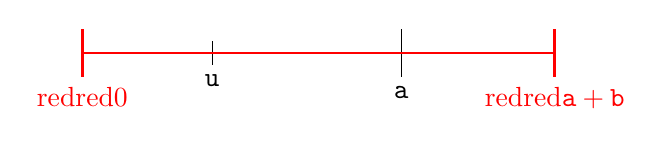
\begin{tikzpicture}[scale = 1.5, domain = -.5 : 6.5]
            \tikzstyle{mybox} = [rounded corners = 0pt] %
            \tikzstyle{fancytitle} = [rounded corners = 0pt] %
            \def\debSeg{0}; % la valeur de epsilon
            \def\finSeg{4}; % la valeur (exacte) de epsilon
            \def\color{red}; % la couleur choisie
            \def\r{1.1}; %
            \def\seuil{2.7};
            
            \draw[-] (\r,.1) -- (\r,-.1) node[below] {\tt u}; %
            \draw[-] (\seuil,.2) -- (\seuil,-.2) node[below]
            {$\mathtt{a}$}; %
            
            \draw[-, very thick, color = \color] (\debSeg,.2) --
            (\debSeg,-.2) node[below] {$0$}; %
            \draw[-, very thick, color = \color] (\finSeg,.2) --
            (\finSeg,-.2) node[below] {$\mathtt{a+b}$}; %
            
            \draw[-] (\debSeg, 0) -- (\finSeg, 0) ; % segment [0,1]
            
            \draw[-, color=\color, thick] ({\debSeg}, 0) --
            ({\finSeg}, 0); %
          \end{tikzpicture}
        \end{center}
        Le réel {\tt u} appartient à l'intervalle $[0, \mathtt{a}[$
        avec probabilité :
        \[
        \Prob\left(\Ev{U \in [0, \mathtt{a}[ \ } \right) =
        \Prob\left(\Ev{U < \mathtt{a}} \right) =
        \dfrac{\mathtt{a}}{\mathtt{a+b}} = \Prob(\Ev{X_1 = 1})
        \]
        Le réel {\tt u} appartient à l'intervalle $[\mathtt{a},
        \mathtt{a+b}[$ avec probabilité :
        \[
        \Prob\left(\Ev{ U \in [\mathtt{a}, \mathtt{a+b}[ \ } \right) =
        \Prob\left(\Ev{ U \geq \mathtt{a}} \right) =
        \dfrac{\mathtt{b}}{\mathtt{a+b}} = \Prob(\Ev{X_1 = 0})
        \]
        C'est ce que réalise le programme en ligne \ligne{6} :
        \begin{scilabC}{4}
          & \qquad \tcIf{if} (u < \tcVar{a}) \tcIf{then} \nl %
          & \qquad \qquad \tcVar{x}(1,1) = 1 \nl %
        \end{scilabC}
        Dans le cas où la condition n'est pas réalisée (ce qui se
        produit avec probabilité $\frac{\mathtt{b}}{\mathtt{a+b}}$) le
        premier coefficient de la matrice {\tt x} n'est pas mis à
        jour.

      \item on simule ensuite la \var $X_2$.\\
        Pour ce faire, on regarde la valeur {\tt x(1,1)} simulée pour
        $X_1$ :
        \begin{noliste}{-}
        \item Si {\tt x(1,1)} vaut $1$ alors $X_2$ doit prendre la
          valeur $1$ avec probabilité $\dfrac{\mathtt{a} +
            1}{\mathtt{a+b} + 1}$.\\
          {\it (d'après la question \itbf{8.c)} : $\Prob_{\Ev{X_1 =
                1}}\big( \Ev{X_2 = 1} \big) \ = \
            \dfrac{a+1}{a+b+1}$)}\\
        Pour affecter à {\tt x(1,2)} la bonne valeur, on procède comme
        pour {\tt x(1,1)}.\\
        Le schéma est le suivant :
        \begin{center}
          %% French babel fout la merde : ne pas oublier shorthandoff
          \shorthandoff{;} %
          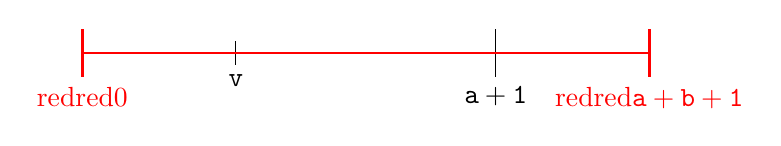
\begin{tikzpicture}[scale = 1.5, domain = -.5 : 6.5]
            \tikzstyle{mybox} = [rounded corners = 0pt] %
            \tikzstyle{fancytitle} = [rounded corners = 0pt] %
            \def\debSeg{0}; % la valeur de epsilon
            \def\finSeg{4.8}; % la valeur (exacte) de epsilon
            \def\color{red}; % la couleur choisie
            \def\r{1.3}; %
            \def\seuil{3.5};
            
            \draw[-] (\r,.1) -- (\r,-.1) node[below] {\tt v}; %
            \draw[-] (\seuil,.2) -- (\seuil,-.2) node[below]
            {$\mathtt{a+1}$}; %
            
            \draw[-, very thick, color = \color] (\debSeg,.2) --
            (\debSeg,-.2) node[below] {$0$}; %
            \draw[-, very thick, color = \color] (\finSeg,.2) --
            (\finSeg,-.2) node[below] {$\mathtt{a+b+1}$}; %
            
            \draw[-] (\debSeg, 0) -- (\finSeg, 0) ; % segment [0,1]
            
            \draw[-, color=\color, thick] ({\debSeg}, 0) --
            ({\finSeg}, 0); %
          \end{tikzpicture}
        \end{center}          
        On complète donc comme suit la ligne \ligne{7} :
        \begin{scilabC}{6}
          & \qquad \qquad \tcIf{if} (v < a + 1) \tcIf{then} \nl %
          & \qquad \qquad \qquad \tcVar{x}(1,2) = 1 \nl %
        \end{scilabC}

        \item Si {\tt x(1,1)} vaut $0$ alors $X_2$ doit prendre la
          valeur $1$ avec probabilité :
          \[
          \begin{array}{rcl@{\quad}>{\it}R{5cm}}
            \Prob_{\Ev{X_1 = 0}}\big( \Ev{X_2 = 1} \big) & = &
            \dfrac{\Prob\big( \Ev{X_1 = 0} \cap \Ev{X_2 =
                1}\big)}{\Prob\big( \Ev{X_1 = 0} \big)} 
            \\[.6cm]
            & = &
            \dfrac{\frac{ab}{(a+b+1) (a+b)}}{\frac{b}{a+b}} \ = \
            \dfrac{ab}{(a+b+1) \bcancel{(a+b)}} \
            \dfrac{\bcancel{a+b}}{b} \ = \ \dfrac{a}{a+b+1}
          \end{array}
          \]
          Pour affecter à {\tt x(1,2)} la bonne valeur, on procède
          comme précédent.\\
          Le schéma est le suivant :
        \begin{center}
          %% French babel fout la merde : ne pas oublier shorthandoff
          \shorthandoff{;} %
          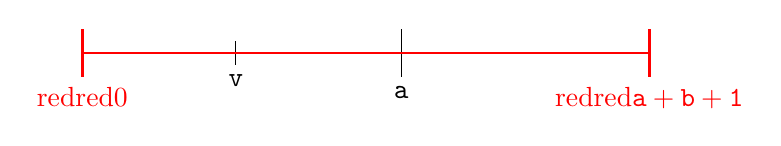
\begin{tikzpicture}[scale = 1.5, domain = -.5 : 6.5]
            \tikzstyle{mybox} = [rounded corners = 0pt] %
            \tikzstyle{fancytitle} = [rounded corners = 0pt] %
            \def\debSeg{0}; % la valeur de epsilon
            \def\finSeg{4.8}; % la valeur (exacte) de epsilon
            \def\color{red}; % la couleur choisie
            \def\r{1.3}; %
            \def\seuil{2.7};
            
            \draw[-] (\r,.1) -- (\r,-.1) node[below] {\tt v}; %
            \draw[-] (\seuil,.2) -- (\seuil,-.2) node[below]
            {$\mathtt{a}$}; %
            
            \draw[-, very thick, color = \color] (\debSeg,.2) --
            (\debSeg,-.2) node[below] {$0$}; %
            \draw[-, very thick, color = \color] (\finSeg,.2) --
            (\finSeg,-.2) node[below] {$\mathtt{a+b+1}$}; %
            
            \draw[-] (\debSeg, 0) -- (\finSeg, 0) ; % segment [0,1]
            
            \draw[-, color=\color, thick] ({\debSeg}, 0) --
            ({\finSeg}, 0); %
          \end{tikzpicture}
        \end{center}          
        On complète donc comme suit la ligne \ligne{11} :
        \begin{scilabC}{6}
          & \qquad \qquad \tcIf{if} (v < a) \tcIf{then} \nl %
          & \qquad \qquad \qquad \tcVar{x}(1,2) = 1 \nl %
        \end{scilabC}~\\[-1cm]
      \end{noliste}
    \end{noliste}
  \end{noliste}
  \begin{remark}%~
    Rappelons qu'on détaille la réponse à cette question afin de
    permettre une bonne compréhension des mécanismes en
    jeu. Cependant, compléter correctement le programme \Scilab{}
    démontre la bonne compréhension de la simulation demandée et
    permet certainement d'obtenir tous les points alloués à cette
    question.
  \end{remark}~\\[-1.2cm]
\end{proof}
\end{liste}


\newpage

  
\begin{noliste}{1.}
  \setcounter{enumi}{9} %
  \setlength{\itemsep}{4mm}
\item
  \begin{noliste}{a)}
    \setlength{\itemsep}{2mm}
  \item Calculer le coefficient de corrélation linéaire de $X_1$ et
    $X_2$.
      
    \begin{proof}~%
      \begin{noliste}{$\sbullet$}
      \item Les \var $Y_1$ et $Y_2$ sont finies donc elles admettent
        chacune un moment d'ordre $2$.\\
        Ainsi, $Y_1$ et $Y_2$ admettent un coefficient de corrélation
        linéaire donné par :
        \[
        \rho(X_1, X_2) \ = \ \dfrac{\Cov(X_1, X_2)}{\sqrt{\V(X_1)
            \V(X_2)}} \ = \ \dfrac{\E(X_1X_2) - \E(X_1)
          \E(X_2)}{\sqrt{\V(X_1) \V(X_2)}}
        \]
        Or $X_1$ et $X_2$ suivent la même loi $\Bern{\dfrac{a}{a+b}}$.
        Ainsi :
        \[
        \begin{array}{rcl}
          \E(X_1) & = & \dfrac{a}{a+b} \ = \ \E(X_2)
          \\[.6cm]
          \V(X_1) & = & \dfrac{a}{a+b} \left( 1 - \dfrac{a}{a+b}
          \right) \ = \ \dfrac{a}{a+b} \ \dfrac{b}{a+b} \ = \ \V(X_2)
        \end{array}
        \]

      \item L'espérance $\E(X_1X_2)$ est définie par :
        \[
        \begin{array}{rcl@{\quad}>{\it}R{5cm}}
          \E(X_1 X_2) & = & \Sum{i = 0}{1} \left( \Sum{j = 0}{1} i \ j \
            \Prob\big( \Ev{X_1 = i} \cap \Ev{X_2 = j}\big) \right)
          \\[.6cm]
          & = & \Prob\big( \Ev{X_1 = 1} \cap \Ev{X_2 = 1} \big)
          \\[.2cm]
          & = & \dfrac{(a+1) \ a}{(a+b+1) (a+b)} 
        \end{array}
        \]
        Ainsi :
        \[
        \begin{array}{rcl@{\quad}>{\it}R{5cm}}
          \E(X_1 X_2) - \E(X_1) \E(X_2) & = & \dfrac{(a+1) \ a}{(a+b+1)
            (a+b)} - \dfrac{a}{a+b} \ \dfrac{a}{a+b} 
          \\[.6cm]
          & = & \dfrac{a}{a+b} \ \left( \dfrac{a+1}{a+b+1} -
            \dfrac{a}{a+b} \right) 
          \\[.6cm]
          & = & \dfrac{a}{a+b} \ \left( \dfrac{(a+1)(a+b) -
              a(a+b+1)}{(a+b+1)(a+b)} \right)
          \\[.6cm]
          & = & \dfrac{a}{a+b} \ \left( \dfrac{(a^2+ab+a+b) -
              (a^2+ab+a)}{(a+b+1)(a+b)} \ \right)
          \\[.6cm]
          & = & \dfrac{a}{a+b} \ \dfrac{b}{(a+b+1)(a+b)} \ = \
          \dfrac{ab}{(a+b+1)(a+b)^2} 
        \end{array}
        \]
        
      \item On peut alors finir le calcul :
        \[
        \begin{array}{rcl@{\quad}>{\it}R{5cm}}
          \rho(X_1, X_2) & = & \dfrac{1}{\sqrt{\V(X_1) \V(X_2)}} \ \big(
          \E(X_1 X_2) - \E(X_1) \E(X_2) \big)
          \\[.6cm]
          & = & \dfrac{(a+b)^2}{\bcancel{ab}} \
          \dfrac{\bcancel{ab}}{(a+b+1)(a+b)^2} \ = \ \dfrac{1}{a + b + 1} 
        \end{array}
        \]
      \end{noliste}
      \conc{$\rho(X_1, X_2) \ = \ \dfrac{1}{a + b + 1}$}~\\[-1cm]
    \end{proof}


    \newpage


  \item Soit $(p,r)$ un couple de réels vérifiant $0 < p < 1$ et $0 <
    r < 1$.\\
    Expliquer comment utiliser la fonction {\tt randbetabin} pour
    simuler deux variables aléatoires suivant une même loi de
    Bernoulli de paramètre $p$ et dont le coefficient de corrélation
    linéaire est égal à $r$.

    \begin{proof}~%
      \begin{noliste}{$\sbullet$}
      \item La fonction {\tt randbetabin} prend pour paramètres les
        variables {\tt a} et {\tt b} et renvoie la simulation du
        couple $(X_1, X_2)$, où $X_1$ et $X_2$ suivent toutes les deux
        la même loi de Bernoulli $\Bern{\dfrac{\mathtt{a}}{\mathtt{a +
              b}}}$.

      \item Ainsi, si on souhaite utiliser la fonction {\tt
          randbetabin} pour simuler deux variables aléatoires suivant
        une même loi de Bernoulli de paramètre $p$ et dont le
        coefficient de corrélation linéaire est égal à $r$, il suffit
        de trouver {\tt a} et {\tt b} solutions du système $(S)$
        suivant :
        \[
        (S) \ 
        \left\{
          \begin{array}{rcl}
            p & = & \dfrac{a}{a+b}
            \\[.4cm]
            r & = & \dfrac{1}{a+b+1}
          \end{array}
        \right.
        \]

      \item Résolvons ce système :
        \[
        \begin{array}{rcl@{\quad}>{\it}R{4.8cm}}
          (S) & \Longleftrightarrow &         
          \left\{
            \begin{array}{rcrcl}
              (p-1) \ a & + & p \ b & = & 0
              \\[.2cm]
              r \ a & + & r \ b & = & 1 - r
            \end{array}
          \right.
          & (en multipliant $L_1$ par $a+b$ et $L_2$ par $a+b+1$ et en
          réordonnant) 
          \nl
          \nl%[.8cm]
          & 
          \begin{arrayEq}
            L_2 \leftarrow (p-1) \ L_2 - r \ L_1 
          \end{arrayEq}
          &         
          \left\{
            \begin{array}{rcrcl}
              (p-1) \ a & + & p \ b & = & 0
              \\[.2cm]
              & - & r \ b & = & (p - 1)(1 - r)
            \end{array}
          \right.
          & (avec $p-1 \neq 0$ car $p \neq 1$)
          \nl
          \nl
          &
          \begin{arrayEq}
            L_1 \leftarrow r \ L_1 + p \ L_2 
          \end{arrayEq}
          &         
          \left\{
            \begin{array}{rcrcl}
              r (p-1) \ a & & & = & p(p - 1)(1 - r)
              \\[.2cm]
              & - & r \ b & = & (p - 1)(1 - r)
            \end{array}
          \right.
          &
          (avec $r \neq 0$)
          \nl
          \nl
          &
          \begin{arrayEq}
            L_1 \leftarrow \frac{1}{r(p-1)} \ L_1 \\
            L_2 \leftarrow -\frac{1}{r} \ L_2
          \end{arrayEq}
          &         
          \left\{
            \begin{array}{rcrcl}
              a & & & = & p \ \dfrac{1 - r}{r}
              \\[.2cm]
              & & b & = & (1 - p) \ \dfrac{1 - r}{r}
            \end{array}
          \right.
          & (avec $r(p-1) \neq 0$)
        \end{array}
        \]
      \end{noliste}
      \concL{Pour {\tt p} et {\tt r} donnés, l'appel {\tt
          randbetabin(p\Sfois{}(1-r)/r, (1-p)\Sfois{}(1-r)/r)} permet
        d'obtenir la simulation de \var $X_1$ et $X_2$ qui vérifient
        les propriétés énoncées dans la question.}{15.4}~\\[-.8cm]
    \end{proof}

  \end{noliste}
\end{noliste}

